\documentclass[11pt,a4paper]{report}
\usepackage[utf8]{inputenc}
\usepackage[T1]{fontenc}
\usepackage{geometry}
\geometry{left=2.7cm,right=2.7cm,top=2.6cm,bottom=2.6cm}
\usepackage{lmodern,microtype,setspace}
\usepackage{graphicx,float,amsmath,amssymb,cite,listings,xcolor,booktabs,array,caption,subcaption,algorithm,algpseudocode,tikz,pgfplots,seqsplit}
% siunitx formats the measured statistics so that thousands separators are
% restored without truncating the fractional part the receipts record.
% `output-decimal-marker` and `group-digits=integer` are required: siunitx
% otherwise defaults to grouping every digit run and uses a French-style decimal
% mark, which rendered a timing value of 23960.5423 as `23,960.542,3`.
\usepackage[
  group-separator={,},
  group-minimum-digits=4,
  group-digits=integer,
  output-decimal-marker={.},
  round-mode=places,
  round-precision=4,
  round-pad=false
]{siunitx}
\usepackage[hidelinks]{hyperref}
\pgfplotsset{compat=1.18}
\usetikzlibrary{shapes,arrows,positioning,fit,backgrounds,matrix,calc}
\onehalfspacing
\setlength{\parindent}{1.5em}
\setlength{\parskip}{0.15em}
\setlength{\emergencystretch}{2em}
\hypersetup{pdftitle={Privacy Lens: Regulation-Driven Temporal Privacy Review},pdfauthor={Zhiheng Zhang}}
% Record pointers resolve to the pinned public artifact revision, so every
% location the thesis directs a reader to can be opened and checked directly.
\newcommand{\RepoURL}{https://github.com/zhiheng-zhang-Mera/privacy-lens-research-artifact}
\newcommand{\RepoCommit}{fe4b11bc5337d37a0e8b50856ab338001123d5c4}
\newcommand{\RepoTree}[1]{\href{\RepoURL/tree/\RepoCommit/#1}{\texttt{\seqsplit{#1}}}}
\newcommand{\RepoBlob}[1]{\href{\RepoURL/blob/\RepoCommit/#1}{\texttt{\seqsplit{#1}}}}
\newcommand{\RepoCommitLink}[2]{\href{\RepoURL/commit/#1}{\texttt{#2}}}
\title{Privacy Lens: Evidence-Bounded Android Privacy Review with Regulation-Driven Temporal Combination Notices}
\newif\ifsubmissionedition
\ifdefined\PrivacyLensSubmissionEdition
  \submissioneditiontrue
\else
  \submissioneditionfalse
\fi
\ifsubmissionedition
  \IfFileExists{private-submission-metadata.tex}{\input{private-submission-metadata}}{%
    \newcommand{\PrivacyLensStudentID}{NOT PROVIDED}%
    \newcommand{\PrivacyLensSupervisor}{NOT PROVIDED}%
  }
  \author{Zhiheng Zhang \\ Student ID: \PrivacyLensStudentID \\ Supervisor: \PrivacyLensSupervisor}
\else
  \author{Zhiheng Zhang}
\fi
\date{September 2026}
% Generated by scripts/verify-thesis-evidence.js --write. Do not edit manually.
\newcommand{\PrivacyLensVersion}{1.15.0}
\newcommand{\FDroidCensusN}{495}
\newcommand{\FDroidSensitiveN}{125}
\newcommand{\FDroidSensitiveNetworkN}{74}
\newcommand{\FDroidSensitiveBackgroundN}{74}
\newcommand{\FDroidMultiProcessN}{54}
\newcommand{\DevicePackagesN}{233}
\newcommand{\CompletedWorkflowsN}{203}
\newcommand{\FailedDeviceWorkflowsN}{30}
\newcommand{\PssObservedN}{98}
\newcommand{\TimingObservedN}{101}
\newcommand{\DevicePssMedianKb}{53603.5}
\newcommand{\DevicePssQOneKb}{47884}
\newcommand{\DevicePssQThreeKb}{64831.25}
\newcommand{\DeviceTimingMedianMs}{23960.5423}
\newcommand{\DeviceTimingQOneMs}{21494.4533}
\newcommand{\DeviceTimingQThreeMs}{25115.4851}
\newcommand{\FlowDroidReceiptsN}{1}
\newcommand{\FlowDroidXmlArtifactsN}{0}
\newcommand{\StressCorpusN}{40,000}
\newcommand{\StressRestartN}{10,000}
\newcommand{\StressMalformedN}{20,000}
\newcommand{\StressAssertionsN}{112,236}
\newcommand{\StressRuleMatchesN}{22,246}

\begin{document}
\maketitle
\begin{abstract}
\small\singlespacing
Privacy Lens is a local-first Android research prototype that transforms heterogeneous, bounded privacy evidence into review prompts without treating a technical signal as proof of purpose, necessity, lawful basis, compliance, or intent. Its fail-closed pipeline preserves provenance, temporal scope, regulation-pack identity, missing context, and unavailable outputs through admission, temporal combination, typed policy interpretation, persistence, and presentation.

The thesis reports three contributions. The first is a set of cross-layer evidence-bounded contracts: source, missing context, pack identity, and permitted output are carried as one inspectable interface and state contract from admission to presentation, and the permitted output domain excludes legal verdicts. The second is bounded temporal combination and state-continuity semantics: replay, overlap, source and pack isolation, order, and recovery receive explicit conditions, and the losses that remain are stated rather than hidden. The third is a layered, diagnostic evaluation that reports unlike evidence objects with separate denominators, retains failures and missing values, names the oracle tier of each suite, and draws a transferable finding from what the existing records do and do not show.

The strongest external engineering evidence comprises a hash-pinned open-source census of \FDroidCensusN{} APKs, bounded physical-device workflows for \DevicePackagesN{} package identities with \CompletedWorkflowsN{} completed and \FailedDeviceWorkflowsN{} retained failures, and a one-device interface record for release \PrivacyLensVersion{}. Missing static-analysis artifacts remain missing evidence, corpus-derived counts are not converted into legal labels, and counts drawn from different evidence objects are never summed. These results support reproducible engineering claims only: independent legal mapping review, participant comprehension, multi-OEM replication, population accuracy, production signing, and store acceptance remain unestablished.
\end{abstract}
\newpage
\tableofcontents
\newpage
\chapter{Introduction}

This chapter defines the problem that Privacy Lens is designed to solve and the claims that the thesis is prepared to defend. The central concern is not whether Android exposes a permission fact, but whether that fact can be transformed into a useful review prompt without acquiring legal meaning that the evidence does not contain. The chapter therefore moves from the mobile privacy context to the evidence-to-decision problem, the research questions, and the contribution boundary.

\section{Problem Statement: The Evidence-to-Decision Gap}

Mobile applications ask users to make privacy decisions while the evidence needed to evaluate those decisions remains fragmented. A permission declaration states capability, not necessarily use; a runtime observation can indicate activity, but not purpose, lawful basis, necessity, or proportionality. The Regulation requires legal and organisational analysis in addition to technical safeguards, including the principles in Article 5 and data protection by design and by default in Article 25 \cite{gdpr2016,edpbArticle25}.

Privacy Lens addresses a narrower engineering problem: how can an ordinary Android application present available permission-audit evidence without transforming incomplete telemetry into a false legal conclusion? The application collects no remote evidence, has no account or advertising layer, and stores findings locally. It exposes whether a finding came from device-visible observations or a synthetic demonstration, displays missing-evidence limitations, and prepares questions for human review.

The work began as a GDPR-oriented prototype. The evaluated release retains the GDPR as its legal objective but removes jurisdiction-specific interpretation from the core decision mechanism. Legal mappings are loaded through replaceable regulation packs. This separation makes regional extension possible while preventing the interface, repository, and Android bridge from silently inheriting one jurisdiction's terminology.

The position this thesis argues for can be stated in one sentence: technical observations should retain their provenance, temporal scope, rule identity, and missing context as they are admitted, combined over time, interpreted against a mounted rule pack, persisted, and presented, and bounded evidence should be prevented from becoming an unsupported legal conclusion along those modelled paths. This is the working centre of the argument, not a proved whole-system theorem. Each clause is tightened later against the implemented behaviour and the witnesses that actually exist, and the thesis states where a modelled path is not covered.

\section{Why Mobile Permission Evidence Matters}

Mobile privacy is difficult to reason about because a handheld device combines intimate data, continuous availability, and many independent software actors. A user may encounter an application as a single icon, yet that application can depend on operating-system services, embedded libraries, cloud endpoints, analytics components, advertising identifiers, and background tasks. The apparent simplicity of a permission prompt therefore hides a larger processing system. The prompt may describe access to a sensor or data category, but it does not normally explain every purpose, recipient, retention period, inference, or downstream combination. Contextual integrity theory is useful here because it treats privacy as the appropriateness of information flows within a social context rather than as secrecy alone \cite{nissenbaum2011}. A technically permitted flow can still be surprising or inappropriate when its purpose, recipient, or persistence differs from the context understood by the user.

The mismatch matters across application domains because camera, microphone, location, contacts, and activity signals can reveal sensitive behaviour even when an operating-system permission is technically valid. Privacy Lens therefore does not infer purpose or legality from a permission name. It preserves the observed signal, its source, its time window, and the questions that remain unanswered. This domain-neutral position keeps the architecture applicable to different application categories without claiming knowledge that the evidence contract does not contain.

Android's permission model provides necessary protection, but permission state and processing purpose are different constructs. A granted permission indicates that an application may invoke a protected capability under specified platform conditions. It does not state whether the capability was invoked, why an invocation occurred, whether derived data were retained, or whether the processing satisfied a legal obligation. Conversely, a denied or absent permission does not prove the absence of all related data because an application may receive information through another service, user input, previously collected records, or a less sensitive signal from which attributes can be inferred. The prototype therefore treats permission observations as one evidence family within a broader review, not as a complete representation of processing.

\section{From Technical Signal to Review Finding}

The central research problem can be described as an evidence-to-decision gap. At one end of the gap are platform facts: a package identifier, permission category, access count, observation window, acquisition source, and timestamp. At the other end are questions that matter to a person or regulator: Was processing expected? Was it necessary for the stated purpose? Was a valid lawful basis available? Were special-category conditions satisfied? Were recipients and retention disclosed? Was the data subject able to exercise meaningful control? No deterministic transformation can recover answers that were never present in the input.

Two common design errors follow from ignoring this gap. The first is semantic inflation, in which a technical event is labelled as a legal violation. This gives a small signal the authority of a much broader assessment. The second is evidential silence, in which an empty or unavailable audit is displayed as a reassuring green state. On stock Android, ordinary applications often lack authority to inspect unrestricted cross-application history. Treating an empty result as absence of activity would therefore reward the system precisely when its visibility is weakest.

Privacy Lens introduces an intermediate output: a review finding. A finding can say that the available count crossed a research threshold, that evidence is unavailable, or that no technical concern was identified within the observed window. It can also state which contextual facts are missing. This format preserves utility without claiming certainty. The distinction is comparable to the difference between a screening instrument and a diagnosis: screening can identify cases that deserve attention, but its result must be interpreted in context and by an appropriately qualified actor.

The design also recognises that explanation is not an optional layer added after computation. Explanation begins with data modelling. If the repository stores only a severity colour and a message, the interface cannot later reconstruct the source, rule version, temporal scope, or missing context. The system consequently defines provenance fields as part of the decision object. The interface is a view of that object rather than a separate narrative that can drift away from it.

\section{Consent, Attention, and Interface Burden}

Privacy interfaces operate under severe attention constraints. McDonald and Cranor quantified the impractical time cost of reading the privacy policies encountered by an ordinary user \cite{mcdonald2008}. Obar and Oeldorf-Hirsch demonstrated how readily people accept online terms without substantive engagement \cite{obar2020}. These findings should not be interpreted as evidence that users are careless. They show that notice-and-choice systems frequently demand more time and legal comprehension than a routine interaction can support.

A warning application can reproduce this failure if it presents a wall of legal text, asks the user to interpret raw telemetry, or interrupts every time a count changes. More information is not automatically more usable transparency. Information must be staged according to the decision a user can reasonably make. Privacy Lens therefore begins with three questions: what requires attention, what evidence is missing, and what can be done next. Rule references and technical details remain available, but they follow the status and action rather than preceding them.

This approach also affects notification strategy. Repeated alerts for an unchanged state can teach users to ignore the product. A review system should distinguish new evidence, a material escalation, and a stable finding. Although the present candidate does not claim a longitudinal notification study, its repository retains enough state to support transition-based notification in future work. The architectural principle is that attention is a limited resource and should be consumed only when evidence meaningfully changes.

\section{Accountability Rather Than Automated Adjudication}

The GDPR's accountability principle requires a controller not only to comply with the Regulation but also to be able to demonstrate compliance \cite{gdpr2016}. A consumer-facing application cannot fulfil the controller's entire accountability obligation, because it does not possess the controller's records of processing, contracts, purposes, retention decisions, risk assessments, or organisational measures. It can nevertheless support accountability by making a narrow technical observation reproducible and by showing which questions remain unanswered.

This positioning changes the desired failure mode. A conventional classifier may optimise for a single label and treat rejected input as an implementation inconvenience. An accountability tool should prefer an explicit hold or evidence gap to a falsely reassuring result. Unsafe types, unrecognised sources, impossible windows, and missing context therefore fail closed. The system does not invent a value to keep the pipeline moving. This behaviour is especially important at a native bridge, where JavaScript assumptions can be violated by malformed, stale, or unexpected platform data.

Accountability also requires version knowledge. A finding that says only GDPR is not reproducible if rules or interpretations later change. Privacy Lens records a pack identifier and version, an official source, and a particular rule reference. Historical findings are not silently reinterpreted when the active pack changes. This creates a minimal audit trail: a reviewer can identify which data were available, which pack was applied, and why a particular message appeared.

\section{Regional Extensibility as a Governance Problem}

The request for regional switching creates both an architectural opportunity and a governance risk. It is straightforward to define a common software interface for multiple packs. It is much harder to ensure that each pack represents its jurisdiction accurately. Legal systems differ in scope, terminology, actors, exemptions, enforcement, and the relationship between national and sectoral rules. A design that assumes every jurisdiction can be translated into GDPR article equivalents would merely hide legal coupling behind a new file format.

The evaluated prototype therefore separates software extensibility from legal validity. The registry proves that the application can discover, select, persist, and apply different pack objects. It does not certify the content of every possible pack. The EU GDPR pack is the evaluated legal objective. The Research Baseline pack is deliberately non-legal and demonstrates the mechanism without suggesting that another jurisdiction has been reviewed. A future regional pack must identify its authority, effective date, scope, official source, reviewer, localisation status, fixtures, migration policy, and limitations.

This distinction is central to the thesis contribution. Decoupling is valuable not because it makes law interchangeable, but because it makes jurisdiction-dependent assumptions visible and reviewable. When a legal mapping is isolated, it can be versioned, challenged, replaced, and tested without changing the Android bridge or product shell. The architecture therefore supports expansion while making the cost of responsible expansion explicit.

\section{Research Method}

The work follows an iterative design-and-evaluation method. First, legal and platform constraints are translated into claim boundaries. Second, these boundaries become data and interface requirements. Third, the requirements are implemented across TypeScript, React Native, Kotlin, storage, and Android build configuration. Fourth, each layer is evaluated with evidence appropriate to that layer. Finally, contradictions between intended claims and observed behaviour are used to revise both code and thesis.

The method combines constructive and empirical elements. The constructive element is the artefact: the evidence contract, temporal ledger, rule-pack compiler, typed policy graph, repository, FlowDroid adapter, Android bridge, and interface. The empirical element consists of the deterministic and adversarial suites, a hash-pinned \FDroidCensusN{}-APK static census, \DevicePackagesN{} bounded package workflows on one device, static-analysis receipts, and bounded device records; Chapter 5 states the unit and denominator of each. The method does not include a controlled participant experiment or completed independent legal mapping review; those omissions are recorded as limitations rather than replaced with speculative conclusions.

One methodological rule governs the rest: evidence is not pooled across incompatible layers, because a thousand logical cases are not a thousand device trials, a successful installation does not validate every scheduled task, a rendered warning does not prove comprehension, and a rule reference does not prove infringement.

\section{Research Questions}

The thesis answers four questions that connect evidence admission, communication, extensibility, and evaluation.

\textbf{RQ1: How can heterogeneous Android privacy evidence be admitted and transformed into deterministic review findings while malformed, replayed, overlapping, or provenance-incompatible evidence fails closed?} This question concerns the runtime evidence contract, decision semantics, temporal isolation, replay behaviour, and restart state. It is evaluated through exact-boundary, adversarial, permutation, stateful, and fixed-seed stress tests.

\textbf{RQ2: How can provenance, temporal scope, rule identity, and missing context be represented and presented without encoding a legal verdict into the system state?} This question concerns finding construction, typed policy output, dashboard projection, status language, source disclosure, and the distinction between synthetic evidence and device-visible observations. It is evaluated at the representation and implementation levels through policy fixtures, presentation contracts, and recorded workflows; participant comprehension remains future empirical work.

\textbf{RQ3: How can jurisdiction-dependent review logic be isolated behind versioned regulation-pack and formal-policy boundaries while preserving traceability and historical identity?} This question concerns registry admission, pack compilation, policy output restrictions, immutable metadata, historical identity, and visible caveats. It is evaluated by applying admitted evidence under registered packs and checking cross-pack isolation and retained finding identity.

\textbf{RQ4: What claims are supported when the framework is evaluated across deterministic fixtures, adversarial properties, real application artifacts, static-analysis outputs, and bounded physical-device execution?} This question concerns evidence strength and external validity. It is answered through a claim-to-evidence matrix that keeps semantic, interoperability, external-engineering, human, legal, and deployment claims separate.

Table~\ref{tab:rq-evidence-map} makes the evidential contract for each question explicit. A method can answer only the question assigned to it; evidence is not pooled across rows to manufacture a stronger result.

\begin{table}[H]
\centering
\caption{Research-question to evidence map}
\label{tab:rq-evidence-map}
\scriptsize
\setlength{\tabcolsep}{3pt}
\begin{tabular}{>{\raggedright\arraybackslash}p{0.055\textwidth}>{\raggedright\arraybackslash}p{0.20\textwidth}>{\raggedright\arraybackslash}p{0.18\textwidth}>{\raggedright\arraybackslash}p{0.12\textwidth}>{\raggedright\arraybackslash}p{0.16\textwidth}>{\raggedright\arraybackslash}p{0.18\textwidth}}
\toprule
RQ & Method & Dataset or evidence & Metric or decision & Result location & Principal limitation \\
\midrule
RQ1 & Constructive implementation plus deterministic, adversarial, restart, replay, and mutation tests & Typed fixtures, 1,000 seeded cases, 720 permutations, nine curated mutants & Contract pass/fail, confusion cells, mutant detection & Chapters 3--5; safety-property catalogue & Oracle and implementation remain partly correlated; no field ground truth \\
RQ2 & Typed policy and presentation contracts plus bounded device walkthrough & Policy graphs, source checks, UI hierarchy, screenshots, decision-pause flow & Reachability of prohibited verdicts; presence of source, caveat, and missing context & Chapters 4--5; claim-evidence matrix & No participant comprehension or assistive-technology study \\
RQ3 & Pack admission, compiler, cross-pack isolation, historical binding, and mapping-review preparation & EU GDPR and non-legal Research Baseline packs; 13-item review packet & Pack validation, switching, isolation, retained identity & Chapters 3--5; mapping packet & Independent legal mapping review is \texttt{NOT\_RUN} \\
RQ4 & Triangulation across logical, corpus, static-analysis, package, and device layers & Hash-pinned F-Droid census, device receipts, FlowDroid receipt, final release package & Layer-specific denominators, failures, missing outputs, and package facts & Chapter 5; evidence manifest & No population, commercial-store, cross-device, legal, or human validity \\
\bottomrule
\end{tabular}
\end{table}

\section{Research Objectives and Contributions}

The research has four operational objectives. It must make each decision reproducible, communicate uncertainty without neutralising usefulness, isolate regional interpretation from generic product infrastructure, and produce an Android artefact that can be evaluated beyond source code. These objectives are realised through permission, source, time-window, pack, rationale, and missing-context fields; three non-verdict status classes; a registry of immutable pack definitions; and release APK and Android App Bundle outputs targeting SDK 36.

The thesis reports three contributions. The Android application, its interface, local storage, packaging, and the reproducibility toolchain are treated as implementation carriers or supporting evidence rather than as separate claims of novelty, unless they answer an independent research question with evidence of their own. This consolidation matters because a list of five or six co-equal contributions invites the reader to measure the project by the size of its component inventory instead of by the strength of its argument.

\begin{table}[H]
\centering
\caption{Contributions, principal evidence, and claim boundaries}
\label{tab:contribution-map}
\scriptsize
\setlength{\tabcolsep}{3pt}
\begin{tabular}{>{\raggedright\arraybackslash}p{0.045\textwidth}>{\raggedright\arraybackslash}p{0.16\textwidth}>{\raggedright\arraybackslash}p{0.26\textwidth}>{\raggedright\arraybackslash}p{0.235\textwidth}>{\raggedright\arraybackslash}p{0.20\textwidth}}
\toprule
ID & Contribution & Claim & Principal evidence & Boundary \\
\midrule
C1 & Cross-layer evidence-bounded contracts & Source, missing context, pack identity, and permitted output are carried as one inspectable interface and state contract from admission through presentation & Admission and type model; pack registry; finding and presentation contracts; traceability, package, and UI-hierarchy checks & Does not authenticate the input producer, create unavailable acquisition authority, or establish that a rendered caveat is understood \\
C2 & Bounded temporal combination and state continuity & Replay, overlap, source and pack isolation, order, and recovery receive explicit conditions and conservative treatment & Exact-boundary cases; 720 permutations; replay, overlap, restart, malformed-input, and stress records; pack switching & Cannot recover event information that was never recorded, and does not extend partial ledger recovery to every state object \\
C3 & Layered, diagnostic evaluation & Distinct evidence objects are reported with distinct denominators and conclusions, and existing mutation, failure, missingness, and missing-output records are analysed for what they do and do not show & Nine-of-nine registered mutant detections; corpus and device receipts; missing measurements; the no-XML static-analysis record & Not an external accuracy estimate, a causal study, evidence of user benefit, or independent legal validity \\
\bottomrule
\end{tabular}
\end{table}

Each contribution is only as strong as the analysis behind it, and the boundary of each is stated rather than implied. C1 does not claim that routine type checking, modular packing, or de-duplication are novel algorithms, and C2 does not claim novelty for replay suppression or bounded storage in general. C3 carries its weight by making the evidence separable: because each object keeps its own denominator, each suite names the tier of its oracle, and failures and missing values stay visible, a conformance result cannot be read as an accuracy claim and a curated mutant set cannot be read as a mutation score. The declared increment across the three is their combination under one evidence contract whose boundaries are stated in executable terms and tested wherever a witness exists.

The contribution is therefore not an automated GDPR judge. It is an accountability-support prototype that makes a bounded technical inference reconstructable and leaves legal conclusions to an appropriately authorised human reviewer. This positioning is narrower than the strongest claim a compliance application might advertise, but it is the strongest claim supported by the implemented evidence path.

\section{Scope and Claim Boundary}

The evaluated data path covers permission summary records available to the application or generated by its controlled simulator. Stock Android restricts ordinary applications from reading unrestricted activity belonging to other applications. Absence of an observation is consequently an evidence gap, not proof that an access did not occur. The current rule thresholds are research baselines; they are not statutory limits. The included EU GDPR pack is a traceable mapping aid, not legal advice.

Evaluation covers source compilation, deterministic and mutation-based property tests, typed-policy fixtures, release assembly, a \FDroidCensusN{}-APK static census, \DevicePackagesN{} bounded package workflows, FlowDroid-output adaptation, manifest inspection, installation, launch, interaction, and short-run observation on one OPPO PERM00 device. It does not establish multi-OEM compatibility, 24-hour scheduler reliability, battery performance, population accuracy, accessibility conformance, participant comprehension, independent legal validity, or application-store approval.

\section{Scope of the Evaluated System}

The evaluated system closes two deliberately narrow engineering gaps without expanding the prototype's claim. First, a minimal local temporal ledger makes an active, same-pack window survive process restart. Second, a Debug-only controlled device route exercises the normal native bridge with a fixture compiled from the mounted profile. Both additions preserve notification-only behaviour and label the controlled route as synthetic. They do not create real-world detection coverage, legal assurance, or cross-device reliability. The three contributions in Table~\ref{tab:contribution-map} should be read against this scope: C1 and C2 are claims about what the system preserves and refuses within these boundaries, and C3 is a claim about what the recorded evidence can and cannot establish.

\section{Thesis Structure}

Chapter 2 establishes the legal, Android, HCI, and software-architecture foundations. Chapter 3 derives requirements and the evidence-bounded architecture. Chapter 4 documents the implemented application and regulation-pack mechanism. Chapter 5 reports reproducible evaluation evidence. Chapter 6 analyses validity, usability, deployment, and legal limitations. Chapter 7 answers the research questions and defines the next validation programme. Two appendices support the argument without interrupting it: Appendix~\ref{app:ops} collects the operational, configuration and reproduction detail for the evaluated system, and Appendix~\ref{app:claims} records each core claim with its evidence type and its boundary.

In summary, the thesis begins from a semantic constraint: technical evidence can support review only when its acquisition scope and missing context remain visible. The next chapter positions this constraint within regulatory principles, Android platform semantics, human factors, and prior approaches to rule-based privacy support.

\chapter{Literature Review and Foundations}

This chapter examines four bodies of work that constrain the design: data-protection principles, Android observation mechanisms, human-centred warning design, and replaceable rule systems. The purpose is not to claim that Privacy Lens supersedes specialised legal, static-analysis, or enforcement tools. It is to identify the unresolved integration problem between a bounded technical observation and the conclusion a user is invited to draw from it.

\section{Review Protocol and Source Quality}

The chapter uses a structured scoping review rather than claiming a systematic review or meta-analysis. Sources were selected to answer four design questions: what a permission observation can establish, which legal facts it omits, how people interpret permission and warning interfaces, and how a replaceable decision mechanism can remain auditable. The final search date was 24 August 2026 and included official EU and Android material, peer-reviewed security and usable-privacy studies, standards, project-owned methodology, and foundational information-systems research. Seminal older work was retained when it defined a construct still used in the design, such as contextual integrity, cognitive load, trust calibration, usability, or design science. The search surfaces, seven representative query families, inclusion and exclusion rules, and the coding matrix are retained in \RepoBlob{docs/research/LITERATURE-REVIEW-PROTOCOL.md}. That protocol records no screening counts, no duplicate-screening step, and no PRISMA flow, so the coverage claimed for this chapter is the coverage of a documented scoping review with stated query families, not the coverage of an exhaustive or systematic search.

Source authority was ranked by the proposition being supported. Statutory meaning is grounded in the GDPR text and final EDPB guidance, not vendor summaries. Platform capability is grounded in Android documentation and bounded by installed-device evidence. Behavioural claims use original field or user studies and preserve their sample sizes and contexts. Engineering-method claims use original design-science publications \cite{hevner2004,peffers2007}. Standards and NIST privacy-engineering material are used as design guidance, not as proof of legal compliance \cite{nist8062,nistPrivacyFramework2020}. Commercial forecasts, uncited practitioner claims, and sources whose title or bibliographic record could not be verified were excluded from the thesis argument.

This protocol has limits. It does not report database-by-database recall, duplicate screening, or a PRISMA flow, and therefore must not be read as exhaustive coverage of mobile privacy research. Its purpose is narrower: make each source class and its evidential role explicit so that a reviewer can distinguish legal authority, platform specification, empirical user evidence, and design rationale.

The comparison matrix covers specialised but non-equivalent analytical objects. FlowDroid predicts potential static source-to-sink paths, while TaintDroid records selected flows under a modified runtime \cite{flowdroid2014,taintdroid2010}. Exodus matches embedded tracker signatures and expressly cautions that a match does not prove effective use \cite{exodusTrackerDetection}. PoliCheck relates observed flows to entity-sensitive policy statements, and contextual-integrity analysis exposes omitted or ambiguous transmission parameters \cite{policheck2020,shvartzshnaider2019}. Permission-dialog studies measure attention, comprehension, expectation, and decisions that source inspection cannot establish \cite{felt2012,bonne2017,cao2021}; field deployments add longitudinal evidence about permission changes and unusual access inside real usage contexts \cite{wijesekera2015,prange2024}; research on security warnings documents how repeated exposure can blunt the attention those interfaces depend on \cite{bravolillo2013attention,sunshine2009cryingwolf}. Android's Privacy Dashboard supplies an operating-system-owned history for supported permissions and windows, not purpose or legal meaning \cite{androidPrivacyDashboard}. These works motivate distinct evidence types; none is treated as a weaker implementation of one common classifier. Large-scale audits of health-related applications add population-level evidence that permissions and transmitted traffic can diverge from what a privacy policy states, while still leaving purpose and lawful basis unobserved \cite{tangari2021}.

Table~\ref{tab:related-work-comparison} records the comparison in the form used throughout this thesis: each approach is characterised by the evidence object it analyses, the output it is entitled to produce, and how it treats missing evidence. The table is not a ranking, and a blank or negative entry means only that the reviewed source does not report the property, not that the approach lacks it.

\begin{table}[H]
\centering
\scriptsize
\caption{Related-work comparison by evidence object and claim boundary}
\label{tab:related-work-comparison}
\begin{tabular}{>{\raggedright\arraybackslash}p{0.14\textwidth}>{\raggedright\arraybackslash}p{0.15\textwidth}>{\raggedright\arraybackslash}p{0.17\textwidth}>{\raggedright\arraybackslash}p{0.18\textwidth}>{\raggedright\arraybackslash}p{0.13\textwidth}}
\toprule
Approach & Evidence object & Supported output & Missing-evidence treatment & Relationship to Privacy Lens \\
\midrule
FlowDroid / TaintDroid & potential static paths / selected instrumented runtime flows & program-flow hypotheses / exercised-flow observations & unanalysed paths or executions are not negatives & upstream specialised evidence; no legal verdict \\
Exodus & embedded tracker signatures & tracker-presence indicators & a match does not prove effective use & complementary package evidence \\
PoliCheck / contextual integrity & observed flows plus policy or contextual parameters & consistency and contextual questions & omitted actors, purposes, or norms remain material & motivates explicit missing-context prompts \\
Permission-dialog studies & participant attention, comprehension, expectation, and choice & human-factor findings & untested populations and tasks limit transfer & required future validation of communication \\
Android Privacy Dashboard & OS-owned selected-permission history & bounded recent access history & unsupported permissions, windows, and context remain absent & possible authorised acquisition input \\
Privacy Lens & provenance-bound summaries plus versioned rule packs & technical review signals, evidence gaps, and questions & rejects unsafe input and shows unknown legal facts & integration and communication layer; not enforcement or certification \\
\bottomrule
\end{tabular}
\end{table}

\section{Regulatory Principles and Technical Signals}

The GDPR regulates processing rather than permission counts. Article 5 establishes principles including lawfulness, transparency, purpose limitation, data minimisation, accuracy, storage limitation, integrity, confidentiality, and accountability. Articles 6 and 9 concern lawful bases and special-category data; Article 25 requires data protection by design and by default \cite{gdpr2016}. EDPB guidance describes Article 25 as a continuing obligation implemented through appropriate technical and organisational measures \cite{edpbArticle25}. A technical observation may support an accountability inquiry, but cannot by itself demonstrate whether these legal conditions are satisfied.

This distinction determines the framework's vocabulary. A threshold exceedance is a \emph{review signal}. Missing purpose, lawful-basis, necessity, data-subject, controller, retention, and sharing evidence is shown explicitly. The UI never derives a finding labelled ``GDPR violation'' or ``compliant''. Regulation-pack references provide a reason to investigate and a link to an official source; they do not replace legal interpretation.

\subsection{From Legal Principle to Review Question}

Operationalisation is necessary in any regulatory technology, but it must preserve the semantic distance between a principle and a sensor. Article 5(1)(a) concerns lawfulness, fairness, and transparency. A permission count can contribute to transparency by revealing a pattern that was previously invisible, yet it cannot establish lawfulness or fairness. Article 5(1)(b) concerns purpose limitation. A count contains no purpose unless purpose is supplied as contextual evidence. Article 5(1)(c) concerns data minimisation. Frequency can be relevant to necessity, but a high frequency may be required for continuous navigation while a single collection may be excessive for an unrelated purpose. Article 5(2) concerns accountability. An audit record can support demonstration, but it is only one component of the records, decisions, safeguards, and governance required from a controller \cite{gdpr2016}.

Articles 6 and 9 further show why a permission signal cannot become a verdict. Article 6 provides several possible lawful bases; consent is not automatically the only basis and is subject to specific validity conditions \cite{edpbconsent2020}. Where consent is relied upon, a single notice is not the only model: consent can also be treated as a continuing relationship in which preferences are revisited over time, which is closer to what this framework asks of a reviewer than a one-off acceptance event \cite{kaye2015}. Article 9 establishes a prohibition and exceptions for special categories, but not every Android dangerous permission maps directly to special-category processing. Location, contacts, microphone, and camera data are context-dependent. Audio might contain health information, ordinary conversation, environmental noise, or no retained personal data. A technically observed invocation does not identify which of those states occurred.

The pack therefore maps a signal to a sequence of questions. For a location-related pattern, the reviewer may ask what purpose was declared, whether continuous precision was necessary, whether a less intrusive source was available, whether the application was in the foreground, whether location was retained or transmitted, and whether the user could reasonably anticipate the flow. For a microphone-related pattern, the reviewer may ask whether recording was user-initiated, how activation was signalled, whether raw audio left the device, and how long any derivative was retained. These questions are not answers; their value is that they prevent the visible count from crowding out legally decisive facts.

\subsection{Data Protection by Design and Interface Conduct}

Article 25 directs controllers to implement appropriate measures and privacy-protective defaults, taking account of state of the art, cost, context, and risk. EDPB guidance emphasises that this is a continuing obligation rather than a certification achieved once \cite{edpbArticle25}. For Privacy Lens, data protection by design affects both internal processing and the claims made to users. Local storage, disabled backup, no analytics, no advertising, no account, explicit deletion, and minimised permissions reduce the application's own data footprint. Fail-closed validation and immutable pack metadata reduce the risk that incomplete evidence becomes a misleading result.

Interface conduct is also relevant. A privacy tool could employ alarming colours, default users into sharing diagnostic data, hide evidence limitations, or imply that purchasing a service resolves risk. EDPB guidance on deceptive design patterns provides a broader reminder that formal information can still be presented in a manipulative way \cite{edpbDeceptiveDesign}. Privacy Lens uses restrained severity language, places limitations near the result, and keeps the demonstration optional. The implementation is not claimed to have been audited against every deceptive-design criterion, but the guidance informs the design objective of calibrated rather than maximised reliance.

\section{Android Visibility and Permission Semantics}

Android permissions are part of a layered security model. Manifest declarations, runtime grants, AppOps state, operating-system services, and OEM behaviour do not expose one universal event stream to an ordinary third-party application. Android's permission guidance emphasises minimising permission requests and using platform-supported workflows \cite{androidPermissions}. Therefore, a credible review tool must state its acquisition authority and must not equate an empty result with absence of processing.

Static manifest analysis and dynamic monitoring answer different questions. Static tools can identify declared capabilities and embedded components; dynamic or taint-based systems can observe selected flows but may require instrumentation, system modification, a VPN, or elevated authority. PiOS illustrates the value and complexity of static data-flow analysis \cite{egele2011}. Privacy Lens deliberately occupies a lighter position: it evaluates bounded audit summaries and communicates their coverage rather than claiming universal enforcement or surveillance.

\subsection{A Taxonomy of Mobile Privacy Evidence}

Existing approaches can be organised by the claim their evidence supports. Manifest analysis answers what capabilities an application declares and which components are packaged. It is reproducible and can be performed without executing the application, but it cannot establish that a declared capability was exercised. Static data-flow analysis attempts to connect sources and sinks in program code. It can reveal possible flows beyond manifest declarations, although reflection, native code, dynamic loading, and environment-specific paths complicate coverage. PiOS and related systems demonstrate the analytical value of tracing potential information flows while also illustrating that such analysis is specialised rather than a routine end-user feature \cite{egele2011}.

Runtime instrumentation answers which monitored operations occurred during a particular execution. Its result depends on exercised paths, instrumentation placement, operating-system authority, and the definition of an event. Network interception answers which traffic crossed an observed interface and may expose destinations or payload structure. It cannot see purely local processing and may be limited by encryption, certificate pinning, protocol choice, and traffic that bypasses the observation path. Platform privacy dashboards can offer authoritative information for selected permissions, but their presentation and export capabilities are determined by the operating system.

Enforcement systems answer yet another question: whether a protected operation was blocked or modified under a policy. Enforcement is stronger than observation for the operation under control, but it can require device-owner status, system integration, rooting, a custom operating system, or application rewriting. These deployment choices change the threat model. A VPN monitor, for example, gains visibility by becoming an intermediary and must itself be trusted. A rooted monitor can inspect more state but weakens assumptions that apply to ordinary consumer devices.

Privacy Lens does not attempt to dominate this taxonomy. It accepts a structured summary from a bounded source and focuses on interpretation, traceability, and communication. This makes it complementary to manifest scanners, platform dashboards, enterprise management systems, and forensic monitors. A future authorised deployment could supply richer evidence through the same decision contract, but the application should continue to display the authority and coverage of that source.

\subsection{Historical Operations and the Ordinary-App Boundary}

The existence of an Android API is not evidence that any application can use it for any package. Access control can depend on signature permissions, usage-access grants, AppOps policy, device-owner status, process identity, Android release, and OEM modification. Android's AppOps documentation states, for example, that callers without the privileged \texttt{WATCH\_APPOPS} permission are limited to their own UID for relevant active-state queries and watchers \cite{androidAppOps}. Historical-operation methods may therefore be public in an SDK while useful cross-package results remain restricted in ordinary deployment. The physical-device evidence collected for this thesis exposed application-owned modes and scheduling state; it did not demonstrate unrestricted enumeration of other packages.

This boundary affects evaluation design. A complete system has an acquisition layer and a decision layer. The acquisition layer determines what the operating system or an authorised integration provides. The decision layer validates, aggregates, maps, stores, and presents that evidence. Synthetic injection can test the second layer exhaustively without proving the first. Conversely, an acquired record can demonstrate that a bridge works without proving the correctness of every decision boundary. The thesis reports these layers separately.

\section{Human Factors and Calibrated Trust}

Privacy notices impose substantial reading and comprehension costs \cite{mcdonald2008,obar2020}. Adding another dense dashboard can reproduce the problem it intends to solve. Trustworthy warning design should therefore support quick orientation while preserving access to rationale and provenance. ISO 9241-11 frames usability through effectiveness, efficiency, and satisfaction in a specified context of use \cite{iso924111}. WCAG 2.2 and Android accessibility guidance further motivate non-colour status cues, meaningful labels, and sufficiently large touch targets \cite{wcag22,androidAccessibility}.

These sources support four design choices. First, the overview leads with the current evidence boundary. Second, colour is paired with iconography and text. Third, details are progressively disclosed through finding cards. Fourth, destructive actions such as clearing local findings are separated from routine navigation. These are conformance-oriented design decisions, not proof of usability; participant studies remain necessary.

\subsection{Cognitive Load and Progressive Disclosure}

Cognitive Load Theory distinguishes load inherent to a task from load introduced by its presentation \cite{sweller2011}. Privacy review has substantial intrinsic complexity because it combines technical events, purposes, law, expectations, and uncertainty. A product cannot remove that complexity, but it can avoid adding unnecessary navigation, decoration, or jargon. The earlier prototype mixed health dashboards, research projects, experiment controls, scoring views, and privacy findings. That structure made the user's immediate task unclear. The evaluated three-destination architecture reduces extraneous choice and uses a stable pattern for each finding.

Progressive disclosure is not equivalent to hiding caveats. The most important caveat---the limited reach of evidence---appears on the overview before the user initiates a review. Detail cards then reveal the observed count, source, pack, reference, rationale, and missing context. This ordering allows rapid orientation while preserving auditability. A legal citation without an explanation would be too terse; a full reproduction of statutory text on every card would be too heavy. The interface therefore supplies a short reference and offers the official source separately.

Dual-process accounts distinguish fast, heuristic judgement from slower deliberation \cite{kahneman2011}. Studies of security warnings in other domains find that repeated low-value alerts reduce attention to the warnings that matter; comparable habituation is a live risk for any permission-based notice surface \cite{sunshine2009cryingwolf,bravolillo2013attention}. Severity colour can produce a rapid response, which is useful for prioritisation but dangerous if colour appears to communicate legal certainty. Textual labels, source chips, explicit caveats, and neutral action language are intended to interrupt an overly simple red-equals-illegal inference. This intention requires empirical testing. The thesis does not infer comprehension from the presence of these elements.

\subsection{Trust Calibration and Explanation Quality}

Trust is calibrated when reliance corresponds to actual capability. A system that understates uncertainty can induce over-reliance; a system that only displays caveats may become unusable and be ignored. Willingness to disclose depends on how the expected benefit is weighed against the perceived risk, so a warning that offers no visible benefit competes with other frames for attention and may lose \cite{dinev2006}. Lee and See describe the importance of appropriate reliance on automation \cite{lee2004}. In Privacy Lens, calibrated trust is pursued through claim symmetry: a positive-looking result and a warning must both show their evidence basis. A no-technical-concern state means that no rule fired within the admitted evidence, not that processing was lawful. A needs-review state means that a rule fired, not that a violation occurred.

Explanation quality has at least four dimensions. Fidelity asks whether the explanation corresponds to the implemented rule. Completeness asks whether the important inputs and limits are represented. Comprehensibility asks whether the intended audience can understand it. Actionability asks whether the explanation supports a reasonable next step. The deterministic rule and stored pack metadata support fidelity. Missing-context questions support completeness. The card hierarchy aims at comprehensibility. Suggested review questions support actionability. Only the first two dimensions are strongly evaluated in the present work; comprehension and actionability need participant evidence.

\subsection{Accessibility as an Evidence Requirement}

Accessibility affects whether transparency is available in practice. WCAG 2.2 requires that information is not conveyed through colour alone and includes criteria concerning contrast and target size \cite{wcag22}. Android guidance recommends meaningful content descriptions and interaction targets that are large enough to operate reliably \cite{androidAccessibility}. The implementation pairs icons and words with colour and supplies accessibility labels for primary controls.

These measures are design evidence, not conformance certification. True accessibility evaluation should include screen-reader order, announcements after asynchronous review, large-font reflow, switch access, keyboard focus, high-contrast settings, reduced motion, colour-vision deficiencies, and comprehension with users who rely on assistive technology. The distinction mirrors the wider thesis: source inspection can establish that a label exists, whereas a user study is needed to establish that the resulting interaction is effective.

\section{Replaceable Rule Systems}

Hard-coding statutory names into a decision engine creates maintenance and validity risks. A legal text may change, another jurisdiction may use different concepts, and a translated label may not preserve the same meaning. The appropriate software pattern is a stable engine contract with versioned, independently reviewable rule data. A pack should declare its jurisdiction, version, official source, caveat, supported signals, thresholds, references, and explanatory text. The engine should reject unknown packs and preserve the selected pack identifier in every finding.

Replaceability does not mean equivalence. Two packs cannot be treated as interchangeable simply because they implement the same TypeScript interface. Each requires independent legal review, localisation, validation fixtures, and governance over updates. The included ``Research Baseline'' pack demonstrates switching without representing a second jurisdictional legal interpretation.

\subsection{Pack Lifecycle and Review Governance}

A credible pack lifecycle begins before implementation. The maintainer identifies the intended jurisdiction, material and territorial scope, regulated actors, effective date, official consolidated source, language versions, and the technical signals actually available. A qualified reviewer then maps signals to questions, not verdicts, and records assumptions and exclusions. Engineering converts the reviewed mapping into immutable data and fixtures. Localisation is reviewed separately because legally important distinctions can be lost even when the code remains valid.

Release governance should treat a pack as a versioned dependency. A substantive legal amendment, authoritative interpretation, corrected translation, changed threshold, or altered missing-context question may require a new pack version. Findings retain the version used at evaluation time. Released artefacts are commonly treated as versioned dependencies whose provenance and update history are recorded \cite{tufspec,nist80057r5,intotoattestation}. Updating the active pack should not rewrite historical records. If a migration is needed, it should create a new evaluation linked to the old one rather than silently changing the original rationale.

Pack selection also raises a scope question. Device location alone is not a reliable selector because applicable law can depend on establishment, targeting, residence, processing context, contracts, and sector. The evaluated prototype therefore requires explicit user selection from registered packs and presents the jurisdiction label and caveat. Automatic selection could be added only with a defensible scope model and an override.

\subsection{Rule-Based and Learned Decision Models}

Rule-based systems are attractive for a legal-support interface because a reviewer can reconstruct the condition that fired. A fixed threshold also has obvious limitations: it can be bypassed by splitting activity across windows, may not represent purpose, and may treat different application categories alike. Learned anomaly detection can adapt to patterns, but it introduces training-data bias, distribution shift, opacity, and uncertainty. A hybrid system could combine transparent guardrails with contextual or personalised models, provided that model provenance and uncertainty remain visible.

The present engine intentionally uses explicit research thresholds. The contribution lies in safe admission, temporal isolation, versioning, explanation, and boundary disclosure rather than in claiming optimal thresholds. Population calibration would require representative applications, ground-truth definitions, stratification by purpose and category, independent annotation, and validation on data not used to choose parameters. Without that evidence, a mathematically sophisticated adaptive threshold could be less trustworthy than a simple rule whose limits are stated.

\subsection{Automated Validation and Oracle Independence}

Randomised tests can explore more input combinations than a short hand-written suite, but their evidential value depends on the generator and oracle. Uniform random counts may seldom exercise exact thresholds. A generator that only creates well-typed values cannot test the runtime boundary. An oracle copied from the production helper may reproduce the same defect. The evaluation therefore combines fixed seeds, boundary values, malformed types, permission mutation, temporal constructions, and an explicit expected-result calculation.

Fuzzing and property-oriented testing are especially useful for invariants. Counts should remain finite and non-negative. Results should not depend on the order of unrelated package histories. Replaying an identical window should not increase totals. Overlapping aggregate windows should not be added. A simulator source should never become a native-observation source. Unknown packs should not load. These properties express safety behaviour more clearly than a single accuracy number.

Statistical language must also match the sample. A deterministic 1,000-case run provides strong regression coverage for its generator, but it is not a random sample of real applications or alleged infringements. Confidence intervals applied to such a run would describe the generated distribution, not the mobile ecosystem. This thesis reports the confusion matrix descriptively and reserves population claims for future independent datasets.

\section{Research Gap: From Observation to Calibrated Review}

The reviewed approaches are strong at different layers but none suffices alone: each leaves unresolved what an observation means, how far it reaches, and what it cannot establish.

The first unresolved issue is an \emph{authority gap}. A screen can show a precise count while hiding whether the value came from a system service, an imported file, an instrumented experiment, or a simulator, and each source carries different evidential weight. Platform security means that an ordinary application may observe only a subset of relevant operations. Prior technical work shows that coverage depends on authority, instrumentation, and execution conditions \cite{egele2011,androidPermissions}. A review interface therefore needs source and capability disclosure within the result.

The second issue is a \emph{semantic gap}. Regulatory principles concern processing in context, whereas permission telemetry describes a platform operation. Frequency may prioritise review, but it reveals neither purpose, lawful basis, necessity, recipient, retention, nor applicable exception, and replacing these missing facts with a legal label changes the proposition being evaluated. Contextual integrity and data protection by design support a context-sensitive interpretation, yet provide no automatic mapping from Android counts to legal outcomes \cite{nissenbaum2011,gdpr2016,edpbArticle25}.

The third issue is an \emph{interaction gap}. Dense disclosure can be formally complete yet unusable: users may rely on colour, default position, or a short label even when detail is available \cite{sweller2011,kahneman2011}. Accessibility guidance shows that information is not meaningfully available if it depends on colour, small targets, or unlabelled controls \cite{wcag22,androidAccessibility}. A review interface must support fast orientation without letting the fast path imply more certainty than the detail supports.

The fourth issue is a \emph{maintenance gap}. Legal references, product copy, thresholds, and test fixtures evolve in different files and at different speeds, so hard-coded jurisdiction names can survive a rule change, historical findings can be reinterpreted by a new active configuration, and translated labels can lose distinctions from the reviewed source. A versioned pack boundary cannot guarantee legal correctness, but creates a reviewable unit with identity, source, caveat, fixtures, and lifecycle.

The final issue is an \emph{evaluation gap}. Software projects aggregate heterogeneous successes into one readiness claim, yet unit tests, a generated AAB, a device screenshot, and a legal citation answer different questions: threshold-oracle conformance is not acquisition recall, installation is not long-run reliability, a polished warning is not comprehension, a citation is not independent legal approval. An evidence-bounded evaluation must preserve these denominators and scopes.

Privacy Lens addresses the intersection of these five gaps. Its contribution is compositional rather than substitutive: it does not replace platform telemetry, legal review, or participant research, but supplies a contract through which a bounded observation can be admitted, evaluated, stored, and presented without losing source, time, rule identity, or missing context. The research problem is therefore not merely to detect a high count, but to preserve epistemic discipline along the complete path from observation to user-facing claim.

\section{Conceptual Model: Evidence, Rule, Claim, and Action}

The literature supports a four-part conceptual model. \emph{Evidence} describes what was observed, by whom, over which interval, and with what contextual fields. \emph{Rule} describes the deterministic condition and regulation-pack version applied to admitted evidence. \emph{Claim} describes the bounded status that the interface may present. \emph{Action} describes the next human step, such as obtaining purpose information, checking a notice, repeating collection under an authorised source, or clearing local records.

Figure~\ref{fig:conceptual-boundary} makes the permitted direction and the missing-context gate visible. A legal verdict is not a fifth stage: it sits outside the automated path because the admitted record lacks the complete facts and authority required for adjudication.

\begin{figure}[H]
\centering
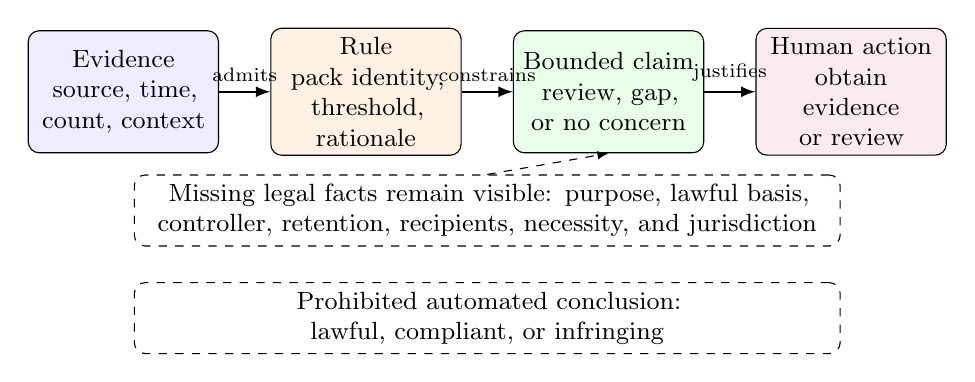
\begin{tikzpicture}[
  node distance=0.65cm,
  box/.style={draw, rounded corners, align=center, text width=0.18\textwidth, minimum height=1.55cm, font=\small},
  note/.style={draw, dashed, rounded corners, align=center, text width=0.72\textwidth, font=\small},
  arrow/.style={-latex, thick}
]
\node[box, fill=blue!7] (evidence) {Evidence\\source, time, count, context};
\node[box, fill=orange!10, right=of evidence] (rule) {Rule\\pack identity, threshold, rationale};
\node[box, fill=green!9, right=of rule] (claim) {Bounded claim\\review, gap, or no concern};
\node[box, fill=purple!8, right=of claim] (action) {Human action\\obtain evidence or review};
\draw[arrow] (evidence) -- node[above,font=\scriptsize]{admits} (rule);
\draw[arrow] (rule) -- node[above,font=\scriptsize]{constrains} (claim);
\draw[arrow] (claim) -- node[above,font=\scriptsize]{justifies} (action);
\node[note, below=1.05cm of $(rule)!0.5!(claim)$] (missing) {Missing legal facts remain visible: purpose, lawful basis, controller, retention, recipients, necessity, and jurisdiction};
\draw[dashed,-latex] (missing.north) -- (claim.south);
\node[note, below=0.45cm of missing] (prohibited) {Prohibited automated conclusion: lawful, compliant, or infringing};
\end{tikzpicture}
\caption{Evidence-to-action conceptual boundary}
\label{fig:conceptual-boundary}
\end{figure}

The model is directional. Evidence constrains which rule can run; the rule constrains the claim; and the claim constrains the action that can be justified. The interface must not reverse this logic by beginning with a desired compliance label and searching for a supporting count. Nor should it allow an action such as reporting an application to imply that the underlying legal question has already been resolved.

Uncertainty enters at each transition. Evidence may be incomplete, a rule may be a research baseline, a claim may omit legally decisive context, and an action may require professional judgement. Rather than compressing these uncertainties into one confidence score, Privacy Lens retains categorical source, explicit missing fields, rule metadata, and textual boundaries. This choice follows the reviewed literature's emphasis on contextual interpretation and calibrated reliance while remaining implementable in a deterministic prototype.

The model also explains the division of evaluation. Admission and replay tests concern evidence. Threshold and pack fixtures concern rules. Projection and screenshot checks concern claims. Participant and professional-review studies would concern actions and reliance. Keeping these layers separate allows the thesis to answer its engineering questions without presenting unevaluated human or legal outcomes as completed results.


\section{Mapping Governance}

The delivered system makes the five GDPR temporal profiles reviewable as rule cards. Each card records the risk assumption, window and combination, cited reference, counterexample, unknown facts, and a non-assurance review state. The review instrument itself is prepared and machine-checked: the packet at \RepoTree{experiments/mapping-review/v1/} contains thirteen atomic items with blinded reviewer fields, an explicit unsupported category, and independence flags. It has not been returned by any reviewer. This documentation is therefore governance evidence rather than independent legal review: the instrument is complete enough to be handed to an independent reviewer, and a missing or stale attestation still prevents a reassuring legal conclusion.

\section{Synthesis}

The literature yields a precise design requirement: a privacy-review system must preserve the boundary between an observation and the authority of the claim made from it. Android research defines the acquisition constraint; regulatory sources define the missing legal context; HCI and accessibility sources define the communication constraint; and rule-system research defines the maintenance constraint. The following chapter converts this model into explicit requirements, design alternatives, and evidence contracts.

\chapter{Requirements and System Design}

This chapter translates the research gap into a design that can be implemented and evaluated. It first defines the product position and release requirements, then compares rejected alternatives, traces the decision lifecycle, specifies the evidence and rule-pack contracts, and maps each design invariant to an acceptance source. This order follows the central dependency of the system: a user-facing claim is valid only when the evidence, rule, and state transitions that produced it remain reconstructable.

\section{Design Objectives and Requirements}

Privacy Lens is designed as a local review instrument. Its output is a structured prompt for investigation, not a legal decision and not a security-enforcement action. The system accepts bounded permission summaries, validates their shape and temporal relationships, applies the active regulation pack, stores the resulting findings locally, and presents the result with its provenance and limitations.

Table~\ref{tab:r11-requirements} defines the requirements used for implementation and evaluation. The table is intentionally concise; later subsections explain why each requirement is necessary and which failure it prevents.

\begin{table}[H]
\centering
\small
\caption{Evaluated-system requirements and acceptance evidence}
\label{tab:r11-requirements}
\begin{tabular}{p{0.13\textwidth}p{0.50\textwidth}p{0.27\textwidth}}
\toprule
ID & Requirement & Evidence \\
\midrule
F1 & Evaluate supported permission summaries deterministically. & Seeded and boundary suites \\
F2 & Preserve source, time window, pack, rule, and missing context. & Type and repository tests \\
F3 & Reject unsafe identifiers, numbers, sources, timestamps, windows, and contexts. & Adversarial tests \\
F4 & Switch only among registered, versioned regulation packs. & Pack registry tests and Settings UI \\
F5 & Separate synthetic demonstrations from device-visible evidence. & Source labels and simulator tests \\
U1 & Provide overview, findings, and settings through stable navigation. & Physical screenshots and UI trees \\
U2 & Communicate severity without colour alone and disclose evidence limits. & Source inspection and physical rendering \\
P1 & Keep findings local, disable Android backup, and request no sensitive runtime permission. & Manifest and installed package inspection \\
D1 & Build a versioned release APK and AAB with a stable package identity. & Release build and device install \\
\bottomrule
\end{tabular}
\end{table}

\section{Design Alternatives and Threat Model}

The model includes malformed bridge values, forged simulator provenance, unsafe numbers, replayed windows, overlapping summaries, unbounded history, misleading empty results, and user over-reliance on authoritative language. It does not defend against a compromised operating system, a maliciously modified application binary, falsified system telemetry, or a legally incorrect pack supplied by a trusted maintainer. Those risks require platform integrity, signing governance, and independent legal review.

\subsection{Selection Rationale}

Several alternative product positions were considered and rejected for specific reasons. On presentation and output, a binary compliance scanner would have to derive purpose, necessity, lawful basis, controller obligations and applicable jurisdiction from permission frequency, and a binary label hides missing evidence, so the adopted three-state model retains a needs-review state, an evidence-gap state and an explicitly limited no-technical-concern state. A single risk score was rejected because a high aggregate count, missing purpose, a synthetic source and a consent contradiction have no common natural unit, and weighting them would introduce assumptions that are difficult to justify and easy to overlook; the system stores contributing signals and renders a reasoned state instead. Treating absence of observations as zero activity was rejected because it conflates a real zero with unavailable acquisition, so the model requires a capability-aware source and reports an evidence gap when coverage is missing. A learned classifier was rejected because the project lacked an independently labelled, representative, legally meaningful data set, and training on store categories, malware labels or developer declarations would answer different questions; a deterministic rule engine was selected because it makes boundary behaviour, missing inputs and change history reviewable, which matches the evidence available here rather than claiming that rules are universally superior.

On where legal meaning lives, embedding GDPR language in interface components would have duplicated content, complicated review and made regional extension risky, since changing jurisdiction would require editing presentation and perhaps persistence logic throughout the application, whereas the pack contract centralises that content and forces the engine to record which pack produced a finding. Choosing a region automatically from device locale or location was rejected because locale does not reliably determine applicable law, organisational establishment, data-subject status or processing context, so automatic selection could present the wrong framework with unwarranted confidence; the design requires explicit selection from registered packs and never collects location to decide which law to discuss. Ingesting unrestricted free-form pack files was rejected as exposing users to misleading sources, malformed thresholds, pack confusion and potentially executable content; the registry admits bundled immutable definitions, and signed declarative distribution may follow once schema, publisher, rollback and review controls exist.

On storage and lifecycle, a cloud account with central evidence storage would create a new repository of sensitive behavioural metadata and require authentication, server security, retention, international-transfer analysis and deletion workflows, so the product is local-first, uses no account and offers local deletion. Keeping a complete raw event history would improve forensic detail but increase sensitivity and resource cost, so the candidate stores bounded findings and the aggregate history needed for current temporal reasoning, and defers event-level acquisition until an authority model, minimisation policy and retention design can be evaluated. Notification behaviour follows the same discipline: repository logic classifies whether a finding is new, has changed state or has escalated and stores that classification with the finding, but no notification channel consumes it in the evaluated build, so this is a prepared extension point rather than an operating feature.

\section{Architecture and Decision Lifecycle}

The selected architecture separates acquisition, admission, temporal preparation, evaluation, persistence, projection, and presentation. Rather than allowing each screen to interpret raw Android data independently, every stage receives a bounded input and produces a state whose meaning is explicit. The following lifecycle, failure, minimisation, and release-gate decisions define how this separation behaves under both normal and adverse conditions.

Figure~\ref{fig:system-architecture} shows the single decision path and the two governance inputs that constrain it. The regulation pack does not receive UI state, and the interface does not bypass the finding record to reinterpret raw evidence. This separation makes source identity and pack identity available at every downstream review point.

\begin{figure}[H]
\centering
\resizebox{0.94\textwidth}{!}{%
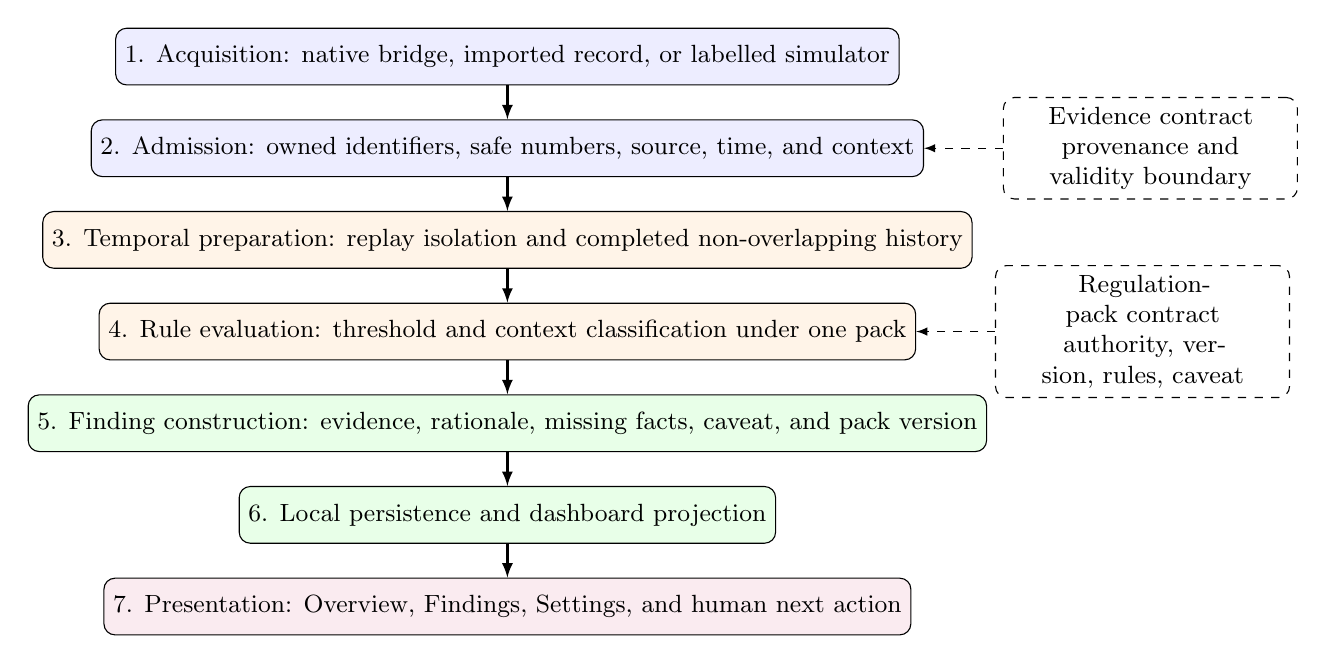
\begin{tikzpicture}[
  node distance=0.43cm,
  stage/.style={draw, rounded corners, minimum width=6.7cm, minimum height=0.72cm, align=center, font=\small},
  side/.style={draw, dashed, rounded corners, text width=3.5cm, align=center, font=\small},
  arrow/.style={-latex, thick}
]
\node[stage, fill=blue!7] (acq) {1. Acquisition: native bridge, imported record, or labelled simulator};
\node[stage, fill=blue!7, below=of acq] (admit) {2. Admission: owned identifiers, safe numbers, source, time, and context};
\node[stage, fill=orange!9, below=of admit] (temporal) {3. Temporal preparation: replay isolation and completed non-overlapping history};
\node[stage, fill=orange!9, below=of temporal] (evaluate) {4. Rule evaluation: threshold and context classification under one pack};
\node[stage, fill=green!9, below=of evaluate] (finding) {5. Finding construction: evidence, rationale, missing facts, caveat, and pack version};
\node[stage, fill=green!9, below=of finding] (store) {6. Local persistence and dashboard projection};
\node[stage, fill=purple!8, below=of store] (present) {7. Presentation: Overview, Findings, Settings, and human next action};
\foreach \a/\b in {acq/admit,admit/temporal,temporal/evaluate,evaluate/finding,finding/store,store/present}{\draw[arrow] (\a) -- (\b);}
\node[side, right=1.0cm of admit] (econtract) {Evidence contract\\provenance and validity boundary};
\node[side, right=1.0cm of evaluate] (pack) {Regulation-pack contract\\authority, version, rules, caveat};
\draw[dashed,-latex] (econtract) -- (admit);
\draw[dashed,-latex] (pack) -- (evaluate);
\end{tikzpicture}
}
\caption{Evidence-bounded system architecture and decision path}
\label{fig:system-architecture}
\end{figure}

\subsection{End-to-End Decision Lifecycle}

The lifecycle begins when the user initiates review, a scheduled worker requests work, or the controlled simulator generates an example. The acquisition component returns candidate records together with a source identity. It must not return a native zero merely because a platform capability is unavailable. Capability failure and an observed zero are different states and lead to different user decisions.

Each candidate crosses the admission boundary as unknown data. The validator checks the package identifier, permission key, count, window, timestamps, source, and optional context without relying on compile-time types. Rejection is structured. The record does not enter temporal history and cannot contribute to a reassuring status. The caller can present the failure as an evidence problem and retain enough diagnostic detail to correct the producer without exposing raw sensitive content unnecessarily.

An admitted record is placed in a key space defined by package and permission. Exact-window replay replaces the prior aggregate. Independent completed windows may be retained for cross-window analysis; overlapping aggregates are not summed. Simulator data remains excluded from accumulated cross-window claims. Retention and a per-key cap bound state. These operations prepare evidence before jurisdictional rules are applied.

The engine receives the selected immutable pack explicitly. It locates the supported rule, calculates daily excess, evaluates burst information where timestamps are available, examines compatible history, and inspects any admitted processing context. The result includes the observed and threshold values, signal types, status, communication priority, rationale, legal or research reference, missing-context questions, and pack identity. The calculation never mutates the pack.

The repository compares the result with the stored finding for the same logical subject. It distinguishes an unchanged state, a new concern, resolution or reversal, and risk escalation. That comparison computes a change classification which is stored with the finding and is intended to govern notification eligibility; as noted above, no notification channel currently consumes it. The comparison also drives the bounded slice written under the versioned repository key. A finding remains attached to its original pack even if Settings later selects another pack.

Projection turns repository records into interface-facing models. It calculates overview totals by state, applies Findings filters, formats source and temporal labels, and exposes actions. Projection should not infer new legal semantics. If a required field is absent, it retains an unknown or evidence-gap presentation. This makes projection testable independently of React components.

Presentation then orders information according to user need. The overview states reach and limitation before the main action. Findings allow scanning by state and inspection of reasons. Settings places pack choice, caveat, simulator, privacy information, and deletion controls in separate groups. Accessibility labels name the action and state rather than depending on icon or colour. Destructive action requires deliberate confirmation where implemented.

The lifecycle ends with user action or explicit non-action. A user may seek a privacy notice, ask a developer for purpose and retention information, repeat review with authorised evidence, or decide that the technical signal does not require immediate attention. Privacy Lens does not contact the reviewed application, change its permissions, or submit a complaint automatically. Keeping the final decision outside the engine preserves human accountability.

Deletion is also part of the lifecycle. The user can clear local findings, and uninstall or platform data clearing removes the application data within Android's boundary because backup is disabled. Export or future synchronisation would create additional copies and must define deletion separately. The current lifecycle intentionally ends at local storage.

\subsection{Failure-State Design}

Failure states were designed as product states rather than exception messages. Acquisition unavailable means the current deployment cannot obtain suitable records; it is not displayed as a completed scan. Invalid evidence means a producer supplied data that fails the contract; it cannot be silently repaired into a normal case. Unknown pack means evaluation is blocked until a registered definition is selected; it does not fall back to the EU pack merely because that pack is bundled.

Storage failure also requires conservative behaviour. If persisted data cannot be parsed or migrated safely, the interface should not mix it with current findings. Recoverable records may be retained after field-level validation, while unrecoverable content should be quarantined or omitted with a visible explanation. Clearing data remains available so the user can recover control. Production logging should report the failure class without printing evidence payloads.

Work scheduling failure is distinct from review failure. WorkManager can defer periodic work because of platform policy, Doze, reboot, or vendor restrictions. The interface should present the last completed review time and source capability rather than imply continuous monitoring. A registered request demonstrates scheduling intent, not on-time execution. Future long-run tests should measure delay and recovery before stronger wording is used.

Partial evaluation is another possibility. Some records may be valid while others are rejected. Treating the batch as wholly clean would hide rejection; treating it as wholly failed would discard useful evidence. A suitable summary reports accepted findings together with the count and reasons for excluded records. The current bounded flows establish structured rejection at record level; richer batch disclosure remains an extension point.

Pack-content failure has two forms. Schema failure is machine detectable and should block admission. Substantive legal error may only be identified by expert review or later correction. Pack provenance, versions, official sources, and historical identity allow the maintainer to issue a successor without pretending earlier findings never existed. The interface can mark a deprecated pack and recommend re-evaluation while preserving the original record.

Network failure is intentionally limited because core review and bundled packs operate locally. Privacy-policy and official-source links may be unavailable, but the application should retain the relevant title and caveat. If remote pack delivery or synchronisation is later added, offline operation and last-known-good behaviour become acceptance requirements rather than optional resilience features.

Visual failure includes clipped localisation, unreadable contrast, focus loss, hidden caveats, and controls obscured by system insets or keyboards. These failures may not appear in logic tests. Rendered screenshot matrices, hierarchy inspection, screen-reader use, font scaling, and device variation are therefore part of the planned evidence. The one-device acceptance check establishes only the candidate baseline.

Finally, misunderstanding is treated as a failure even when the software behaves as coded. If users interpret no technical concern as GDPR compliance, or mistake simulator records for device evidence, the product has failed its communication objective. Participant comprehension and reliance tests are needed to detect that class. The design reduces the risk through terminology and provenance, but does not declare it eliminated.

\subsection{Data-Minimisation Decisions}

The application needs enough evidence to explain a review signal, yet every retained field has privacy cost. Package identifier, permission family, count, time window, source, pack identity, and decision reason form the current minimum for reconstructing an aggregate finding. Optional context is admitted only when supplied for the review purpose. The application does not require account identity, contact lists, precise location content, microphone content, or advertising identifiers.

Counts are stored instead of raw sensor values. A location access finding does not require coordinates, and a microphone access finding does not require audio. This distinction is central: the system reviews evidence that an operation occurred, not the personal data produced by the operation. A future connector should preserve that separation unless a separately approved research question requires content.

Time resolution is also minimised. Aggregate start and end values support window validity, replay, and bounded temporal analysis. Timestamp arrays are accepted for controlled burst evidence, but they should not be collected by default merely because the schema can represent them. The source capability and purpose determine whether additional resolution is justified.

Local-first storage avoids creating a server-side behavioural database. The trade-off is that the user or controlled deployment is responsible for device access and loss, and professional collaboration features are limited. The design disables Android backup so evidence is not restored unexpectedly to another device through ordinary platform backup. This choice should be re-evaluated if enterprise-managed backup becomes a stated requirement.

Bounded history limits denial-of-service and retention exposure. The cap is not a substitute for purpose-based deletion, but it prevents indefinite growth under current aggregate use. Repository slices and clear controls make the lifecycle understandable. Future event-level storage would require stronger indexing, encryption assessment, retention schedules, and selective deletion.

If a notification channel is added, it should carry only the minimum text needed to indicate a changed review state, with detailed evidence remaining inside the application. The evaluated build does not emit notifications, so this is a stated design constraint rather than an observed behaviour. Lock-screen visibility can still expose the existence of a concern, so future production settings should consider notification privacy and user preference. The current evaluation does not claim that every device lock-screen configuration was tested.

External links are used for official materials and privacy documentation instead of embedding broad web content. The application does not send the finding to those sites. Users should be informed that opening a link transfers them to another controller and may reveal ordinary browser metadata. Remote analytics or link tracking would contradict the minimisation posture unless separately justified.

Data minimisation finally applies to evaluation artefacts. Screenshots, UI dumps, log excerpts, and device metadata should avoid unrelated notifications, account names, and installed-application lists. Synthetic demonstrations are preferred for public evidence. Physical records used for thesis acceptance remain scoped to the test application and bounded device session.

\subsection{Requirement Priorities and Release Gates}

Requirements were prioritised according to the harm caused by failure. Evidence admission, provenance, non-verdict language, source separation, replay safety, pack identity, and deletion are release blockers because failure could create misleading privacy conclusions or remove user control. Core navigation, readable hierarchy, package identity, release builds, and absence of sensitive runtime permissions are also blockers for the initial store candidate.

Important but non-blocking research extensions include multi-OEM acquisition measurement, long-duration WorkManager observation, full screen-reader matrices, participant studies, production signing, and independent legal review. They are non-blocking only for the bounded engineering candidate. They become blockers for stronger claims such as public production readiness, accessibility conformance, or validated GDPR guidance.

Optional features include cloud synchronisation, accounts, remote pack updates, application blocking, and learned ranking. These features do not repair current evidence gaps automatically and would introduce substantial security, privacy, or governance work. They should be considered only after the core assurance chain is stable.

The release gate follows dependency order. A source-level failure blocks package evaluation because the binary would not represent an accepted program. A package or manifest failure blocks device acceptance. A device crash or broken primary journey blocks visual promotion. A missing legal or usability study does not turn an engineering check red; it keeps the associated substantive claim explicitly unverified.

This priority model avoids two extremes. It does not delay all prototype learning until every production activity is complete, and it does not allow a successful demonstration to erase unresolved authority or legal questions. Each gate authorises a named next activity. The evaluated candidate supports controlled internal testing and participant-study preparation, subject to the unresolved owner and ethics gates.

\section{Stakeholders and Functional Requirements}

The same evidence contract serves different users, but their decisions and information needs are not identical. Requirements are therefore derived from explicit scenarios before they are divided into functional and non-functional categories.

\subsection{Stakeholders and Usage Scenarios}

The primary user is a person who wants to understand available privacy evidence without becoming an Android or GDPR specialist. This user needs a short account of what was observed, why it deserves attention, what is not known, and what action is reasonable. A second stakeholder is a developer or product owner using the application during internal review. This stakeholder needs reproducible rule identifiers, pack versions, timestamps, and evidence-source labels. A third stakeholder is a privacy or legal reviewer who may use the finding as an entry point into a broader assessment. This stakeholder needs the official source, missing-context questions, and an explicit statement that the application has not reached a legal conclusion.

The first usage scenario is an ordinary review with no prior data. The overview explains the scope before offering a review action. If the bridge returns no admissible observations, the interface reports an evidence gap rather than a clean bill of health. The second scenario is a populated review. Findings are grouped by status and can be inspected individually. The third scenario is learning through synthetic data. The user runs a controlled demonstration, which creates a varied but deterministic set of records marked as synthetic. The fourth scenario is changing legal perspective. The user selects another registered pack, sees its jurisdiction and caveat, and performs a new review without relabelling historical findings. The fifth scenario is withdrawal from the tool itself: the user clears local findings or uninstalls the application.

These scenarios exclude unsupported uses. Privacy Lens is not intended to block another application, intercept network traffic, prove that a sensor callback stopped, obtain evidence by evading platform restrictions, or submit a legal complaint automatically. It does not select applicable law from device location. Defining exclusions is important because a polished interface could otherwise suggest a broader product than the evidence pipeline implements.

\subsection{Functional Decomposition}

The review workflow is decomposed into acquisition, admission, temporal preparation, evaluation, persistence, projection, and presentation. Acquisition produces a candidate summary and a capability statement. Admission checks whether the record can be trusted as a well-formed input. Temporal preparation determines whether history can be combined without double counting. Evaluation applies one immutable pack. Persistence writes findings and migration metadata. Projection converts stored findings into dashboard counts and sections. Presentation renders this projection with actions and caveats.

This decomposition allows each failure to be represented at the correct layer. If the bridge is unavailable, the application should not create a zero-count native record. If a timestamp is unsafe, the engine should not try to repair it silently. If two aggregate windows overlap, the repository should not sum them. If a pack identifier is unknown, the registry should not fall back to whichever pack appears first. If storage migration fails, the interface should avoid presenting stale records as current evidence. The design favours explicit absence over invented continuity.

The simulator follows the same downstream path after acquisition. It is not a separate UI mock that bypasses validation. This is important because a demonstration that constructs presentation objects directly would not test the engine, repository, or projection. Synthetic source identity is introduced at acquisition and persists through every later stage.

\subsection{Non-Functional Requirements}

Security requirements include fail-closed input handling, conservative identifier formats, bounded history, source enumeration, immutable pack definitions, disabled backup, and no sensitive runtime permissions. Privacy requirements include local processing, no remote evidence service, no analytics or advertising SDK, and a clear deletion control. Reliability requirements include deterministic results for identical admitted inputs, replay replacement, pack-specific persistence, and migration from the previous repository schema.

Usability requirements include a clear initial action, a stable three-destination navigation model, non-colour status semantics, concise summaries, optional detail, meaningful accessibility labels, and separation of destructive controls. Maintainability requirements include one authoritative compliance path, typed interfaces, registry-based packs, reusable theme constants, tests for new packs, and removal of duplicate legacy services. Deployability requirements include a stable application identifier, explicit version, current target SDK, release APK and AAB generation, upload-key configuration, privacy-policy content, and documented owner actions.

Performance is treated as a constraint rather than a validated claim. The decision engine operates on bounded in-memory arrays and simple rule lookup. Storage is local and capped per package-permission key. WorkManager is selected for deferrable periodic work rather than exact scheduling. No quantitative battery, long-duration memory, or startup objective is claimed for the evaluated prototype because the available evidence does not cover those dimensions broadly enough.

\section{Evidence and Regulation-Pack Design}

This section specifies the two contracts at the centre of the framework. The evidence contract defines what the engine may know; the regulation-pack contract defines which reviewed rule data may be applied. Admission, temporal isolation, persistence, and abuse controls preserve the boundary between them.

Table~\ref{tab:legal-traceability} prevents the pack's legal references from being mistaken for derivation of its numerical thresholds. The cited provisions motivate review questions. They do not contain daily or per-minute permission limits, and the application cannot infer the legally decisive facts listed in the fourth column.

\begin{table}[H]
\centering
\caption{EU GDPR pack: legal motivation and prohibited inference}
\label{tab:legal-traceability}
\scriptsize
\begin{tabular}{>{\raggedright\arraybackslash}p{0.12\textwidth}>{\raggedright\arraybackslash}p{0.15\textwidth}>{\raggedright\arraybackslash}p{0.19\textwidth}>{\raggedright\arraybackslash}p{0.23\textwidth}>{\raggedright\arraybackslash}p{0.15\textwidth}}
\toprule
Legal anchor & Observed input & Permitted engineering prompt & Facts still required & Prohibited conclusion \\
\midrule
Art. 5(1)(b), purpose limitation & Contacts count and time window & Ask whether access serves an explicit and compatible purpose & Purpose specification, compatibility analysis, recipients, user expectation & Contacts access breached purpose limitation \\
Art. 5(1)(c), data minimisation & Location, microphone, or contacts frequency & Ask whether the observed pattern was necessary and proportionate to the stated function & Function, alternatives, precision, duration, retention, data actually produced & A threshold exceedance was unlawful or excessive \\
Art. 6 and, where applicable, Art. 9 & Declared lawful-basis and special-category context fields & Expose a missing basis or Article 9 condition for human review & Controller assessment, validity of basis, data category, exceptions, withdrawal and objection facts & Processing lacked a valid legal basis \\
Art. 5(2) and Art. 25 & Source, pack version, rationale, missing fields, local controls & Preserve a reproducible prompt and evidence boundary & Wider technical and organisational measures, risk, state of the art, records, governance & The controller demonstrated compliance or the App is certified \\
\bottomrule
\end{tabular}
\end{table}

The legal traceability matrix is deliberately asymmetric. Technical evidence may trigger a question, but a legal proposition is not allowed to flow backwards into the evidence record as if it had been observed. This follows the GDPR and final EDPB guidance while retaining the privacy-engineering distinction between a data action, its context, and the problems it may create \cite{gdpr2016,edpbArticle25,nist8062}.

\subsection{Evidence Schema and Provenance}

The evidence schema is designed around reconstructability. A permission summary includes a package identifier, supported permission key, non-negative safe-integer count, start and end of the aggregate window, source enumeration, and optional processing context. The source is one of the controlled values supported by the application, such as native bridge, imported evidence, or simulator. A free-form source string is rejected because it could allow synthetic data to impersonate device evidence.

Context fields represent what a legal review would need but a permission count cannot provide. Examples include purpose, controller identity, lawful basis, special-category condition, foreground relationship, consent state, retention statement, and sharing information. Their absence does not make the technical record invalid. It changes the finding by adding missing-context questions and preventing a legal conclusion. This distinction separates data-quality failure from legal incompleteness.

A finding contains the admitted evidence plus decision metadata: status, risk, rule identifier, threshold, rationale, regulation-pack identifier and version, official source, evaluation time, and missing-context fields. The schema is intentionally verbose. Storage efficiency is less important than the ability to explain why a result appeared and which assumptions applied.

Provenance also constrains metrics. Simulator precision and recall are computed only for records whose expected labels are part of the controlled generator. Imported or native records do not receive an accuracy label because their legal and behavioural ground truth is unknown. Aggregating these sources into one accuracy metric would create a number with no coherent denominator.

\subsection{Admission and Fail-Closed Validation}

Validation occurs at runtime even though the application is written in TypeScript. Static types protect code paths compiled from known sources, but values crossing a native bridge, storage migration, import boundary, or untyped caller can violate those types. The validator therefore treats each field as unknown until checked.

Counts and timestamps must be finite JavaScript safe integers. This excludes negative values, fractional event counts, infinities, not-a-number values, and integers whose arithmetic cannot be represented exactly. The time window must have a strictly earlier start and a later end. An evaluation timestamp must be consistent with the window. Retention values must be positive and bounded. Package identifiers and permission keys must match conservative patterns rather than merely being non-empty strings.

Context validation follows the same rule. String fields must actually be strings before trimming; booleans must not be inferred from truthy text or numbers. The engine does not coerce a value such as the text false into a Boolean because this can reverse meaning. Unknown source and permission values produce an invalid or review-hold state instead of falling through to a default threshold.

Fail-closed does not mean the application crashes. It means the system returns a safe, explicit result that prevents incomplete evidence from being described as no concern. The UI can then explain which field was rejected or why review cannot proceed. This approach supports both security and diagnosability.

\subsection{Temporal Isolation Model}

Aggregate windows create a double-counting problem. Suppose two records report counts for intervals that overlap. Without event identifiers, the system cannot know whether events in the shared interval appear in both counts. Summing them could manufacture a cross-window threshold. The evaluated implementation therefore aggregates, for the same package and permission, only stored windows that end no later than the candidate window's start. The precision of this statement matters: the comparison is made against the incoming window, not among the stored windows themselves. Two previously stored windows that overlap each other can both satisfy the condition and both contribute to a rolling total. The implementation therefore prevents the tested forms of cumulative amplification rather than every possible overlap. Such a case is reachable in principle---one stored window ending forty seconds before the candidate and another ending thirty seconds before it both pass the test even though they intersect---and no registered fixture currently exercises it. The chapter states the boundary of the guarantee instead of describing the retained history as guaranteed non-overlapping.

Two aggregate windows \(w_i=[s_i,e_i)\) and \(w_j=[s_j,e_j)\) are mutually non-overlapping when

\begin{equation}
e_i \leq s_j \quad \lor \quad e_j \leq s_i,
\end{equation}

and that is the notion used in this chapter when independent aggregates are discussed. The implemented test is narrower: a stored window is admitted for accumulation only when it ends no later than the candidate window's start, so only the first disjunct is evaluated, and it is evaluated against the candidate rather than against the other stored windows. Two previously stored windows that overlap each other can therefore both contribute to a rolling total. This follows from the single-pass design: each incoming window is compared once, forward, against the retained set, and the pairwise comparison among stored windows that a batch reconciliation would require is not performed. Adding it would need either event-level identifiers or a second pass over the retained history, and the evaluated baseline has neither. The condition prevents the tested forms of cumulative amplification without guaranteeing that the retained history is mutually disjoint. Interval handling is likewise mixed: timestamp membership is judged on closed intervals, whereas this cross-window admission test behaves as a half-open comparison, so the notation above describes the intended window algebra rather than every comparison the code performs. Exact replay is detected by equal package, permission, start, and end. The newer replay replaces the stored value rather than increasing the history size or total. This makes processing idempotent for a repeated aggregate export.

Retention uses a monotonic watermark derived from the latest admitted window end for the key. Basing expiry on a newly arrived record's timestamp alone would allow a late or forged old record to move the horizon backwards. Records older than the bounded horizon relative to the watermark are removed. Three qualifications belong with this design statement. The watermark belongs to the in-memory aggregate history rather than to any persisted object, so it describes behaviour within a process lifetime. No dedicated test currently asserts the monotonicity property, so it is reported as a design invariant with source-level support rather than as an executed witness. Each package-permission history is additionally capped at a finite maximum; the cap is a denial-of-service safeguard, not a claim about the maximum legitimate event rate.

Cross-window detection is consequently conservative. It may fail to combine useful but overlapping aggregates, yet it avoids asserting a total that the evidence does not support. Event-level identifiers or disjoint platform buckets would permit a richer model. The current design states the limitation rather than guessing how much overlap occurred.

\subsection{Rule-Pack Contract in Detail}

The common pack contract separates descriptive metadata from executable rule data. Descriptive metadata includes identifier, display name, jurisdiction label, version, official source, effective or review date, and caveat. Rule data binds a supported permission signal to a research baseline, threshold logic, severity, rationale, reference label, and missing-context questions.

The registry is the only route from a persisted identifier to a pack object. This prevents arbitrary downloaded or user-entered text from being executed as a rule. Pack objects are immutable so an evaluation cannot observe a threshold changing midway through a run. The engine receives the pack as an explicit dependency, which makes test fixtures clear and avoids hidden global state.

Pack identity is copied into findings rather than represented only by a current settings value. If a user evaluates under the EU pack, selects the Research Baseline, and later opens an older finding, the finding still displays the EU pack and version. This historical stability is essential for auditability.

The pack contract deliberately does not require every jurisdiction to supply an equivalent article number. A rule can use a provision, principle, official guidance reference, or non-legal research identifier. The UI renders a general reference label and source link. This avoids encoding the assumption that all legal systems share the GDPR's structure.

\subsection{State, Persistence, and Migration}

The privacy context coordinates bridge capability, active pack, loading state, findings, demonstration status, and repository actions. State transitions are explicit: idle, reviewing, completed, and failed or unavailable. The interface disables duplicate actions while a review is running and provides a human-readable result when acquisition returns no evidence.

Three state objects are involved, and they must not be described as one persistence story. Table~\ref{tab:state-objects} separates them.

\begin{table}[H]
\centering
\caption{State objects, retention, and recovery scope}
\label{tab:state-objects}
\scriptsize
\setlength{\tabcolsep}{3pt}
\begin{tabular}{>{\raggedright\arraybackslash}p{0.13\textwidth}>{\raggedright\arraybackslash}p{0.20\textwidth}>{\raggedright\arraybackslash}p{0.17\textwidth}>{\raggedright\arraybackslash}p{0.17\textwidth}>{\raggedright\arraybackslash}p{0.21\textwidth}}
\toprule
State object & What it holds & Retention and horizon & Export, restore, clear & What it does not cover \\
\midrule
Aggregate window history & per package-and-permission window summaries (start, end, count) & bounded to 4{,}096 retained summaries per key; entries older than one day relative to a monotonic watermark are dropped & no export, restore, or clear path; it ends with the engine instance & not durable across process death; the watermark property is in-process and is not witnessed by a dedicated test \\
Temporal observation ledger & per package, normalised observations with type, channel, processing context, destination, evidence kind, timestamp, count, source, and deduplication key & bounded to 10{,}000 observations per package; the horizon is the mounted pack's largest rule window (one hour for the EU pack, twenty minutes for the research baseline) & exported to app-private storage under the mounted pack identity and version; the export is bounded per package but not across packages, so the total snapshot is not globally capped; restore applies a leading 10{,}000-entry bound and rejects the whole snapshot on any schema, pack, version, or field violation & not a general history import; an event outside the horizon invalidates the snapshot at restore rather than being silently discarded; does not restore foreign-version or corrupted state \\
Persisted finding repository & findings as presented, with decision metadata and pack identity & bounded to 100 findings; no expiry & listed, replaced, cleared, and saved through one repository; clearing removes the stored findings and the stored ledger key & not an evidence archive; clearing does not reset already-resident in-memory state in the current process \\
\bottomrule
\end{tabular}
\end{table}

Two consequences of this separation deserve to be stated plainly, because earlier descriptions in the project treated the three objects as one. First, clearing findings removes persisted review records and the persisted ledger key, but it does not reset the running engine, so an aggregate history and a ledger already resident in memory can persist in the current process until that process ends. Second, the ledger's retention horizon is the mounted pack's largest rule window, not a fixed daily horizon; the one-day horizon belongs to the aggregate window history. A reader who merges the two objects will overstate what survives a restart. The export bound and the per-package retention bound are also two distinct constants that currently share the value 10{,}000.

AsyncStorage is used for app-private persistence. The repository key is versioned. On load, older records are normalised into the current schema where safe. Fields that cannot be reconstructed are marked missing rather than invented. A migration should preserve source identity and original timestamps. If a record cannot satisfy current admission rules, it should be excluded from the active projection and surfaced as a migration issue where appropriate.

Clearing findings removes the persisted review records and the persisted temporal-ledger key while preserving the application itself. Pack selection may be retained separately because it is a preference, but the UI states what the clear action affects. The action does not reset in-memory engine state in the current process, as Table~\ref{tab:state-objects} records. That separation is deliberate rather than incidental: the repository is the persistence layer, while the engine is a stateful instance holding its own aggregate history and ledger, so clearing persisted review data does not implicitly tear down a running evaluation. A deployment that requires the two lifecycles to be coupled would add an explicit engine-reset step at the clear action; the evaluated baseline keeps them separate and states the consequence. Android backup is disabled so uninstalling or clearing application data has the expected local-deletion meaning within the platform boundary.

\subsection{Security and Abuse Cases}

The first abuse case is source forgery: a caller marks synthetic input as native. Enumeration and bridge-controlled construction reduce this risk inside the application, although a modified binary is outside the threat model. The second is numeric abuse: extremely large or non-finite counts cause overflow or misleading totals. Safe-integer validation rejects them. The third is replay amplification. Exact-window replacement provides idempotence. The fourth is overlap amplification, addressed by temporal isolation.

The fifth case is history exhaustion. An attacker or faulty source supplies many distinct windows. Per-key caps and retention limit memory growth. The sixth is identifier pollution, where many malformed package or permission strings create unbounded partitions. Conservative formats and supported permission enumeration reject these values. The seventh is pack confusion, where an unknown identifier is presented under a trusted legal name. Registry-only loading and copied pack metadata prevent silent fallback.

The final abuse case is epistemic rather than computational: a user or stakeholder treats a finding as a legal determination. Interface caveats, neutral statuses, official-source links, and missing-context questions reduce this risk. They cannot eliminate it. Training, documentation, and qualified review remain necessary controls.

\section{Temporal Combination Model}

The evaluated implementation adds a narrow temporal inference layer between observation capture and the human-review workflow. Let an observation be $e=(p,t,k,c,s)$, where $p$ is a package-scoped subject, $t$ an observed time, $k$ a normalised observation type, $c$ a non-negative count, and $s$ an evidence source. The domain of $k$ includes permission-relevant data and sensor activities such as location, microphone, contacts, camera, body sensors, activity recognition, media-related access, clipboard reads, device identifiers, backgrounding, and data transfer. It is an engineering vocabulary, not a claim that every Android API call has been observed or legally classified.

A temporal profile $r=(id,W,M,L,q)$ is supplied by the active regulation pack, not by the generic detector. $W$ is the rule-specific positive window length, $M$ is a multiset of required types with minimum counts, $L$ contains the rule-owned legal references, and $q$ is a short rationale. For a candidate time $T$, the detector considers the per-package ledger $E_{p,T,W}=\{e \mid T-W \leq t \leq T\}$. A profile matches precisely when, for every $(k,n)\in M$, the summed count of observations of type $k$ in $E_{p,T,W}$ is at least $n$. No requirement is imposed on the order in which the members of $M$ occur. This makes a combination such as location, activity recognition, and body-sensor access equivalent under every permutation while retaining its observed timestamps and sources as evidence.

Algorithm~\ref{alg:temporal-match} states the admission and matching procedure that the preceding paragraphs describe, at the abstraction level of the model. It shows the sequence of refusals that precede any match, and it contains no step that could emit a legal conclusion. The procedure is deterministic given the admitted observation set and the mounted profile, and every refusal branch returns a typed rejection rather than a default.

\begin{algorithm}[H]
\caption{Fail-closed admission and bounded temporal matching}
\label{alg:temporal-match}
\begin{algorithmic}[1]
\Require raw observation $u$; mounted profile $r=(id,W,M,L,q)$; per-package ledger $E_p$; mounted-pack window bound $W_{\max}=\max_{r'\in\text{pack}} r'.W$
\Ensure a review obligation, or a typed rejection
\State $a \gets \Call{Validate}{u}$ \Comment{identifiers, safe integers, ordered bounded window, closed source vocabulary}
\If{$a$ is a rejection}
  \State \Return \textsc{reject}$(a)$ \Comment{never a default and never a reassuring state}
\EndIf
\State $E_p \gets E_p \cup \{(p, t, k, c, s)\}$ from $a$
\State \Call{TrimToHorizon}{$E_p$, $W_{\max}$} \Comment{drop entries outside the mounted pack's largest window, not the current rule's window}
\State \Call{TrimToCapacity}{$E_p$} \Comment{bounded per-package retention}
\ForAll{candidate times $T$ for $a$}
  \State $S \gets \{e \in E_p \mid T - r.W \le e.t \le T\}$
  \If{\Call{SourceAndPackAdmissible}{$S$, $r$}} \Comment{provenance and pack identity must agree}
    \State $ok \gets \mathbf{true}$
    \ForAll{$(k,n) \in r.M$}
      \If{$\sum_{e \in S} [e.k = k]\cdot e.c < n$}
        \State $ok \gets \mathbf{false}$; \textbf{break}
      \EndIf
    \EndFor
    \If{$ok$}
      \State \Return \textsc{review-required}$(r.id, T, r.W, r.L, \Call{Receipt}{S})$
    \EndIf
  \EndIf
\EndFor
\State \Return \textsc{no-match} \Comment{no temporal alert is emitted; a non-match is not a no-concern finding}
\end{algorithmic}
\end{algorithm}

The formulation avoids a global fixed time threshold. $W$, $M$, $L$, and $q$ are properties of the particular assessment item. The mounted GDPR pack expresses distinct wearable location--health, multimodal biometric-capture, cross-domain-profiling, post-background-media-access, and high-frequency-location profiles; their durations and required observations differ. The profile is only an alerting hypothesis with cited legal context. It is not a conclusion that the processing is unlawful, sensitive in fact, or intended for profiling.

Two boundaries are essential. A match is scoped to one package and a bounded ledger, so an event from one application cannot complete a combination for another. A match does not change the App's access-control outcome. It appends an evidence-bearing finding for human review and retains non-blocking behaviour. These boundaries preserve the distinction between a technical signal, missing contextual facts, qualified legal assessment, and any eventual human action.

\section{Restart and Controlled-Fixture Contracts}

The ledger snapshot carries the package name, pack identifier and version, normalised type, channel, processing context, destination, evidence kind, timestamp, count, source category, and a deterministic deduplication key. At restoration the engine first applies a leading bound of 10{,}000 entries, then rejects the whole snapshot when its schema, pack identity, version, type, time, count, source, or deduplication key is invalid. Two corrections to an earlier description of this behaviour are required. Events outside the mounted pack's maximum window, or later than the snapshot time, are filtered when the ledger is exported; they are not silently discarded at restoration, where such an event invalidates the entire snapshot. Clearing local findings removes the persisted findings and the persisted ledger key, but it does not reset the running engine, so in-memory aggregate history and a resident ledger can survive that action within the current process. The export bound and the per-package retention bound are two distinct constants that currently share the value 10{,}000; this thesis reports them separately rather than as one number. A controlled fixture is generated from the compiled active profile, not from a hard-coded GDPR combination, and must carry both the controlled-demo label and native-bridge source. The release bridge rejects this test route.

\section{Typed Formal Evidence Model}

The formal model uses typed evidence domains rather than claiming a complete legal lattice. Let $E_{tech}$ contain admitted technical predicates, $E_{context}$ contextual and organisational predicates, $E_{source}$ provenance metadata, $E_{time}$ bounded temporal metadata, and $E_{policy}$ the versioned rule and pack identity. These domains map directly to the predicate unions, evidence-source fields, temporal observations, ledger records, and regulation-owned constraints implemented in \RepoTree{src/regulations}.

A compiled rule is $R=(A,C,O)$, where $A$ is a finite set of technical antecedents, $C$ a finite set of required contextual predicates, and $O$ the permitted output \texttt{REVIEW\_REQUIRED}. When $A\subseteq E_{tech}$, the evaluator may emit that review output and records $C\setminus E_{context}$ as missing evidence. The output type contains neither \texttt{LEGAL\_VIOLATION} nor \texttt{LEGAL\_COMPLIANCE}. A non-match emits no assessment and therefore cannot become a compliance finding. Even when the represented contextual predicates are present, the software lacks adjudicative authority and does not model every legally relevant fact.

For states sharing source, temporal scope, and policy identity, $x\preceq y$ means only that every predicate in $x$ is also present in $y$. This is a partial information ordering. No join, meet, legal top, or legal bottom is defined, so the thesis does not call it a lattice. Similarly, temporal behaviour is expressed as executable invariants and state-transition predicates, not First-Order Temporal Logic: matching requires a valid active profile, positive window, required multiset counts, compatible pack identity, admitted provenance, and in-bound timestamps.

The correspondence is executable. Governance tests cover $A$, $C$, and the restricted $O$; information-flow fixtures cover typed reachability without upgrading potential paths to execution; source-admission tests cover $E_{source}$; boundary, permutation, restart, and stress tests cover $E_{time}$; and pack-switch tests cover $E_{policy}$. Passing these tests demonstrates conformance to the declared software semantics, not correctness or applicability of a legal mapping.


\section{Traceability and Evaluation Design}

The architecture is complete only when its requirements can be tested at the appropriate layer. This final section links requirements to evidence, identifies stable invariants, and records how future extensions should renew acceptance.

\subsection{Traceability from Requirement to Evidence}

Every requirement is paired with a planned evidence source. Deterministic evaluation is covered by seeded and exact-boundary fixtures. Provenance preservation is covered by type, repository, and presentation tests. Unsafe inputs are covered by adversarial runtime cases. Pack switching is covered by registry and identity assertions plus Settings rendering. Synthetic separation is covered by simulator-source tests and populated-device screenshots.

Navigation and visual hierarchy are evidenced by UI trees and physical screenshots, while accessibility claims remain limited to source and rendered cues. Local processing and permission minimisation are evidenced by dependency review, merged manifest, and installed-package inspection. Delivery is evidenced by successful release tasks, artefact hashes, package metadata, and installation. The matrix does not list legal compliance or broad user adoption because no test in the current protocol can establish them.

\subsection{Evaluation Strategy}

Evaluation is deliberately layered. Source-level checks establish type and lint conformance. Deterministic tests establish consistency with the published rule specification and adversarial rejection behaviour. Android builds establish package integration. Manifest and package inspection establish requested-permission facts. ADB interaction and screenshots establish bounded physical rendering and launch behaviour. Each result is reported at its own layer; no result is extrapolated into legal compliance or population effectiveness.

\subsection{Design Invariants}

The architecture is governed by invariants that should remain true even when screens, acquisition connectors, or legal packs change. First, no accepted finding exists without an admitted evidence source and bounded temporal scope. Second, no legal or research rule exists without a pack identifier and version. Third, unknown, malformed, or unavailable evidence cannot be translated into a reassuring status. Fourth, simulator provenance cannot be upgraded by persistence or presentation. Fifth, historical findings retain the rule identity used at evaluation time. Sixth, local deletion remains available without requiring an account or remote approval.

These invariants are more stable than component names. A future implementation could replace AsyncStorage with Room, React Native with another presentation framework, or bundled packs with signed declarative packages while preserving the same assurance properties. Conversely, a refactor that keeps every current class name but drops source identity or silent-fallback protection would violate the design. Stating invariants therefore makes architectural review less dependent on incidental implementation structure.

The invariants also guide test selection. Admission tests challenge the first and third invariants. Pack-switch and persistence tests challenge the second and fifth. Simulator and cross-window tests challenge the fourth. Manifest, backup, and clear-data checks contribute to the sixth. This mapping helps maintainers decide which evidence to renew after a change. It also reveals gaps: authentication of an external producer, for example, is not yet an invariant guaranteed by the prototype and must not be implied by the controlled source label.

An invariant can fail through wording as well as computation. If a finding correctly stores evidence gap but the screen headlines the review as safe, the third invariant has failed at presentation. If an export omits the pack version, the fifth has failed outside the repository. End-to-end checks are therefore necessary even when unit tests are comprehensive.

Future release reviews should record each invariant as satisfied, failed, or not evidenced, with direct artefact references. A failed invariant blocks promotion. A not-evidenced item may permit a narrower research build, but its associated claim must remain absent. This practice keeps the product's trust model explicit as functionality grows.



\chapter{Implementation}

This chapter explains how the Chapter 3 contracts were realised in the release candidate. Each implementation section begins with the design problem it resolves and then identifies the code path, state transition, or package fact that supplies the evidence, so that implementation detail is included only where it bears on a research question. The chapter does not repeat the removed health-dashboard, experiment, or scoring features; those components are unrelated to the current research questions and no longer form part of the product architecture.

The implementation has four cooperating domains. TypeScript supplies evidence types, validation, regulation packs, deterministic decision logic, and repository behaviour. Kotlin supplies Android capability reporting and deferrable workers. React Native renders the three-destination review journey. Gradle and the Android manifest define package identity, SDK targets, signing inputs, backup behaviour, and final permission declarations. The sections below follow this dependency order from rule data to delivery artefact.


\section{Rule and Evidence Pipeline}

The core implementation problem is to apply a jurisdiction-specific rule without allowing jurisdiction-specific assumptions to enter validation, persistence, or presentation code. The pipeline resolves this problem through an explicit pack dependency, an unknown-to-admitted runtime boundary, deterministic signal computation, a provenance-rich finding, and a repository that notifies only on meaningful change.

\subsection{Regulation-Pack Implementation}

The EU pack is an immutable TypeScript object identified as \texttt{EU\_GDPR}. It declares the European Union and EEA as its jurisdiction label, cites Regulation (EU) 2016/679 as its version label, and links to the consolidated EUR-Lex source. The pack includes a legal caveat that the automated warning supports accountability review and does not determine infringement.

Three permission families are implemented. Location has a research baseline of 24, microphone a baseline of 8, and contacts a baseline of 4. Each baseline uses a multiplier of 1.5, producing prompt thresholds of 36, 12, and 6 respectively. These values are prototype parameters. They are not extracted from GDPR text, not population estimates, and not represented as legal limits. Their purpose is to exercise an explainable evaluation path and provide deterministic boundaries for testing.

The EU pack supplies a rationale and reference for every permission family. Location directs review toward necessity, proportionality, and documented lawful basis under Articles 5 and 6. Microphone review includes the possibility that special-category material may require Article 9 analysis. Contacts review emphasises purpose limitation, minimisation, and lawful basis. The reference is intentionally a prompt rather than an assertion that the cited provision applies to every record.

Missing-evidence logic is also pack-owned. The EU pack asks for specified purpose, Article 6 lawful basis, controller identity, retention period, and, when special-category processing is marked, an Article 9 condition. If processing relies on consent, consent has been withdrawn, and a positive access count remains, the pack returns its most urgent review status. If required context is missing, it returns insufficient evidence. Otherwise a threshold signal produces review required, while the absence of a signal produces no technical concern for the admitted check.

The Research Baseline pack uses higher prototype baselines of 36, 12, and 6 before applying the same multiplier. It uses region-neutral principles and does not require an Article 6 or Article 9 field. Its caveat explicitly states that it is not law or legal advice. The difference demonstrates that the engine can consume pack-owned rules and missing-evidence logic without embedding GDPR branches in generic code.

\subsection{Runtime Validation Pipeline}

The safe evaluation entry point accepts an unknown value rather than trusting its compile-time annotation. The first check requires a non-array object. The package identifier must be a string between one and 255 characters using a conservative character set. Permission type must belong to the owned set of location, microphone, and contacts. Source, if present, must be simulator, native bridge, or imported. This sequence prevents later operations from assuming properties that have not been established.

The access count must be a non-negative safe integer. The window start and end must also be safe integers, the start must precede the end, duration cannot exceed one day (a window of exactly 24 hours is accepted), and the end may lie at most five minutes beyond the evaluation clock. Restored snapshots receive no such tolerance, so a single out-of-range record invalidates the whole snapshot rather than being trimmed. When event timestamps are supplied, their array length must equal the access count and every timestamp must lie within the audit window. These conditions ensure that peak-rate calculations do not operate on inconsistent evidence.

Processing context is validated field by field. Purpose, controller identity, and Article 9 condition are optional strings. Consent-withdrawn, special-category, and user-initiated values are optional Booleans. Lawful basis must belong to the Article 6 enumeration used by the prototype. Retention days must be a non-negative safe integer. Values are rejected rather than coerced because coercion can change meaning at a trust boundary.

Every rejection returns an explicit code and message with a rejection timestamp. The throwing evaluation method is retained for callers that require an exception, but the application can use the safe result to display a controlled evidence gap. This dual interface allows strict internal use without forcing the UI to recover from an untyped exception.

\subsection{Signal Computation}

After admission, the engine loads the rule for the active pack and computes the prompt threshold

\begin{equation}
T_p=\max\left(1,\left\lceil B_pM_p\right\rceil\right),
\end{equation}

where \(B_p\) is the pack baseline and \(M_p\) is the deviation multiplier. Daily excess is \(\max(0,x-T_p)\), where \(x\) is the admitted count. A daily-total signal is emitted only when excess is positive, so equality with the threshold remains below the signal boundary.

When event timestamps are present, the engine sorts them and evaluates a sliding sixty-second interval. Two indices move monotonically through the sorted array, so peak calculation is linear after sorting. Permission-specific burst limits are 12 for location, 6 for microphone, and 4 for contacts. A burst signal is emitted when the observed peak is strictly greater than the configured limit.

The history key combines package and permission. Previous entries outside the one-day watermark are discarded. An entry with the same start and end is treated as replay and replaced. Only entries ending no later than the current start contribute to the completed rolling total. Overlapping entries stay in bounded history but do not contribute to that total. A cross-window signal is disabled for simulator evidence and requires at least one compatible completed window.

Risk derives from the greatest normalised excess across daily, burst, and rolling dimensions. Ratios below the first threshold remain low; larger ratios map through medium, high, and critical bands. Risk controls presentation priority, while the pack separately controls the compliance-review status. Keeping these concepts distinct prevents a large technical deviation from bypassing missing legal context.

\subsection{Finding Construction and Communication}

The finding identifier combines package and permission so the repository can update a stable subject. Evidence fields contain daily count, peak calls per minute, rolling count, and source. Decision fields contain threshold, excess count, active signals, risk, detection time, regulation identifier and name, legal or research reference, and rationale. Compliance fields contain status, applicable principles, missing evidence, and caveat.

Communication is derived after the finding exists. The title identifies the permission review. The summary translates status and signal identifiers into human-readable language. The recommended action first requests missing evidence; an urgent result suggests pausing processing where appropriate and obtaining human review; other results recommend examining purpose, necessity, and proportionality. A presentation priority is derived from status and risk—urgent only for the strongest status or critical risk, silent for no technical concern, and standard otherwise—and is carried in the finding object. The evaluated build has no notification channel to consume it, so the priority is an ordering for the interface rather than an alert policy.

This construction ensures that UI wording is based on stored decision state. A card is not permitted to infer a legal label merely from colour or excess count. It receives the pack name, source, caveat, and missing context that were produced with the finding.

\subsection{Repository Behaviour}

The repository uses a versioned AsyncStorage key. Listing parses the stored array, replacement writes at most the bounded presentation set of 100 findings, and clearing removes the key. The shipped screens complete a review by replacing the stored presentation set rather than by merging an individual record, so the evaluated write path is whole-list replacement. The latest application context also normalises records created by earlier schemas so that pack identity and evidence fields remain available where they can be reconstructed safely.

Change detection is defined over the stored set. A new finding counts as a change, as do a reversal of active state and an increase in risk rank; a byte-for-byte identical record does not. The classification is stored with the finding so that a future notification channel could act on transitions rather than on every evaluation. No such channel exists in the evaluated build, so the thesis reports the classification as prepared infrastructure rather than as an observed notification outcome or as evidence about notification fatigue.

The decision engine's internal temporal history and the persistent finding repository serve different purposes. Engine history supports signal computation within a running context. Repository findings support user review across sessions. Conflating them would either store unnecessary event aggregates indefinitely or make visible findings disappear whenever the process restarts. Ledger export follows the same separation: the implementation exports the bounded temporal ledger only to app-private storage and tags it with the mounted pack identity and version, so rehydration is not a general history import. The Debug Android module accepts a controlled JSON fixture only when the build flag permits it, verifies its explicit label and generic observation vocabulary, and emits the existing passive-audit event; JavaScript independently refuses the call outside Debug Android. The existing context then processes the emitted event through validation, ledger, mapping, evidence receipt, finding construction, and local presentation, so screen code cannot manufacture a reassuring result.


\section{Product Interface and Accessibility}

The interface translates stored findings into a review journey without introducing new compliance semantics. Rather than exposing every technical field simultaneously, it uses stable destinations and progressive detail while keeping source, pack, and evidence reach close to the status they qualify.

\subsection{Interface Implementation}

The Overview screen has four layers. A brand header establishes identity and provides a direct Settings entry. A high-contrast hero panel explains the evidence-before-conclusions proposition and presents the primary review action. A current-review section summarises needs-review, evidence-gap, and no-concern counts. An evidence-reach card explains whether the native bridge is available and why an empty result is not proof of no access.

The Findings screen is designed for both empty and populated states. The empty state explains what will appear and directs the user back to a review or demonstration. The populated state renders reusable finding cards. Each card shows status, permission, package, source, regulation pack, detected signals, rationale, and missing context. Source and regulation are placed near the result because they alter how the result should be interpreted.

The Settings screen separates preference, explanation, demonstration, and deletion. Pack selection is restricted to registry entries. Selecting a pack displays its jurisdiction, version, description, caveat, and official source. The controlled demonstration is visibly separated from device review. Clearing findings uses a destructive visual treatment and explanatory copy.

The custom bottom navigation uses three equally weighted targets with icon, label, accessibility role, selected state, and sufficient touch area. It replaced the platform tab implementation after physical coordinate and hierarchy evidence revealed ambiguity in the previous navigation setup. Navigation semantics no longer depend on obsolete routes.


\section{Declarative Mapping and Decoupled Insertion}

The temporal profiles that the evaluation exercises are pack-owned declarative data rather than branches in generic code. The constraint follows from C1 and C2: a rule that combines observations over a window must be replaceable without allowing its legal vocabulary to leak into admission, persistence, or presentation. The implementation separates three responsibilities. The regulation pack stores declarative temporal profiles together with its governance metadata. A conversion module validates profile identifiers, supported observation types, positive counts, legal references, rationale, and a bounded non-zero window before compiling profiles into the generic evaluator's representation. The evaluator accepts only compiled rules and package-scoped observations; it imports no GDPR-specific list and remains reusable when another regulation pack is mounted. The governance validator invokes the mapping validator, so a malformed profile fails closed before it can alter a review.

This preserves linkage without hard coupling. The pack owns legal meaning; the mapping compiler is the explicit translation boundary; the temporal evaluator owns multiset matching, canonical ordering, receipt hashing, and bounded-ledger treatment; and the compliance engine owns the finding lifecycle. Swapping the mounted pack changes valid windows and combinations through the same interface. A research-baseline pack intentionally contains a different sensor-fusion profile, demonstrating that the mapping is data-driven rather than a hidden GDPR fallback.

The Android bridge enriches ordinary audit evidence with normalised observation events only when an available bridge API or action can establish a type, channel, source, and non-zero count. It does not infer absent calls, and zero frequency produces no temporal observation. The compliance engine keeps a bounded per-package ledger, validates the active mapping, deduplicates matched evidence, and emits a neutral temporal-cooccurrence finding containing the rule identifier, window, requirements, observed receipt, legal references, rationale, and source classification. The interface exposes these fields as an evidence card, so a reviewer can see the window and combination rather than an opaque severity label.

The limit is as important as the mechanism. The feature reuses the evidence-writing and presentation path already used by the review engine; it neither denies an API request nor terminates an application. An order-independent cluster of observations can justify a question for review, but without purpose, necessity, data-flow, consent, retention, and lawful-basis evidence it cannot safely justify enforcement. Data-driven substitution therefore demonstrates software replaceability and reviewability; it is not evidence that any pack's mapping is legally correct.

\section{Implementation-to-Requirement Traceability}

The implemented system can be traced directly to the Chapter 3 requirements. \textbf{F1}, deterministic evaluation, is realised by immutable pack rules, strict threshold comparisons, explicit signal calculation, and a stable finding identifier. The implementation does not consult wall-clock randomness or network state when deciding a result. Given the same admitted evidence, compatible history, and pack version, the engine produces the same finding semantics.

\textbf{F2}, provenance preservation, is realised by carrying package, permission, source, start, end, observed count, pack identifier, pack version, rule reference, rationale, and missing-context fields into the finding object. Repository replacement preserves these fields, and the Findings screen displays the source and pack near the status. Provenance is therefore not reconstructed from a current setting after the decision.

\textbf{F3}, fail-closed admission, is realised by accepting unknown runtime values and validating their identifiers, numbers, windows, timestamps, source, and optional context before evaluation. Every rejection produces a typed code and timestamp. A rejected record cannot enter temporal history or become a no-technical-concern finding. This mapping is central to the thesis because a permissive default would reverse the intended claim boundary.

\textbf{F4}, registered pack switching, is realised by a closed registry and explicit pack dependency. The engine does not infer a pack from device locale, arbitrary text, or a persisted object. Settings can select only registered identifiers, and historical findings retain the pack that produced them. The non-legal Research Baseline demonstrates switching while its caveat prevents it from being presented as a validated jurisdiction.

\textbf{F5}, simulator separation, is realised through the controlled source enumeration, simulator-owned record construction, exclusion from cross-window evidence, repository preservation, and visible synthetic labels. The simulator exercises the real downstream pipeline, but its values do not acquire device-observation authority when they reach the dashboard.

The usability requirements map to the product shell. \textbf{U1} is realised by Overview, Findings, and Settings, a three-target navigation component, purposeful empty states, and one dominant review action. \textbf{U2} is realised by textual status labels, icons, non-colour distinctions, evidence-reach copy, source and pack chips, and accessibility labels. These implementation facts support inspectable design conformance; they do not substitute for participant or assistive-technology studies.

The privacy and delivery requirements map to the assembled Android package. \textbf{P1} is realised by app-private storage, disabled backup, direct deletion, no evidence server, and removal of inherited external-storage declarations. \textbf{D1} is realised by the stable package identifier, explicit version, current SDK configuration, environment-based upload-key inputs, APK and AAB tasks, branded resources, and installed-package inspection. The QA signing fallback keeps local reproduction possible while remaining visibly distinct from production signing.

This traceability demonstrates why the implementation chapter excludes unrelated legacy features. A component without a requirement, research question, or acceptance source would add maintenance and interpretation risk without strengthening the thesis. Chapter 5 now evaluates each retained path at the source, rule, package, device, and presentation layers.

\chapter{Evaluation and Results}

This chapter evaluates whether the implemented system preserves the evidence boundary defined in Chapters 2 and 3. The protocol separates logical conformance, hostile input handling, temporal state, pack identity, Android packaging, physical interaction, and visual communication. Results are reported before interpretation so that a positive engineering outcome is not silently promoted into a legal, population, or store-approval claim.

\section{Evaluation Overview and Headline Results}

The evaluation separates seven evidence layers: (1) source and specification conformance; (2) deterministic and adversarial rule behaviour; (3) formal properties and curated mutation detection; (4) corpus-scale static and workflow evidence; (5) assembled-package and physical-device integration; (6) rendered UI and accessibility-oriented inspection; and (7) independent human and legal validation. Layers one to six contain the bounded observations reported below. Layer seven remains \texttt{NOT\_RUN}. This separation prevents a passed unit test from being reported as device reliability, human comprehension, or legal validity. Historical receipts remain under \RepoTree{testing-report/}; the final OPPO package and interaction receipt is retained under \RepoTree{testing-report/real-device-9-8-finalize-v1.15.0/}.

\subsection{Evidence Objects, Units, and Denominators}

Table~\ref{tab:evidence-objects} states the unit of analysis that each evidence object supports, and it exists to make unit mixing visible. Counts expressed in different units---seeded logical cases, generated permutations, executed assertions, matched rule events, APK files, package identities, workflow runs, device runs, interface observations, and review-packet items---are not summed anywhere in this thesis, and no two rows may be added together. Where the relation between two objects is not established by a recorded mapping, they are reported separately rather than as one funnel. In particular, the \FDroidCensusN{}-APK static census and the \DevicePackagesN{}-package device denominator are separate populations, and no verified mapping from the former to the latter is claimed.

\begin{table}[H]
\centering
\caption{Evidence objects, recorded scale, unit of analysis, and what each can support}
\label{tab:evidence-objects}
\scriptsize
\setlength{\tabcolsep}{3pt}
\begin{tabular}{>{\raggedright\arraybackslash}p{0.14\textwidth}>{\raggedright\arraybackslash}p{0.23\textwidth}>{\raggedright\arraybackslash}p{0.16\textwidth}>{\raggedright\arraybackslash}p{0.20\textwidth}>{\raggedright\arraybackslash}p{0.19\textwidth}}
\toprule
Evidence object & Recorded scale & Unit of analysis & Supports & Does not support \\
\midrule
Seeded logical campaign & 1{,}000 cases; $(TP,TN,FP,FN)=(800,200,0,0)$ & generated case against a specified oracle & conformance of the engine to the published threshold model & real infringement detection or a population error rate \\
Permutation fixture & six events; 720 permutations & permutation of one effective event multiset & order independence within the stated retention model & global order independence for all states or truncation policies \\
Stress campaign & \StressCorpusN{} corpora; \StressRestartN{} restart; \StressMalformedN{} malformed; \StressAssertionsN{} assertions; \StressRuleMatchesN{} rule matches & generated input, executed assertion, matched rule event & reproducibility and fail-closed invariants on a fixed generated distribution & independent samples, population rates, or performance benchmarks \\
Registered properties and mutants & 9 properties; 9 registered non-equivalent weakenings; 9 reported detections & property and registered weakening & sensitivity to the registered semantic weakenings & a complete mutation score or absence of unmodelled defects \\
F-Droid static census & \FDroidCensusN{} APKs; \FDroidSensitiveN{} sensitive-permission; \FDroidSensitiveNetworkN{} sensitive-plus-network; \FDroidSensitiveBackgroundN{} sensitive-plus-background; \FDroidMultiProcessN{} multi-process & APK file with static manifest and DEX-reference features & composition and processing of the selected corpus & runtime flows, lawful basis, or commercial-store representativeness \\
Device workflow receipts & \DevicePackagesN{} package identities; \CompletedWorkflowsN{} completed; \FailedDeviceWorkflowsN{} retained failures & package identity and workflow run & execution results for this device and fixed procedure & \DevicePackagesN{} devices, \DevicePackagesN{} users, or a complete usage path \\
Recorded failure classes & 26 installer timeouts; 2 no-launchable-activity; 1 package-manager rejection; 1 pre-existing-package protection & retained failure record & the recorded terminal state of the failed runs & causal explanations that were not recorded \\
Post-launch PSS measurements & \PssObservedN{} available of \CompletedWorkflowsN{} completed & measurement on one completed workflow & a descriptive distribution for the measured subset & zero missingness, a memory-leak claim, or a population distribution \\
End-to-end timing measurements & \TimingObservedN{} available of \CompletedWorkflowsN{} completed & recorded workflow duration & the duration of the recorded workflow & per-decision latency of the review engine \\
OEM permission-interface observations & 48 observed; 155 not observed; \FailedDeviceWorkflowsN{} unavailable for failed runs; 31 deny-only notification actions & package run and interface action & the recorded interface boundary behaviour & 31 additional independent applications, or grants and actual use \\
FlowDroid evidence set & \FlowDroidReceiptsN{} receipt; \FlowDroidXmlArtifactsN{} XML artifacts & tool invocation & missing-output handling and adapter interoperability & a successful real-application comparison or algorithm superiority \\
Regulation-mapping review packet & 13 atomic items; independent review not run & review item & preparation of a review instrument & legal approval or inter-rater agreement \\
Single-device release record & one build identity, one device, one interaction interval & installed build on one device & an implementation witness for the recorded scope & cross-OEM behaviour, long-run stability, or accessibility conformance \\
\bottomrule
\end{tabular}
\end{table}

Table~\ref{tab:rq-result-map} then locates the results reported later in this chapter against the four research questions, so that a reader can check that every question receives an answer and that no answer is assembled from a section that does not address it.

\begin{table}[H]
\centering
\caption{Research questions and the sections that answer them}
\label{tab:rq-result-map}
\scriptsize
\setlength{\tabcolsep}{4pt}
\begin{tabular}{>{\raggedright\arraybackslash}p{0.05\textwidth}>{\raggedright\arraybackslash}p{0.42\textwidth}>{\raggedright\arraybackslash}p{0.42\textwidth}}
\toprule
RQ & Principal results in this chapter & Evidence objects used \\
\midrule
RQ1 & Deterministic corpus interpretation; adversarial input results; temporal and replay results; temporal correctness and restart evidence & seeded cases; boundary fixtures; malformed inputs; restart comparisons \\
RQ2 & Accountability and presentation results; visual review method; device interaction protocol & policy fixtures; dashboard projection; UI hierarchy; screenshots \\
RQ3 & Regulation-pack results; cross-pack rejection; retained pack identity in findings; mapping-review preparation & two registered packs; pack-switch fixtures; 13-item review packet \\
RQ4 & F-Droid static census; device workflow denominators and failures; measurement availability; FlowDroid missing output; evidence-object table & corpus records; device receipts; missing measurements; tool receipt \\
\bottomrule
\end{tabular}
\end{table}

\subsection{Source and Rule Verification}

The complete application passed \texttt{tsc --noEmit} and ESLint. The compliance sources were compiled before execution, preventing stale generated JavaScript from being treated as current evidence.

A fixed-seed logical campaign generated 1,000 cases. Eight hundred were expected review signals and 200 were below-threshold controls. The observed confusion matrix was

\begin{equation}
(TP,TN,FP,FN)=(800,200,0,0),
\end{equation}

which gives precision and recall of 1.0000 against the specified oracle. The oracle and engine implement the same published threshold model; this is a conformance and regression result, not an independent estimate of real-world infringement detection. Zero observed errors do not establish a zero population error rate.

Extended suites passed for unsafe types and integers, malformed context, unknown source, permission-key mutation, temporal overlap, adjacency, replay, retention, simulator isolation, dashboard presentation, missing-context disclosure, and regulation-pack identity. The tests confirm the enumerated boundaries. They cannot establish correctness for telemetry the application never receives or for legal interpretation outside the fixtures.

\subsection{Release Build and Manifest Verification}

Gradle completed \texttt{assembleRelease} and \texttt{bundleRelease} with target SDK 36 in the recorded build workflow. The 9 August receipt contains binary hashes for an earlier candidate and is retained as historical build-pipeline evidence; those hashes are not attributed to release \PrivacyLensVersion{}. Two published revisions identify the source line used here: the frozen research baseline is branch \texttt{8-22} at commit \RepoCommitLink{727056c4b29065a4c21ab9bc291c85ca8fa93d5f}{727056c4}, and the mature candidate is branch \texttt{8-24} at commit \RepoCommitLink{225b03476dd863ee79caf56d96f84d52a379daa5}{225b0347}. An undated ``research freeze'' label is avoided because the repository records branch-and-commit identities rather than a single freeze date. The 8 September finalisation rebuilt the release APK and AAB from that source line and recorded their hashes; Play signing and store delivery remain external owner actions.

The reconciled release manifest contained wake lock, boot rescheduling, foreground service, and an application-scoped dynamic-receiver signature permission. Internet, network-state, and legacy external-storage read/write declarations were absent. APK inspection and the installed-package dump reported the same set, with no dangerous runtime permission requested or granted. Android backup was disabled in the application declaration.

\subsection{Physical-Device Evaluation}

The release APK was installed by ADB on one OPPO PERM00 ARM64 device. The installed package reported \texttt{com.zhihengzhang.privacylens}, versionName \PrivacyLensVersion{}, versionCode 16, minSdk 24, and targetSdk 36. Launcher cold start and the overview--findings--settings path succeeded in the bounded 8 September finalisation interval. The filtered crash buffer contained no matching fatal record after that path. This is an observation for one installed build and interval, not a long-run crash-rate estimate.

The three primary destinations rendered at the device's captured application resolution. Coordinate-driven exploration initially appeared to show a navigation-target problem because the physical display and captured application coordinate spaces differed. A bounded coordinate sweep and UI-tree inspection identified the offset; subsequent navigation and custom bottom-bar interaction succeeded. This calibration episode is retained because it demonstrates why raw ADB coordinates must not be interpreted without the target's current window geometry.

The controlled demonstration completed a 50-record synthetic workflow. The populated overview displayed four review items, zero evidence gaps, two no-concern items, and descriptive precision and recall of 100\% for the simulator's known labels. The Findings screen marked the source as synthetic and displayed the EU GDPR pack. These values validate the demonstration path only; they are not device-observation accuracy.

\subsection{Verified Open-Source App-Store Execution}

To test the engineering workflow beyond the project APK, a separate authorised corpus was constructed from the official F-Droid repository. This is an \emph{open-source app-store} corpus, not a closed-source commercial-store sample. The final hash-pinned static census contains \FDroidCensusN{} APKs; the device subset and its exclusion boundary are separately receipt-owned. The corpus boundary and the final static census are recorded under \RepoTree{testing-report/fdroid-open-store-2026-08-22/}, together with the device-batch aggregates. The upstream F-Droid catalogue snapshot from which the corpus was drawn is not part of the published artifact, so corpus composition is reported here from the census itself rather than from a catalogue file. Figure~\ref{fig:census-composition} shows the composition of that corpus, and the overlap warning in its caption is deliberate.

\begin{figure}[H]
\centering
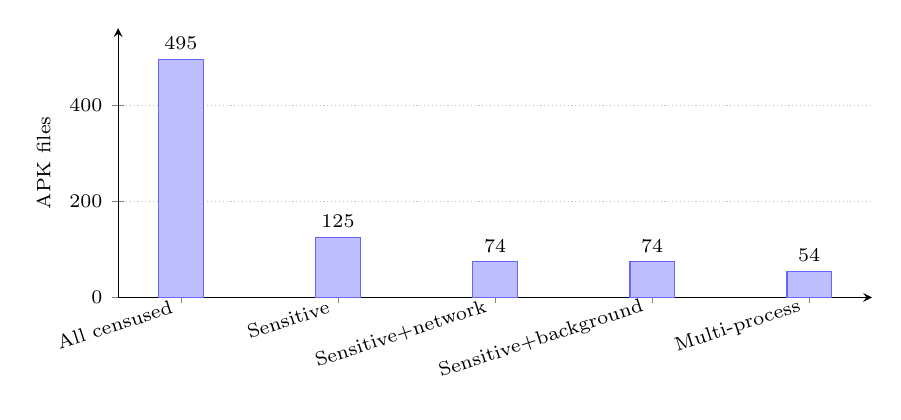
\begin{tikzpicture}
\begin{axis}[
  width=0.92\textwidth, height=5.0cm,
  ybar, bar width=16pt,
  ymin=0, ymax=560,
  ylabel={\scriptsize APK files},
  symbolic x coords={All censused, Sensitive, Sensitive+network, Sensitive+background, Multi-process},
  xtick=data,
  x tick label style={font=\scriptsize, rotate=18, anchor=east},
  y tick label style={font=\scriptsize},
  ymajorgrids, grid style={densely dotted},
  nodes near coords, every node near coord/.append style={font=\scriptsize},
  axis lines=left, enlarge x limits=0.10,
]
% Values match generated-results.tex macros: FDroidCensusN=495,
% FDroidSensitiveN=125, FDroidSensitiveNetworkN=74,
% FDroidSensitiveBackgroundN=74, FDroidMultiProcessN=54.
% Literal coordinates are used because pgfplots cannot parse these macros here.
\addplot[fill=blue!25, draw=blue!60] coordinates {
  (All censused,495)
  (Sensitive,125)
  (Sensitive+network,74)
  (Sensitive+background,74)
  (Multi-process,54)
};
\end{axis}
\end{tikzpicture}
\caption{Static features of the hash-pinned F-Droid corpus. The categories overlap: the sensitive-permission counts are subsets of the censused set, and the network and background counts are not disjoint from one another, so the bars must not be added together.}
\label{fig:census-composition}
\end{figure}

The physical-device runner processed \DevicePackagesN{} distinct package identities over three non-overlapping receipts. It completed \CompletedWorkflowsN{} workflows comprising install, launch, force-stop, and uninstall, and retained \FailedDeviceWorkflowsN{} failures: 26 installer timeouts, two no-launchable-activity cases, one package-manager rejection, and one pre-existing-package protection. No removal failure was observed. The protection is important: a package present before the runner reaches it is neither replaced nor uninstalled, even on the controlled test device.

A final \FDroidCensusN{}-APK static Manifest and DEX-reference census completed without a static failure. It found \FDroidMultiProcessN{} declared multi-process applications, \FDroidSensitiveBackgroundN{} sensitive-permission-plus-background-execution review signals, and \FDroidSensitiveNetworkN{} sensitive-permission-plus-network review signals. These results establish corpus diversity and static review coverage only. They do not establish a runtime source-to-sink flow, controller purpose, lawful basis, necessity, or GDPR infringement. The information-flow model was instead stress-tested through controlled adversarial graphs: obfuscated node identifiers, reflection edges, dynamic runtime-permission evidence, and Binder/Worker cross-process paths preserve a typed review prompt; malformed graph edges fail closed. Its $(TP,FP,TN,FN)=(3,0,1,0)$ result is a fixture-oracle conformance result, not a field estimate.

The final aggregate collected post-launch memory for \PssObservedN{} non-overlapping packages: median PSS was \num{\DevicePssMedianKb} KB with an interquartile range from \num{\DevicePssQOneKb} to \num{\DevicePssQThreeKb} KB. End-to-end workflow time was observed for \TimingObservedN{} completed workflows: the median was \num{\DeviceTimingMedianMs} ms with an interquartile range from \num{\DeviceTimingQOneMs} to \num{\DeviceTimingQThreeMs} ms. Memory was unavailable for 105 of \CompletedWorkflowsN{} completed workflows and timing for 102; these are retained as missing telemetry rather than converted to zero. Across all receipts, the OEM runtime-permission UI was observed but not granted in 48 package runs, not observed in 155, and unavailable for the \FailedDeviceWorkflowsN{} failed runs. A catalog-bound observer separately dismissed 31 exact notification prompts by selecting only the denial control, never a grant control. This shows that the runner preserved the dynamic-permission prompt boundary; it does not establish that each application requested, received, or used a permission. Likewise, the real-app corpus has no independent legal ground truth, so precision, recall, F1, TP, FP, TN, and FN are not computed for it.

\subsection{Public Static-Analysis Baseline}

The frozen FlowDroid 2.15.1 evidence set contains \FlowDroidReceiptsN{} receipt and \FlowDroidXmlArtifactsN{} emitted XML artifacts. The invocation completed without a result artifact. That outcome is retained as missing tool evidence and is not interpreted as zero flows, a true negative, or an application result. The portable adapter is separately exercised with provenance-bound fixtures to show that potential source-to-sink paths can be converted into typed graph evidence while retaining the input identity and receipt hash. A FlowDroid path is a potential static path under the supplied source/sink definition; it is not proof of runtime execution, recipient identity, transfer, purpose, or GDPR infringement. The analytical object and the missing-output boundary therefore support interoperability only, not an accuracy comparison or superiority claim.

\subsection{Formal Properties, Mapping Review, and Accessibility Evidence}

The formal output model distinguishes admitted evidence, typed technical signals, review obligations, and prohibited legal conclusions. Nine registered safety properties have executable witnesses in committed test suites, and the curated mutation campaign reported all nine registered non-equivalent weakenings as detected. The scope of that statement has to be stated carefully, because the recorded evidence is thinner than the word ``detected'' suggests. The documented command \texttt{npm run verify:mutation} copies the compilable sources into an isolated temporary tree, applies one declared source weakening per registered mutant, recompiles that tree, and treats a non-zero exit of the targeted suite as detection. Eight of the nine mutants are exercised through the compiled compliance suite; the ninth is registered against a separate experiment-contract script, which is a weaker binding than the other eight. Each transformation is anchored to an exact source string, and the command aborts if an anchor has drifted, so a mutant cannot be silently skipped; a surviving mutant fails the command.

Two further limits follow from how detection is recorded and how properties are registered. First, the per-mutant receipt stores the detecting test file and a truncated runtime failure tail rather than the failing assertion, and a compilation or load failure would also end in a non-zero exit, so the receipt establishes that the targeted suite failed on each registered weakening rather than that the intended assertion rejected it. Second, the property registry is a static binding: the command that checks it matches a recorded evidence token inside each named test file instead of executing the assertion, so the registry records where a witness lives rather than demonstrating that the witness fails when the property is broken. The pre-correction formulations of the first candidate weakenings were not retained. The project's evolution record lists the surviving candidates, some of which were behaviourally equivalent to the original code and others of which were not witnessed by the cited suite, and the campaign was then corrected to target the actual weakening in each case; because the earlier formulations were not preserved, the initial set cannot be reconstructed item by item, and the thesis does not report a per-item initial survivor count. One property also gained an explicitly anchored order-invariance assertion because its permutation loop had compared every permutation against a reference computed by the same engine. This observed 9/9 result is therefore scoped to the registered set and is not a complete mutation score. It does not prove the absence of unmodelled defects, it does not extend to automatically generated or independently designed mutants, and it does not establish that the assertions are sensitive to defects outside the registered set.

The regulation-mapping review packet at \RepoTree{experiments/mapping-review/v1/} contains 13 atomic items with blinded reviewer fields and an explicit unsupported category, and it specifies at least two independent reviewers. At thesis freeze no reviewer response exists for any item, so independent reviewer judgements and agreement statistics are not available. The review is therefore reported as \texttt{NOT\_RUN}; a prepared instrument, and a specification of how many reviewers it expects, is not a completed review, and no agreement value, legal certification, or completed-review claim is inferred from it. The instrument is nonetheless machine-checked as part of the repository's verification path, so a missing or malformed item cannot pass silently.

On the OPPO device, the current interface exposed non-colour status labels, evidence-source caveats, labelled interactive nodes, and a three-step pause between signal and action. No accessibility service was enabled, and ColorOS did not expose an operable coordinate for committing the extra-large-font preview; the persisted scale remained 0.9. These observations support UI-structure and decision-pause engineering claims only. They do not establish TalkBack traversal, large-font compatibility, participant comprehension, or WCAG conformance.

\subsection{Usability and Trust Assessment}

The product was assessed against three release-candidate questions.

\begin{table}[H]
\centering
\small
\caption{Internal product-screening assessment against the project's release-candidate checklist}
\label{tab:expert-screening}
\begin{tabular}{>{\raggedright\arraybackslash}p{0.19\textwidth}>{\raggedright\arraybackslash}p{0.32\textwidth}>{\raggedright\arraybackslash}p{0.37\textwidth}}
\toprule
Criterion & Supporting evidence & Boundary \\
\midrule
Visually coherent & consistent brand, hierarchy, spacing, cards, iconography, and three-destination navigation on the tested device & one device; no participant preference study \\
Trustworthy & local-first disclosure, source and pack labels, explicit missing evidence, no legal-verdict language & not a legal audit or security certification \\
Interaction feasibility & clear first action, concise summaries, optional details, demonstration, and direct data clearing & expert walkthrough only; no participant or longitudinal adoption measure \\
\bottomrule
\end{tabular}
\end{table}

The screening assessment was performed internally, as the project's single-evaluator walkthrough, on the same handset and installed build recorded above. No independent expert reviewer, third-party assessor, or sample of users took part, and the project record does not separately name the assessor or fix an assessment date. The criteria in Table~\ref{tab:expert-screening}, their supporting evidence, and their stated boundaries are the assessment items used. The outcome is therefore an internal design-conformance judgement rather than an independent evaluation, and it is deliberately narrow: the candidate was judged sufficiently coherent and internally consistent to justify proceeding to participant and internal-track evaluation. The project's desired qualities of ``beautiful, trustworthy, and willing to use'' remain product goals, not measured user outcomes. Stating the assessor's position explicitly matters, because a table titled ``expert assessment'' without an identified assessor would imply an independence that the project does not have.


\section{Engine and Regulation-Pack Results}

The engine evaluation proceeds from nominal threshold conformance to hostile admission, temporal replay, accountability context, and pack independence. This order tests not only whether a rule fires, but whether unsafe evidence is prevented from reaching the rule and whether the resulting meaning survives into presentation.

\subsection{Deterministic Corpus Interpretation}

The confusion matrix compares the engine's active-state decision with the generator's specified expected label:

\begin{equation}
\mathrm{Precision}=\frac{TP}{TP+FP}, \qquad
\mathrm{Recall}=\frac{TP}{TP+FN}.
\end{equation}

The resulting precision and recall of 1.0000 mean that the implementation agreed with the oracle for all generated cases. This supports a regression claim: later refactoring did not alter the expected threshold semantics for the corpus. It also supports a fixture-quality claim: the corpus contains both positive and negative cases and the metric implementation returns the expected counts.

It does not show that a threshold crossing identifies unlawful processing. The expected label is generated from the same documented research model that the engine is meant to implement. Although the oracle is expressed independently of the evaluated result, both are derived from one specification. A defect in that specification could be reproduced consistently. There is no independently labelled sample of real applications or legal cases.

The tests also verify metric edge conditions. Empty samples, all-negative samples, and samples with missed positives must produce finite precision and recall rather than not-a-number or infinity. This matters because a dashboard can otherwise display an apparently precise but meaningless metric when a denominator is zero.

\subsection{Adversarial Input Results}

The initial security cases reject unsupported permission values, not-a-number counts, negative counts, reversed windows, and prototype-like permission keys. Extended cases add unsafe integers and positive infinity. Every such count returns the invalid-count code. Timestamp evidence is rejected when array length differs from count, when an element falls before the start, when it falls after the end, or when it is fractional.

Processing context is attacked through type confusion. Numeric purpose, array controller identity, object Article 9 condition, string consent-withdrawn, numeric special-category, and string user-initiated values all return invalid context. An unknown lawful basis and negative retention period are also rejected. These cases are significant because JavaScript truthiness or an early string operation could otherwise convert malformed evidence into a plausible status or throw outside the controlled error path.

Source validation rejects a forged source. This prevents a caller from using an arbitrary label that resembles an authoritative acquisition path. Package and permission history are isolated: a high-count record for one package cannot make another package active. Histories are also isolated by permission family.

The assertions demonstrate the implemented rejection surface, not complete security. They do not cover a compromised native module, a modified application binary, corrupted AsyncStorage beyond the migration parser, malicious operating system, or every possible Unicode identifier. Security conclusions remain bounded to the enumerated input contract.

\subsection{Temporal and Replay Results}

Burst tests create timestamp arrays exactly at and just above the location, microphone, and contacts limits. At-limit arrays produce no burst signal; one additional event produces the signal. A separate imported-evidence example concentrates 20 location events within one minute and is detected.

Cross-window tests use two below-threshold location summaries. The first remains inactive. When the second begins after the first has completed, their rolling total exceeds the threshold and the engine emits a cross-window signal. The same construction is repeated with adjacent windows to establish that equality between a prior end and current start is admissible.

An overlapping construction uses one interval that intersects the next. The second finding's rolling count remains its own count and no cross-window signal appears. This is the expected conservative behaviour because aggregate evidence cannot identify duplicate events in the overlap. An exact replay is then evaluated twice before a compatible next interval. Rolling total confirms that the repeated window contributed once, not twice.

Simulator histories are excluded from cross-window signalling. The demonstration may still produce a daily or burst signal for a record, but it cannot present accumulated simulator activity as imported temporal evidence. This is a provenance safeguard, not a statistical assumption.

The temporal tests operate in process memory and do not demonstrate persistence of aggregate history across process death. They establish the logic of the current engine instance. A production design requiring durable cross-window evidence would need a versioned evidence-history repository and migration tests separate from the visible finding repository.

\subsection{Accountability and Presentation Results}

A low-count contacts record without processing context returns insufficient evidence rather than no concern. Its communication priority is standard because the absence of legal context warrants review. A low-count location record that supplies purpose, contract basis, controller identity, one-day retention, and user-initiated context still returns insufficient evidence with a standard priority, because the fail-closed governance chain requires a current independent legal-review attestation and verified offline source bytes before any reassuring state is displayed. That is the intended behaviour: the withdrawal of legal context and the unprovisioned review chain both prevent reassurance rather than being filled in by the engine.

A microphone record marked as consent-based, special-category, and accessed after consent withdrawal returns the urgent review status. The fixture does not prove a real GDPR infringement; it confirms that the pack's stated escalation branch is implemented. A special-category microphone record without an Article 9 condition lists that condition among missing evidence. An invented lawful basis and invalid retention value are rejected at admission.

Dashboard projection preserves three different states from the accountability fixtures. Summary totals show one action item, two evidence gaps, and zero no-concern results. Filters surface the expected finding. Every presentation state has both a textual label and marker, ensuring that source-level semantics do not depend on colour alone.

\subsection{Regulation-Pack Results}

The registry exposes at least two packs and recognises only the two expected identifiers. A forged identifier is rejected. The same location audit with a count of 40 is evaluated under both packs. The resulting findings retain different regulation identifiers and different thresholds because each pack supplies its own baseline.

This test is stronger than checking that a dropdown changes text. It passes the same admitted evidence through two independently instantiated engines and inspects the resulting finding objects. The Research Baseline result also contains a caveat stating that it is not law. The test does not validate either pack's legal interpretation; it validates decoupling, identity, and disclosure.

Future pack validation should add a contract suite automatically applied to every registry entry. It should require a unique identifier, version, official-source policy, complete supported-rule set, positive finite baselines and multipliers, non-empty rationale and caveat, deterministic missing-evidence logic, and fixtures reviewed by the responsible domain expert.

\section{Android Artefact and Device Results}

The Android evaluation connects source acceptance to the assembled and installed product. Build reproduction establishes artefact creation; manifest reconciliation establishes package declarations; physical interaction establishes a bounded working journey; and visual review establishes that the principal claim boundaries remain visible on the tested display.


\subsection{Visual Review Method}

Visual assessment considered hierarchy, identity, first-action clarity, state distinction, provenance visibility, limitation placement, empty and populated states, navigation consistency, destructive-action treatment, and overall coherence; aesthetic preference was not scored numerically because no validated participant scale was administered.

The overview succeeded by making the product proposition and review action dominant while keeping the evidence-reach warning in the first viewport. Summary cards used count, icon, label, and colour. Findings showed synthetic source and active pack near the decision. Settings gave the pack caveat and controlled demonstration their own sections. The custom navigation remained legible against the off-white background and used a clear selected state.

The result satisfies a project-defined candidate gate rather than a universal usability standard. One evaluator and one physical device cannot establish willingness to adopt across a population. The strongest supported statement is that the rendered candidate is coherent, presents its boundaries, and is suitable for internal-track and participant evaluation.

\section{Device Workflow Denominators, Failure Classification, and Measurement Missingness}

The device evidence is reported here at the level of the run rather than as a success statistic, because several of the recorded outcomes carry more than one engineering meaning. Of \DevicePackagesN{} distinct package identities presented to the runner, \CompletedWorkflowsN{} workflows completed and \FailedDeviceWorkflowsN{} were retained as failures, so the completed share is $\CompletedWorkflowsN{}/\DevicePackagesN{}\approx87.1\%$ and the retained-failure share is $\FailedDeviceWorkflowsN{}/\DevicePackagesN{}\approx12.9\%$. Table~\ref{tab:device-failures} separates the four recorded failure classes.

\begin{table}[H]
\centering
\caption{Retained device-workflow failures by recorded class}
\label{tab:device-failures}
\scriptsize
\setlength{\tabcolsep}{4pt}
\begin{tabular}{>{\raggedright\arraybackslash}p{0.17\textwidth}>{\raggedright\arraybackslash}p{0.06\textwidth}>{\raggedright\arraybackslash}p{0.34\textwidth}>{\raggedright\arraybackslash}p{0.33\textwidth}}
\toprule
Recorded class & Count & What the record establishes & What the record does not establish \\
\midrule
Installer timeout & 26 & the run ended before installation completed within the recorded timeout & whether the cause lay in the package, the runner, the device, or the network \\
No launchable activity & 2 & the installed package exposed no activity the runner could start & whether the application is unusable for a person \\
Package-manager rejection & 1 & the platform refused the installation & any reason beyond the one the log records \\
Pre-existing-package protection & 1 & a package already present was neither replaced nor uninstalled & that the tooling failed; the protection worked as intended \\
\bottomrule
\end{tabular}
\end{table}

Figure~\ref{fig:device-terminal-states} shows the terminal state of every run and the composition of the retained failures. Installer timeouts account for $26/\FailedDeviceWorkflowsN{}\approx86.7\%$ of the retained failures, so the failure aggregate is dominated by a single recording class whose cause was not captured. The fourth row shows why the table reports terminal states instead of a bare success rate: the pre-existing-package protection is simultaneously an uncompleted workflow and a correct safety behaviour, because it prevents the runner from destroying a package it did not install. Retaining both readings is the honest treatment. No record is relabelled in either direction, and no failure is removed from the denominator. These proportions describe this corpus, this device, and this fixed procedure; they are not a general reliability estimate for the product or for Android applications.

Measurement availability is a second place where the denominator matters. Table~\ref{tab:measurement-availability} reports the recorded values against the completed workflows.

\begin{table}[H]
\centering
\caption{Measurement availability within the \CompletedWorkflowsN{} completed workflows}
\label{tab:measurement-availability}
\scriptsize
\setlength{\tabcolsep}{4pt}
\begin{tabular}{>{\raggedright\arraybackslash}p{0.22\textwidth}>{\raggedright\arraybackslash}p{0.13\textwidth}>{\raggedright\arraybackslash}p{0.13\textwidth}>{\raggedright\arraybackslash}p{0.42\textwidth}}
\toprule
Measurement & Available & Missing & Object that was actually measured \\
\midrule
Post-launch PSS & \PssObservedN{} ($48.3\%$) & 105 ($51.7\%$) & memory of the launched package after launch, on the recorded sampling point \\
End-to-end workflow duration & \TimingObservedN{} ($49.8\%$) & 102 ($50.2\%$) & the complete recorded install--launch--force-stop--uninstall workflow \\
\bottomrule
\end{tabular}
\end{table}

\begin{figure}[H]
\centering
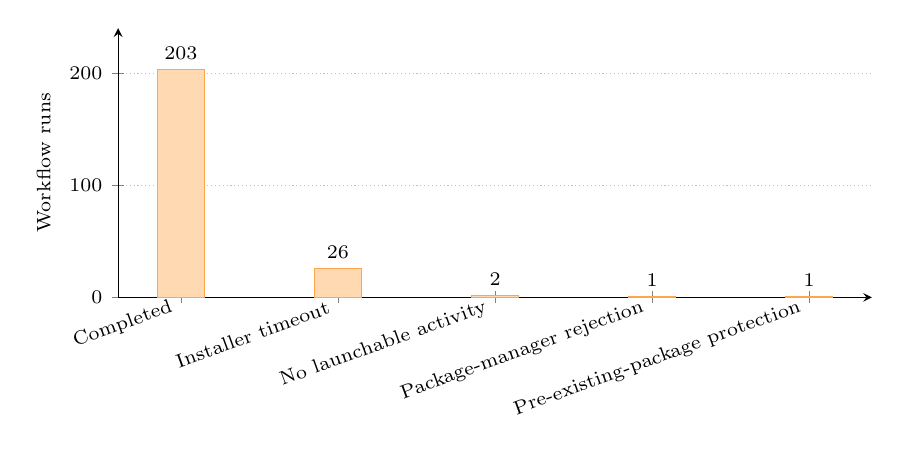
\begin{tikzpicture}
\begin{axis}[
  width=0.92\textwidth, height=5.0cm,
  ybar, bar width=17pt,
  ymin=0, ymax=240,
  ylabel={\scriptsize Workflow runs},
  symbolic x coords={Completed, Installer timeout, No launchable activity, Package-manager rejection, Pre-existing-package protection},
  xtick=data,
  x tick label style={font=\scriptsize, rotate=20, anchor=east},
  y tick label style={font=\scriptsize},
  ymajorgrids, grid style={densely dotted},
  nodes near coords, every node near coord/.append style={font=\scriptsize},
  axis lines=left, enlarge x limits=0.10,
]
% Values match generated-results.tex macros: CompletedWorkflowsN=203,
% FailedDeviceWorkflowsN=30, with the recorded failure classes 26/2/1/1.
\addplot[fill=orange!30, draw=orange!70] coordinates {
  (Completed,203)
  (Installer timeout,26)
  (No launchable activity,2)
  (Package-manager rejection,1)
  (Pre-existing-package protection,1)
};
\end{axis}
\end{tikzpicture}
\caption{Terminal state of every workflow run and the composition of the retained failures. The bars share one denominator of \DevicePackagesN{} package identities; the completed run and the failures are complementary, and the four failure classes sum to the \FailedDeviceWorkflowsN{} retained failures. The last class is simultaneously an uncompleted run and a correct safety behaviour of the runner.}
\label{fig:device-terminal-states}
\end{figure}

The measurement side of the same run is reported separately, because roughly half of the completed workflows have no recorded memory or timing value. The measured subset is therefore reported as a descriptive distribution with its denominator, and the missing values remain missing. They are not replaced by zero, the available subset is never presented without the missing count, and no imputation is used to ``complete'' the series. Because the missingness mechanism has not been identified, the thesis does not claim that the measured subset is a random or unbiased sample of the completed workflows, and it does not assume that the missing values would resemble the measured ones. Two clarifications are required to interpret the two measurements at all. The PSS value describes the launched package's memory after launch; it is not the overhead of the Privacy Lens review engine. The timing value describes the whole recorded workflow; it is not the latency of an individual privacy decision. Repeated operations on the same package identity are not counted as independent device samples.

\section{Temporal Correctness, Restart, and Stress Evidence}

The temporal contribution (C2) is supported by tests written at the abstraction boundary where the claim is made, so that neither the tests nor this chapter silently widens it. Exact-boundary cases exercise timestamps immediately inside and immediately outside a rule-owned window. A six-event fixture is evaluated under all 720 permutations to establish order independence for a fixed subject, pack, effective event multiset, candidate window, and retention set; that qualification matters, because a different arrival order which changes the retained set is not covered by the same result. A seeded 1,000-event burst checks bounded execution rather than presenting a synthetic timing figure as a deployment benchmark. Additional cases verify profile validation, fail-closed rejection of invalid mappings, pack switching, source-receipt generation, integration through the compliance engine, and wording that preserves notification-only behaviour.

Restart behaviour is exercised as a partition, export, restore, and resume comparison rather than as an anecdotal check: for \StressRestartN{} generated cases, the restored temporal evidence receipt must equal the receipt produced by an uninterrupted evaluation. Negative cases reject cross-pack snapshots, expired state, and forged deduplication keys. These results are witnesses inside the stated model. They do not establish completeness against every Android signal, recovery from a corrupted store, or legal accuracy, and the exported ledger is not equivalent to a general history import.

Physical evidence closes a different part of the chain. On 21 August 2026 the then-current source was rebuilt as an offline debug APK and installed by ADB on one OPPO PERM00 device. The UI tree exposed Overview, Findings, and Settings, and the user-visible controlled-device confirmation stated that the fixture was compiled from the active pack, that it was synthetic and advisory, and that it could not inspect or alter another application. Executing it increased the local Findings count from 15 to 16. The new card identified \texttt{\seqsplit{com.zhihengzhang.privacylens.controlled-demo}}, carried the ``Controlled device demo'' provenance label, and rendered the 30-minute, order-agnostic LOCATION, ACTIVITY RECOGNITION, and BODY SENSORS co-occurrence rule once its evidence control was opened. The crash buffer remained empty and the process remained running. This verifies a narrow native-bridge, temporal-engine, ledger, and presentation path. It does not demonstrate a real-world temporal incident, because the fixture neither observed another application nor fabricated sensor activity from the device.

The evidential split is intentional. Automated tests establish temporal rule semantics, mapping substitution, fail-closed behaviour, and non-blocking integration; device inspection establishes installation and one representative interaction path. Neither establishes GDPR compliance, universal Android coverage, legal interpretation, performance on all hardware, or user comprehension.

\subsection{Stress Campaign, Oracle Tier, and Verification Protocol}

To strengthen the evidence beyond the repository corpus, \texttt{\seqsplit{tests/runTemporalStressCampaign.ts}} is executed from a fixed seed over the compiled delivered source. It runs \StressCorpusN{} randomised observation multisets over both registered packs against a count-and-window oracle, \StressRestartN{} random partition, export, restore and resume cases, \StressMalformedN{} malformed-audit cases that require fail-closed rejection with a byte-for-byte unchanged exported temporal ledger, one valid 10,001-entry snapshot that must restore bounded to 10,000 entries, and forged, cross-pack, and expired snapshots that must be rejected. The campaign completes \StressAssertionsN{} assertions and matches the registered temporal rules \StressRuleMatchesN{} times in total, and a stored per-rule breakdown sums exactly to that total over the six registered temporal rules.

Two limits on those figures are stated explicitly rather than left to inference. The assertion count is a count of executed assertions, not of independent samples: it cannot be divided by the corpus size to obtain a population error rate, and it is not decomposable per assertion type from any stored field. The rule-match total is a count of matching events across a generated distribution, not a count of distinct inputs, and it is not a detection rate over the \StressCorpusN{} cases unless per-rule input counts can be shown to be distinct; per-case records were not retained. The generated corpora are therefore counters rather than stored evidence, and a reviewer cannot re-examine an individual case. A non-vacuity guard fails the campaign if any registered temporal rule is never matched, so the corpus cannot silently stop covering one of the rules it declares; the guard covers the registered temporal rules rather than every rule of every pack. Running \texttt{npm run reproduce:thesis-stress} executes the campaign twice and requires both runs to agree on the recorded assertion and rule-match counts before writing a receipt that records the host and the observed totals.

The oracle tier differs between the suites and is named wherever a result is reported. A fixture whose expected value is derived from the same specification that the engine implements yields a conformance result even when the comparison code is written separately, which is the tier of the seeded logical corpus. The temporal rules in the stress campaign are compared against a count-and-window oracle that re-derives counts and windows from each rule's declared requirements instead of calling the production matcher, so its tier is higher within the same model; the oracle nevertheless shares the compiled rule specification, so the comparison is partially independent rather than fully independent. The restart comparison and the order-invariance check are engine-against-engine comparisons of exported receipts, which establishes self-consistency across export, restore, and resume rather than independence from the implementation. Neither tier reaches ecological validity, because the inputs remain generated. Continuous integration runs the enumerated checks from a clean dependency installation, and a release-privacy contract checks that the native controlled method is gated by \texttt{BuildConfig.DEBUG}, with the JavaScript bridge delegating that decision to the native boundary so that an offline debug bundle cannot suppress a valid debug-only test.

Device acceptance remains limited to the actual build, installation, UI tree, screenshot, logcat, and crash-buffer evidence collected for that build. A controlled card is synthetic and cannot be reported as an observed privacy event. Taken together, these results establish reproducibility and the tested fail-closed invariants under the specified generated inputs. They are not a performance benchmark, a proof for every possible input, a legal validation, or field evidence.

\section{Interpretation and Validity}

The final stage asks how much authority the combined evidence supports. It triangulates independent artefacts, examines correlated-oracle risk, interprets metrics, applies the project-defined store-candidate gate, and defines which changes would invalidate the result.

\subsection{Result Boundary}

The evidence supports the claim that the specified code compiles, the rule engine conforms to its fixtures, the Android artefacts build, the final package installs and launches, the main interface renders coherently, and provenance remains visible in the tested workflows. It does not support claims about 24-hour execution, battery cost, memory leaks, unrestricted third-party observation, multiple OEMs, legal compliance, accessibility conformance, production signing, or store acceptance.

\subsection{Evidence Triangulation}

No single method in the campaign was designed to carry the complete acceptance claim. Source inspection is good at confirming constants, branches, labels, and data flow, but it cannot establish which code entered an APK or how a screen rendered. Automated tests execute specified behaviours repeatedly, but their assertions can share assumptions with the implementation. Package inspection observes the assembled artefact, but it cannot prove the meaning of every runtime path. Device interaction observes a concrete installation, but the sample is narrow. The evaluation therefore uses convergence among methods while preserving the scope of each.

Figure~\ref{fig:evaluation-triangulation} presents this assurance structure. Solid arrows connect evidence produced in the study; dashed arrows mark validation that remains external or future. The shape prevents a large logical test count from visually overwhelming the smaller but qualitatively different device, human, and legal evidence classes.

\begin{figure}[H]
\centering
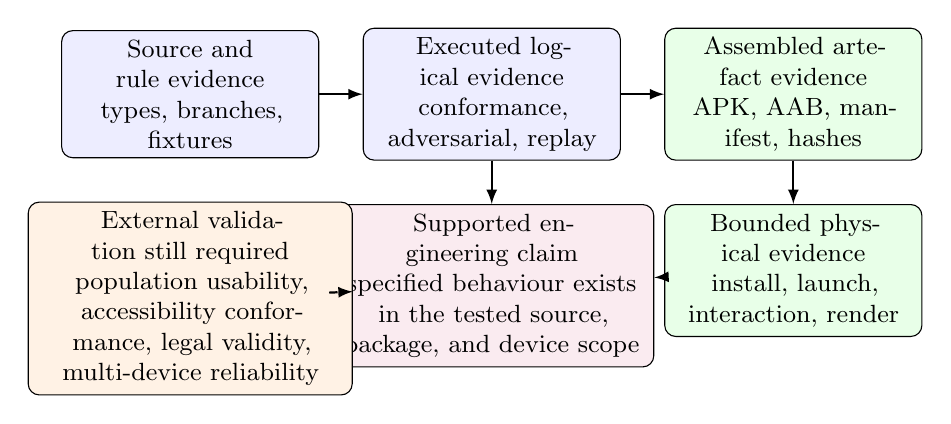
\begin{tikzpicture}[
  node distance=0.55cm,
  evidence/.style={draw, rounded corners, align=center, text width=0.25\textwidth, minimum height=1.25cm, font=\small},
  claim/.style={draw, rounded corners, align=center, text width=0.32\textwidth, minimum height=1.25cm, font=\small},
  arrow/.style={-latex, thick}
]
\node[evidence, fill=blue!7] (source) {Source and rule evidence\\types, branches, fixtures};
\node[evidence, fill=blue!7, right=of source] (tests) {Executed logical evidence\\conformance, adversarial, replay};
\node[evidence, fill=green!9, right=of tests] (package) {Assembled artefact evidence\\APK, AAB, manifest, hashes};
\node[evidence, fill=green!9, below=of package] (device) {Bounded physical evidence\\install, launch, interaction, render};
\node[claim, fill=purple!8, below=of tests] (supported) {Supported engineering claim\\specified behaviour exists in the tested source, package, and device scope};
\node[claim, fill=orange!10, below=of source] (external) {External validation still required\\population usability, accessibility conformance, legal validity, multi-device reliability};
\draw[arrow] (source) -- (tests);
\draw[arrow] (tests) -- (package);
\draw[arrow] (package) -- (device);
\draw[arrow] (tests) -- (supported);
\draw[arrow] (device) -- (supported);
\draw[dashed,-latex,thick] (supported) -- (external);
\end{tikzpicture}
\caption{Evaluation triangulation and claim boundary}
\label{fig:evaluation-triangulation}
\end{figure}

The deterministic tests and source review converge on threshold semantics. Source review identifies the pack-provided baseline, multiplier, daily threshold, burst limit, and source restrictions. Boundary assertions then test values immediately around those decision points. The fixed corpus tests varied inputs at scale. Agreement across these methods reduces the chance that the reported rule differs accidentally from the implemented one. It still does not establish that the rule is a valid legal classifier.

Runtime-boundary tests and presentation tests converge on uncertainty handling. Malformed evidence is rejected at admission, low-context evidence becomes an evidence gap, and presentation projection retains that state. This end-to-end check matters because a correct engine could be undermined if the UI translated an unknown state into reassuring copy. The tests show that selected fixtures preserve meaning through the current projection; screenshot review confirms the principal labels are visible in the rendered flow.

Build logs, output existence, checksums, manifest inspection, installed-package metadata, and physical launch converge on artefact identity. Each closes a different substitution risk. A successful Gradle message without an output file would be insufficient. A local file without a checksum could be confused after rebuilding. Source manifest facts could differ after dependency merging. An installed package could be a stale version. Reading these signals together supports the conclusion that the evaluated handset ran the recorded release candidate.

Visual review and UI-hierarchy inspection also complement each other, because a screenshot shows layout and hierarchy as a person sees them while a hierarchy dump exposes text, bounds and accessibility-node structure; neither replaces screen-reader interaction, large-font testing or participant comprehension.

Triangulation is not vote counting. Where one authoritative check contradicts another, the discrepancy must be resolved rather than outvoted, and greater weight belongs to evidence closest to the released artefact for package claims and to independent human or legal review for substantive claims.

\subsection{Oracle Independence and Correlated Defect Risk}

The main corpus labels are derived from the same published threshold model the implementation is intended to realise. This is appropriate for conformance testing: it asks whether the program implements the specification. It is insufficient for empirical validation because a mistaken specification can yield perfect agreement. The measured 1.0000 precision and recall are therefore implementation-oracle agreement values, not estimates of performance on real legal cases.

Several design choices reduce accidental coupling. The generator records expected polarity directly from its construction, a fresh engine limits cross-case state, boundary cases are written explicitly, and extended tests target properties beyond the main daily-total rule. Nevertheless, developer knowledge shaped both sides. The campaign did not use a separately developed executable oracle, blinded labels, or an external benchmark.

The distinction between what has been done and what has not must be stated precisely here, because a curated campaign of exactly this kind has already been executed. Nine registered, non-equivalent weakenings were applied individually to a copied compilable tree, and the compiled suite failed on every one, as reported above. Three extensions remain \emph{not} done. The first is automatically generated mutants, which would remove the reliance on the author's choice of weakening. The second is independently designed mutants, written by a reviewer who has not read the production engine. The third is property-based generation of many valid and invalid evidence shapes, which would explore inputs beyond the registered corpus while preserving the stated invariants.

Each extension would address a different weakness, and none of them is guaranteed by the 9/9 result. A curated set cannot estimate mutational robustness in general. The registry was revised after the initial execution found candidate weakenings surviving, some of them behaviourally equivalent to the original code and others not witnessed by the cited suite. Because the pre-correction formulations were not retained, the initial set cannot be reconstructed item by item, and this thesis does not report a per-item initial survivor count. The final 9/9 therefore reflects development feedback rather than a blind measure. A detected weakening shows that one assertion distinguishes one wrong implementation; it does not show that unmodelled defects are absent. The same discipline applies in the other direction: a surviving mutant identifies an assertion that executes code without distinguishing correct behaviour, which is a finding about the test suite rather than proof of a program defect.

Two extensions would raise the tier of this evidence: an independently implemented oracle, and ground truth from controlled event traces or independent scenario labelling. Both require work that this thesis does not report, and both are specified as future work in Chapter 7 rather than claimed here.

This distinction explains why the thesis retains the term deterministic corpus rather than benchmark. A benchmark normally suggests comparison against an external reference population. The current corpus is a rigorous regression artefact that protects rule semantics as the code changes. Its value is high, but different from an independently labelled real-world set.

\subsection{Metric Interpretation and Error Analysis}

Precision and recall were included because they expose false-positive and false-negative cells more clearly than accuracy in an imbalanced corpus. The designed 80/20 mixture would allow a trivial always-positive strategy to appear 80 per cent accurate. The full confusion matrix prevents that reading: all 200 controls were negative and all 800 constructed signals were positive under the specified oracle.

The exact totals also make the experiment reproducible. The campaign did not sample a changing external population; it evaluated a fixed generated set. Confidence intervals around the observed proportions would describe repeated sampling from an assumed generator, not uncertainty about the fixed run. More importantly, they would not address specification validity. For this reason the report presents exact agreement and claim boundaries instead of using a narrow interval to imply real-world certainty.

Error analysis remains meaningful even when the main matrix has no disagreements. Adversarial suites reveal categories the primary generator does not represent: unsafe numeric values, prototype-derived identifiers, malformed context, source forgery, temporal overlap, replay, and history isolation. These tests show that corpus size alone is not coverage. A small, carefully targeted case can provide more security evidence than hundreds of additional values drawn from the same safe range.

Reporting for any future field study is specified as future work in Chapters 6 and 7 rather than claimed here: stratification by permission, application category, source authority, foreground status, OEM, Android version and window resolution; inspection of false positives and negatives for common causes; missing acquisition records kept as missing rather than treated as model negatives; excluded cases counted and explained; calibration evaluated separately from discrimination; and denominators defined for operational metrics such as launch success, crash-free periods and rendering smoothness.


\section{Evaluation Synthesis}

The results answer the engineering portion of the research problem question by question rather than as one aggregate score, and Chapter 7 states the answer to each research question. Android evidence connects the accepted source revision to release artefacts, a reconciled manifest, an installed package, and a bounded rendered workflow.

The strongest supported conclusion is therefore a chain rather than a single score. Privacy Lens implements the specified evidence contract, packages that implementation into an installable Android candidate, and communicates its principal limitations coherently on the tested device. Two of the three contributions are carried by that chain: C1 by the preserved evidence and output contract from admission to presentation, and C2 by the bounded temporal, replay, and recovery semantics with their stated conditions and losses. C3 is carried less by any single number than by the way the chain is reported---separate denominators per evidence object, retained failures and missing values, a named oracle tier for each suite, and an explicit statement of what each layer cannot support. The chain stops before legal adjudication, unrestricted acquisition, population performance, broad usability, accessibility conformance, long-run reliability, production signing, and store approval. Chapter 6 examines why those boundaries remain material and which future evidence could move them.

\chapter{Discussion and Limitations}

This chapter interprets the results through the same bounded-claim discipline used in evaluation. It first states what the prototype establishes, then examines technical, legal, human, and operational validity. The discussion does not repeat the result tables; it explains why each remaining limitation changes the authority of the conclusion and which future evidence would be capable of resolving it.

\section{Interpretation of Findings}

\subsection{What the Prototype Establishes}

The prototype shows that a permission-review product can be constructed so that it does not need complete visibility or automated legality in order to make a bounded statement. The core value is not the threshold alone; it is the evidence contract surrounding the threshold. Source, window, pack, rule reference, and missing context make the decision traceable. Fail-closed validation prevents malformed evidence from becoming a reassuring result. The interface then communicates the distinction between an observed signal, a synthetic example, and an evidence gap. Whether that design is in fact useful, or trusted appropriately, to any population remains an empirical question that this thesis does not answer; what is established here is the implementability and internal coherence of the design, not a measured user benefit.

The replacement of a GDPR-specific engine with regulation packs also improves scientific clarity. It reveals which statements belong to generic software and which depend on a jurisdictional interpretation. This supports future extension while making clear that interface compatibility is not legal equivalence.

\subsection{Construct Validity}

The deterministic confusion matrix measures agreement with a defined threshold oracle rather than whether that threshold identifies unlawful processing, and the other evidence types are likewise distinct analytical objects: manifest declarations, DEX references, static paths, runtime traces and policy prompts are each narrowed to what they represent.

\subsection{Internal Validity}

Test fixtures and implementation share parts of the same conceptual specification, so correlated defects remain possible. Boundary suites and the curated 9/9 mutant detections show sensitivity to nine registered weakenings but do not enumerate all plausible defects. The independent mapping packet has been prepared but not reviewed; independent implementation review, completed blinded mapping review, broader mutation generation, and event-level reference traces would further strengthen internal validity.

The simulator is intentionally useful for reproducible demonstration, but it can inflate perceived confidence if its labels are mistaken for field ground truth. The evaluated prototype mitigates this by preserving synthetic provenance through the repository and interface. The remaining risk is user over-reliance on any precise metric; future builds should consider hiding precision and recall outside an explicitly labelled research panel.

\subsection{Device Validity}

Physical evaluation used one OPPO PERM00 device and a short acceptance window. OEM process management, Android versions, accessibility settings, screen sizes, font scaling, languages, network states, and long-run scheduling can change behaviour. No claim is made for 24-hour WorkManager reliability, battery impact, memory leak freedom, or multi-device stability. A release-candidate status at this layer means the tested artefact is coherent enough for controlled store submission work, not that broad compatibility is established.

The ADB coordinate calibration problem also illustrates a methodological limitation: automated interaction evidence depends on the relationship between physical display coordinates, application-window bounds, navigation bars, and screenshots. The 24 August record anchors application actions to captured UI nodes, but the attempted extra-large-font setting could not be committed on ColorOS and no screen reader was enabled. Future UI automation should retain resource identifiers, window geometry, font state, and enabled accessibility services with every run.

\subsection{External Validity}

The \FDroidCensusN{}-APK census provides heterogeneous, hash-pinned open-source artifacts, while the \DevicePackagesN{}-package runner retains its complete eligible denominator and failures. F-Droid remains an open-source repository with its own publishing and maintenance selection effects, and the device subset is constrained by the frozen execution receipts. Neither sample supports prevalence claims for all Android applications, commercial stores, countries, users, or alleged infringements.

\subsection{Ecological Validity}

Static capability and potential source-to-sink paths do not establish executed behaviour in ordinary use. Conversely, a bounded launch workflow samples only the states reached during that run. The current evaluation therefore preserves a distinction among packaged capability, potential static flow, observed device workflow, and policy review prompt; field behaviour would require authorised event-level observation under a separately approved protocol.

\subsection{Legal and Regional Validity}

The GDPR pack maps technical signals to questions motivated by official provisions \cite{gdpr2016}. It cannot determine controller identity, processing purpose, lawful basis, Article 9 condition, necessity, proportionality, consent validity, data-subject expectations, retention, recipients, safeguards, or jurisdiction. The application's output is therefore an accountability aid. A qualified reviewer must examine the underlying processing and applicable law.

Adding another regional pack requires more than translation. The maintainer must identify scope, legal authority, effective date, regulated actors, exceptions, remedies, and concepts that have no GDPR analogue. Each pack needs independent legal sign-off, versioned fixtures, source preservation, localisation review, and an update policy. The current Research Baseline pack is not evidence that a second legal regime has been validated.

\subsection{Human Validity}

The redesigned interface applies recognised accessibility and usability principles \cite{wcag22,androidAccessibility,iso924111}, and the rendered evidence supports a bounded engineering assessment of labels, touch targets, evidence caveats, and the pause between signal and action. However, conformance-oriented inspection cannot establish comprehension, efficiency, satisfaction, trust calibration, or willingness to continue using the product, and Chapter 5 records which accessibility evidence is still missing. Those gaps are required to be closed before making an accessibility-conformance or user-adoption claim.


\subsection{Interpreting the Engineering Result}

The evaluation is strongest when read as a chain of bounded claims rather than as one pass or fail judgement. At the innermost layer, unit and integration tests show that a specified input produces the specified state transition. At the next layer, release assembly and manifest inspection show that the tested TypeScript is incorporated into an installable Android artefact with the recorded package properties. Physical-device interaction then shows that selected routes render and selected controls respond on one hardware and operating-system combination. No layer automatically establishes the next: a correct function may be absent from a package, an installable package may render poorly, and a coherent interface may still be misunderstood by users.

This layered reading prevents a common reporting error in prototype research: promoting evidence because several individually positive checks appear together. Ten successful checks are not equivalent to one check of a broader proposition. A passing threshold test and a successful device launch, for example, do not jointly prove that the threshold represents unlawful processing; they establish two different facts, one logical and one operational. Privacy Lens therefore records evidence by claim type. The report may look more cautious than a conventional demonstration, but it is more useful to a maintainer because it shows which additional study could change a conclusion.

The phrase ``initial store-submission engineering candidate'' is deliberately narrow. It means that the repository can produce the expected release formats, that the product has a coherent user journey and disclosures, and that no known in-scope engineering defect makes controlled submission work irrational. It does not mean that the application is signed with the owner's production key, that a store has reviewed its declarations, or that the legal mappings have been approved by counsel. Separating these meanings matters for privacy software because a polished security or compliance interface can borrow authority from the domain even when its evidence is limited.

There is also a difference between absence of an observed failure and affirmative evidence of a desirable property. No crash during a short device session is evidence about that session, not positive evidence of long-term stability. A small memory range across a few restarts is a useful anomaly check, not a leak proof. No sensitive runtime permission in the merged manifest is a strong package fact, but it does not by itself prove that every future acquisition connector will remain privacy preserving. The evaluation uses explicit negative claims to preserve these distinctions.

The result should therefore be understood as a reproducible decision point. A future reviewer can rebuild the same revision, inspect the same rules and fixtures, and ask whether later evidence warrants promotion from one claim class to another. That property is more durable than a one-time declaration of readiness. It converts the thesis from a retrospective narrative into a maintainable assurance record.

\section{Technical Validity Boundaries}

The central technical limitations concern the authority of acquisition, the meaning of prototype thresholds, temporal aggregation, and the governance of rule data. These issues are grouped because each can make a deterministic output reproducible while still leaving its real-world interpretation uncertain.

\subsection{Acquisition Authority and Observation Quality}

The largest external-validity constraint is not the visual interface or the threshold arithmetic; it is the authority and completeness of the observation source. Android deliberately limits one ordinary application's access to sensitive information about other applications. Privacy Lens does not bypass that security model. The current native bridge and imported-record contracts can carry observations when an authorised deployment supplies them, while the simulator supports deterministic explanation and testing. The prototype must not imply that installing it from a public store grants unrestricted historical visibility.

This constraint affects every downstream conclusion. An apparently quiet history may mean that accesses did not occur, that the selected API does not expose them, that an OEM shortened retention, that the collection job was delayed, or that the current deployment lacks authority. These explanations are not interchangeable. The evidence schema therefore includes source and time-window fields, and an evidence-gap state is preferred when acquisition sufficiency is unknown. A ``no technical concern'' result refers only to accepted records, not to all activity on the device.

Observation quality has at least five dimensions: coverage (which applications, operations and intervals are visible), resolution (event-level or aggregated), timeliness, integrity (whether records can be altered, replayed or reordered), and semantic fidelity (whether the operation label corresponds to the personal-data behaviour under review). A future connector should publish a capability document addressing all five, because merely conforming to the TypeScript shape is insufficient. Aggregate records trade context for storage — ten accesses could be ten user-requested refreshes or repeated background tracking, and a total cannot distinguish them — so the acquisition design must minimise collected fields, bound retention and protect local storage. More data is not automatically a more privacy-preserving audit.

An authorised enterprise or research deployment could improve coverage through device-owner controls, instrumented test applications or controlled firmware, but each option changes the population to which the findings apply, so evaluation reports must name the authority model rather than treat all Android evidence as equivalent. The validation programme that would turn coverage into an empirical statement is specified in Chapter 7.

\subsection{Threshold Meaning, Calibration, and Decision Error}

The implemented baselines and multipliers are transparent prototype parameters, as Chapter 3 records. Transparency makes a rule reproducible without making it representative: a location threshold can be inspected and tested exactly, but its normative meaning depends on application category, user action, service duration and declared purpose, so a navigation application and a static calculator cannot be judged by the same behavioural expectation merely because both run on Android.

False positives and false negatives also have asymmetric consequences. A false positive may alarm a user, damage confidence in a legitimate application, and contribute to warning fatigue. A false negative may reassure the user or reviewer despite activity that deserves investigation. The appropriate balance is not a purely mathematical optimisation because the costs depend on use context. The current design therefore avoids converting a below-threshold result into a compliance statement and avoids converting an exceedance into a violation verdict.

The calibration target must be explicit, because optimising agreement with human reviewers is not the same as predicting store-policy enforcement, detecting malware, or identifying GDPR accountability questions; each target requires different labels and evidence. Privacy Lens targets review prioritisation — a defensible prompt for further examination — which supports conservative wording and structured missing-context questions rather than a binary compliance classifier. The sampling frame, annotation protocol, multi-scale parameter governance and reporting stratification that a calibration programme would need are specified in Chapter 7.

\subsection{Temporal Evidence and Replay Semantics}

The failure modes of time-windowed evidence, and the controls the engine applies to them, are set out in Chapter 3. Two consequences belong in the discussion rather than in the design chapter. The controls specify how the engine behaves under replay without creating event-level identity where none exists, so partially overlapping aggregates cannot always be reconciled; and the conservative response — declining cumulative interpretation when independence cannot be established — trades sensitivity for the avoidance of manufactured precision. Retention follows the same reasoning: keeping only the most recent records bounds memory and reduces local exposure, yet an arbitrary truncation point can remove context needed for a decision, so the history limit is an engineering safeguard rather than a legal retention determination. The temporal properties the registered suite should additionally cover, and the connector designs that would strengthen deduplication, are listed in Chapter 7.

The broader lesson is that time is part of the evidence contract, not metadata attached after classification. A risk statement about repeated behaviour is only as defensible as the window relationships used to compute it. Making those relationships visible helps reviewers distinguish sustained behaviour from an artefact of aggregation.

\subsection{Regulation-Pack Governance Beyond Software Modularity}

The replaceable pack contract solves a software architecture problem: it prevents jurisdiction-specific references, prompts and thresholds from being scattered across screens, storage and native integration code. It does not solve the institutional problem of deciding what a pack should say, because a pack can be syntactically valid and legally misleading. Governance therefore has to be paired with the architecture on two fronts.

The first is admission. A pack must name its jurisdiction, regulated context, legal instruments, effective date, intended users and exclusions; distinguish binding provisions from regulator guidance and from research heuristics; and link each technical condition to a review question plus the missing facts that prevent automated legal determination. Legal review must be independent of the developer who encoded the rule, must cover citation accuracy, applicability, exceptions, terminology and translations, and must attach to a specific pack version and date. Technical admission then validates identifiers, semantic versions, rule uniqueness, supported evidence fields, bounded parameters, localisation completeness and fixture coverage, and the registry rejects an unknown or malformed pack rather than falling back silently to a default. Chapter 3 records the contract itself; Chapter 7 lists the deprecation, rollback and offline-recovery machinery that a downloadable pack would additionally require.

The second is regional variation. Concepts such as controller, covered business, sensitive information, consent, sale, sharing, child or data localisation do not map one-to-one, and enforcement actors and private rights differ, so a common model must carry generic evidence and review primitives while letting packs declare jurisdiction-specific questions; forcing every regime into GDPR terminology would produce superficial flexibility and substantive error. Localisation is likewise more than translating strings: it combines legal-language review, plain-language review in the user's locale, and rendered interface testing, and the interface must identify both the selected region and the pack version. The Research Baseline pack illustrates the disclosure pattern the thesis relies on — switching rule sets while preserving identity, without masquerading as a validated regional law.

\section{Human, Ethical, and Operational Trust}

The product's credibility depends on more than a correct rule. Users must understand the status, the reviewing application must minimise its own privacy and security risks, research evidence must be collected responsibly, and release claims must match the package that is actually distributed.

\subsection{Trust, Comprehension, and Willingness to Use}

Visual coherence is necessary because users make rapid judgements about whether a privacy tool is maintained and safe. Consistent typography, restrained colour, stable navigation, and plain-language hierarchy reduce avoidable friction. They are not sufficient for trustworthiness. A visually polished product can be more dangerous if polish causes users to accept unsupported conclusions. Privacy Lens therefore treats calibrated trust, rather than maximum trust, as the design objective.

Calibrated trust means that confidence changes with evidence quality. A native or authorised imported observation can be described according to its documented capability. A simulator record must remain labelled synthetic. Missing purpose or lawful-basis context must remain visible even when the numerical signal is normal. The interface should make the most important limitation available at the decision point, not bury it exclusively in a policy page.

Willingness to use has several components. Initial adoption depends on a credible value proposition and low setup burden. Continued use depends on whether findings arrive at useful times, whether repeated alerts are suppressed, whether explanations support action, and whether local data controls behave predictably. Recommendation to others may depend on institutional endorsement, independent review, and evidence that the tool does not create new privacy risks. A short expert inspection can assess obvious barriers but cannot establish these behavioural outcomes.

A participant study should therefore use realistic tasks rather than preference ratings alone. Participants could identify the source of a finding, compare two risk states, explain why a low-count record is not a compliance certificate, switch regulation packs, clear local evidence, and decide what follow-up information is needed. Measures should include completion, error, time, comprehension, perceived workload, appropriate reliance, and confidence. Interviews can reveal whether terms such as evidence gap or technical concern match users' mental models.

The sample should include ordinary Android users, privacy-aware users, accessibility participants, and professional reviewers. Their goals differ. Ordinary users may need a concise decision path; professionals may need exportable provenance and exact rule details. Accessibility participants may expose focus order, verbosity, contrast, magnification, or motor-control barriers that visual review misses. The study should avoid treating one group's preference as universal.

Longitudinal testing is necessary for notification design. A single session cannot reproduce fatigue or habituation. A multi-week study could compare immediate alerts, daily summaries, and state-change-only notifications. It should record dismissals and follow-up actions while avoiding collection of unnecessary behavioural telemetry. The hypothesis is not that fewer notifications are always better, but that each interruption should correspond to a meaningful change.

Trust measures also need a correct-answer component. Asking whether participants trust the application can reward unjustified confidence. Better evaluation presents cases with strong evidence, synthetic evidence, missing context, and malformed input, then tests whether confidence tracks those differences. An effective design should sometimes cause the user to withhold judgement. That is a successful outcome for an evidence-bounded review tool.

\subsection{Privacy and Security of the Reviewing Application}

A privacy-review application can itself become a source of sensitive data. Permission histories may reveal health routines, mobility, communication, or working patterns even when they contain no content. Application identifiers can expose relationships or interests. Findings and notification text may be visible to other people with physical access to the device. The product's local-first design reduces network disclosure, but local processing is not automatically risk free.

The current package requests no sensitive runtime permission and disables Android backup. These are valuable minimisation facts for the evaluated build. The application also provides a clear-data control and does not require an account. Future connectors could change this profile. Every new acquisition or synchronisation feature should therefore trigger a new data-flow inventory, manifest reconciliation, threat review, privacy notice update, and store declaration review.

At-rest protection should be proportionate to the threat model. Platform sandboxing protects data from ordinary applications, while device compromise, debug builds, rooted environments, and unlocked backups present different risks. If future deployments store event-level histories or legal annotations, encryption and key lifecycle may become appropriate. Encryption does not eliminate exposure through rendered screens, notifications, logs, or exported files, so those channels also require controls.

Logging is a frequent source of accidental disclosure. Production builds should avoid writing raw evidence, application inventories, or legal-context notes to Logcat. Crash reports, if introduced, should be opt-in where required, minimise payloads, document processors and retention, and avoid attaching the evidence database. Analytics should not be added merely to measure engagement; a privacy tool carries a higher burden to justify behavioural tracking.

Pack supply-chain risk must also be considered. A malicious or compromised pack could present alarming text, suppress review, or direct users to unsafe resources even without executable code. Declarative schema restrictions, signed distribution, trusted publisher identities, URL allow-lists where appropriate, and human review reduce this risk. Bundled packs should be covered by the same source-control and release-review process as application code.

Abuse scenarios include importing fabricated evidence to defame an application, replaying old records as current, selecting a misleading jurisdiction, and showing a screenshot without its source label. Privacy Lens addresses some of these risks through provenance, timestamps, pack identity, and replay controls. It cannot authenticate every external producer in the current prototype. Export formats should preserve those fields and should state that the document is a review artefact rather than a regulator finding.

Security maintenance is part of store readiness. Dependencies, Android target requirements, signing keys, build provenance, and vulnerability disclosures require ongoing ownership after submission. The present thesis records a reproducible snapshot; it cannot guarantee that the same dependencies remain appropriate later. A release process should include dependency review, secret scanning, reproducible build records, and an incident contact before the product is distributed broadly.

\subsection{Research Ethics and Responsible Evaluation}

The safest current evaluation uses synthetic or controlled evidence because real permission histories can expose third-party and participant behaviour. Synthetic data provides precise ground truth and repeatability, but it must be labelled so screenshots and metrics are not mistaken for field evidence. The simulator label is therefore an ethical as well as methodological control.

A future participant or device study would require informed consent describing what is collected, why it is needed, how long it is retained, who can access it, and how withdrawal operates. Researchers should avoid collecting unrelated application inventories or fine-grained histories when controlled test applications can answer the research question. Test accounts and scripted actions should be preferred for validation of acquisition correctness.

The legal subject matter creates an additional risk of participant misunderstanding. Study materials should explain that findings are prompts and that the research team is not providing individual legal advice. Participants should not be encouraged to confront application developers or change essential device settings solely because of a synthetic warning. Debriefing should clarify which cases were fabricated and how the evidence boundaries work.

Reporting should include failed runs, missing observations, exclusions, and changes made after pilot testing. Selectively presenting only coherent screenshots would exaggerate maturity. The repository's separation of logical, package, physical, and visual evidence provides a structure for ethical reporting because each claim can be tied to its acquisition method.

If external legal experts annotate cases, their independence, jurisdiction, instructions, and disagreement process should be recorded. A single expert opinion is valuable but should not be transformed into universal ground truth. Where reasonable interpretations differ, the pack can present the ambiguity as a question rather than forcing a binary label.

Finally, public release creates responsibilities to people who were not research participants. Store text and onboarding must not imply regulatory endorsement. Support channels should handle correction and deletion questions. Pack updates should communicate material interpretation changes. Responsible deployment is therefore a continuing governance activity, not the final administrative step after technical acceptance.

\subsection{Store and Operational Readiness}

The repository contains target-SDK configuration, AAB output, privacy-policy content, a stable package identifier, branded assets, and a store checklist. Google Play nevertheless requires owner-controlled signing and console information, including a Data safety declaration and current policy compliance \cite{playDataSafety,playTargetApiLevel}. The present AAB uses a QA signing fallback when no upload-key environment is provided. Public submission therefore remains blocked on an upload key, HTTPS privacy-policy publication, support contact, final listing content, screenshots selected for the listing, console declarations, internal-track testing, and store review.

\section{Temporal-Alert Limits and Next Validation}

Temporal co-occurrence is necessarily an incomplete proxy. A combined location, sensor, or transfer pattern may be benign, expected by the user, technically misclassified, partially observed, or governed by a lawful purpose not present in local evidence. Conversely, an actual high-risk flow can evade this prototype when it occurs outside a profile's window, uses an unsupported interface, is hidden by platform restrictions, or lacks observable bridge evidence. The bounded ledger intentionally trades historical completeness for local resource control. These are reasons to preserve uncertainty and notification-only operation, not reasons to silently broaden a rule.

Future packs should be authored through controlled legal and engineering review, with versioned source material, traceable interpretation notes, fixtures for matches and non-matches, and a staged rollback path; the rule author rather than the generic engine must set and justify each window and required combination, and pack loading must keep validating the converter boundary so that unsupported observation types, empty legal references, unsafe counts or implausible windows cannot activate accidental alerts. The external validation that any broader claim would need is listed in Chapter 7.

\section{Residual Limits}

Persistence improves continuity only within one installed application and the active maximum window. It is not tamper resistance, backup continuity, a chain of custody, or a substitute for an authorised observation source. Clock rollback, data clearing, uninstallation, damaged storage, pack changes, and operating-system limits remain fail-closed boundaries. The controlled route now has one OPPO PERM00 execution record verifying debug-native transport, temporal evaluation, ledger update, and presentation; it does not verify sensing, collection, third-party AppOps history, a legal violation, or any other device. CI demonstrates repeatable engineering regression checks; it does not replace device diversity, independent legal assessment, or field validation.

\section{Prioritised Next Work}

The next programme should proceed in this order:

\begin{enumerate}
    \item obtain independent GDPR-pack review and define pack-update governance;
    \item provision production signing and complete Play Console privacy and Data safety declarations;
    \item run accessibility and localisation matrices, followed by task-based participant evaluation;
    \item execute multi-OEM, multi-version, 24-hour scheduling, battery, memory, and recovery tests;
    \item replace aggregate-only acquisition where authorised event-level evidence is available;
    \item design and independently validate one additional regional pack before claiming multi-jurisdiction support.
\end{enumerate}

This order prioritises validity and operational trust over adding more visible features.


\chapter{Conclusion}

This thesis set out to determine whether bounded Android permission evidence could support a useful privacy-review product without being misrepresented as automated legal judgement. The conclusion answers the four research questions, integrates the architectural and methodological contributions, states the final product position, and identifies the next evidence required. Operational deployment details already analysed in Chapter 6 are not repeated here.

\section{Answers to the Research Questions}

\textbf{RQ1: deterministic and safe transformation.} Permission summaries are accepted through a conservative evidence contract, rejected when identifiers, numbers, sources, windows, timestamps, or contexts are unsafe, and evaluated through a deterministic rule-pack engine. Temporal isolation addresses replay and overlap within the limits of aggregate windows.

The answer rests on the recorded suites rather than on nominal examples: runtime validation treats TypeScript declarations as developer guidance rather than as a security boundary, so a rejected observation does not become a normal finding, and determinism extends to state, where an identical record does not accumulate, the retention watermark cannot move backwards, and cross-window evaluation admits only stored windows that end no later than the candidate window's start. Two qualifications bound the answer. The watermark belongs to in-memory engine state and is not currently witnessed by a dedicated test, and the admission test prevents the tested forms of aggregate amplification without guaranteeing that retained windows are mutually disjoint. Nothing here reconstructs information that the producer did not supply.

\textbf{RQ2: bounded communication and presentation.} Each finding preserves provenance, temporal scope, rule-pack identity, rationale, and missing-context questions. The interface distinguishes needs-review, evidence-gap, and no-technical-concern states, and repeatedly states that technical output is not a legal verdict. Synthetic demonstrations remain labelled throughout the data path.

Bounded communication is implemented as an information architecture rather than as a disclaimer appended to an absolute score, and the recorded device render shows that the path exists on the tested handset. It does not show that a population understands the distinction between technical concern and legal compliance, which would require a task-based participant study. RQ2 is therefore answered at the level of traceable interface design and bounded device evidence, not validated human comprehension.

\textbf{RQ3: regional extensibility.} Jurisdiction-dependent material is loaded from registered, versioned packs behind a stable contract. The EU GDPR pack is the evaluated legal objective; the Research Baseline demonstrates software switching without claiming another jurisdiction. New regional packs require their own legal and empirical validation.

Two forms of extensibility are separated here. Software extensibility means that another admitted pack can supply identifiers, labels, thresholds, references, rationales and questions without rewriting navigation, persistence or Android integration; substantive legal extensibility means that those contents are correct for a jurisdiction and use context. The project demonstrates the first and defines governance requirements for the second, and a finding stores the pack and rule version that produced it so that a later update need not erase historical meaning.

\textbf{RQ4: evidence strength and external validity.} Deterministic, adversarial, and curated mutation suites support conformance and sensitivity to the registered semantic weakenings. The hash-pinned \FDroidCensusN{}-APK census supports processing of heterogeneous open-source artifacts. The complete \DevicePackagesN{}-package device denominator, including \FailedDeviceWorkflowsN{} retained failures and \PssObservedN{} PSS observations, supports only bounded single-device engineering statements. The FlowDroid receipt supports interoperability analysis while preserving absent XML as missing evidence. None of these results establishes Android-population prevalence, legal compliance, human comprehension, unrestricted Android visibility, long-run reliability, production signing, or store acceptance.

The answer is a claim map rather than a maturity slogan: logical suites support engine conformance to specified rules, package inspection supports statements about identifiers, SDK targets, permissions, backup configuration and incorporated resources, physical checks support only the recorded handset, build and interaction interval, and visual review supports an expert judgement about coherence for controlled submission work. This structure makes negative results usable, because a missed observation, a misunderstood label or a revised legal mapping narrows or changes one claim without invalidating the others.

\section{Contributions and Research Significance}

The three contributions defined in Chapter 1 and evaluated in Chapter 5 are restated here with the strength that the recorded evidence supports.

\textbf{C1: cross-layer evidence-bounded contracts.} The governing principle is that every conclusion must retain the source, temporal scope, rule identity, and known missing context needed to interpret it, and that the permitted output domain excludes legal verdicts. This principle is not a wrapper around the implementation. It shapes data types, admission validation, storage, interface language, testing, and release documentation, and it is what prevents individually working features from combining into a claim the system cannot support. Its concrete form is a closed identifier and source vocabulary, safe-integer and window validation, replay semantics, structured evidence gaps, and a typed output space that admits review obligations but not infringement or compliance findings. The pipeline is deliberately deterministic so that a reviewer can reconstruct why a record was accepted and why a finding changed. The regulation-pack contract belongs to this contribution as well: it locates jurisdictional interpretation in a reviewable, versioned component, which is why a finding stores the pack and rule identity that produced it. The contribution is the architecture and the governance model, not a claim that arbitrary legal systems can be translated automatically.

\textbf{C2: bounded temporal combination and state continuity.} Temporal claims are made at a stated abstraction boundary and are supported only inside it. Exact-boundary cases, all 720 permutations of a six-event fixture, replay and overlap constructions, pack-switch rejection, bounded-ledger behaviour, malformed-input rejection, and 10{,}000 export-and-restore cases show order-independent and recovery-preserving behaviour for the recorded conditions. The contribution is the explicit statement of those conditions and of the conservative treatment applied when they do not hold. Where a state object is only partially exported, or where aggregate evidence cannot identify the events it summarises, the thesis records the loss rather than extending the recovery claim. What the design adds is therefore a bounded and inspectable continuity semantics, not the general novelty of replay suppression or bounded storage.

\textbf{C3: layered, diagnostic evaluation.} The evaluation record connects artefacts to claims without collapsing unlike evidence into one score. Deterministic fixtures, nine registered safety properties with curated mutants, typed-policy fixtures, package and device receipts, missingness summaries, a static-analysis record with no emitted artifact, and unresolved review gates are reported with separate denominators and separate conclusions. The most transferable finding is diagnostic rather than quantitative: executing a test, distinguishing a wrong implementation, and establishing external validity are three different achievements, and the gap between them is where verification claims most commonly overreach. This contribution is what keeps the evaluation from inflating its own evidence, and its value is methodological: because the record reports each evidence object with its own denominator, names the tier of the oracle behind each suite, and retains failures and missing values instead of absorbing them, a conformance result cannot quietly become an accuracy claim and a curated mutant set cannot quietly become a mutation score. Retaining logs, recording hashes and maintaining a claim matrix are necessary hygiene for that discipline; the contribution lies in the separation they make auditable rather than in the record-keeping itself.

Together, these contributions support a form of trustworthy incompleteness. Privacy Lens does not solve every acquisition, legal, or usability problem, but it makes those unsolved parts structurally difficult to hide. In an accountability tool, that property is itself useful. A system that clearly refuses an unsupported verdict can better support responsible human review than a more ambitious classifier whose authority is unclear. The Android application, the three-destination interface, local storage, and the reproducibility toolchain are the carriers of these contributions rather than separate contributions of their own.

\section{Final Product Position}

Privacy Lens \PrivacyLensVersion{} is the current research prototype release identity. Its bounded engineering evidence supports controlled review and reproduction; it does not establish user comprehension, legal validity, production readiness, or broad device reliability. The release artefacts use package \texttt{com.zhihengzhang.privacylens}, target SDK 36, and request no sensitive runtime permission. They are accompanied by a privacy-policy draft, user guide, product audit, store-readiness checklist, checksums, and physical-device screenshots.

The candidate is not yet a publicly publishable production release. Production signing, stable public policy and support endpoints, console declarations, internal-track evaluation, and store review remain external owner actions. This distinction is part of the result rather than an administrative footnote: trustworthy privacy software must disclose where its evidence ends.

\section{Implications for Privacy-Engineering Practice}

The first lesson is that provenance must survive every transformation. Capturing a source label at ingestion is insufficient if storage, exports, or screenshots omit it. Provenance should be treated as part of the value being computed. Tests should therefore follow it from observation through decision and presentation.

The second lesson is that missing context requires a first-class state. Many privacy questions cannot be answered from technical frequency. Returning a neutral or positive result when purpose, authority, or acquisition coverage is unknown creates hidden assumptions. An evidence-gap state makes the limitation actionable: it can ask for a privacy notice, controller record, consent basis, or authorised trace rather than fabricating certainty.

The third lesson is that extensibility needs governance. An interface or schema that can load new legal text is technically flexible but may accelerate error if sources, versions, review, and updates are uncontrolled. The pack boundary is valuable precisely because it creates a unit that can be admitted, tested, rejected, and deprecated.

The fourth lesson is that polished design should reduce ambiguity rather than conceal it. Visual hierarchy can foreground evidence strength, state, and next action. Calm colour and concise language can lower cognitive burden. Yet critical caveats must remain visible. The ethical objective is not to maximise engagement or confidence; it is to help the user reach an appropriately bounded understanding.

The fifth lesson is that store readiness is an evidence package. An AAB is necessary but not sufficient. Signing ownership, manifest reconciliation, data declarations, policy endpoints, screenshots, accessibility, update testing, and support processes all affect whether the distributed product matches the evaluated one. Treating these as afterthoughts would break the thesis's claim chain at the point of deployment.

The final lesson is that disciplined limitation can increase, rather than reduce, practical value. A reviewer can act on a clearly sourced question, ask for missing evidence, and revisit the decision after a pack update. An unsupported compliance badge offers none of those affordances. Privacy Lens is most credible when it remains specific about what it observed, how it reasoned, and what a human must still decide.

\section{Future Work}

Future work is separated by the kind of evidence or operational authority it requires. These activities should retain the thesis's claim-to-evidence discipline. Additional features are valuable only when their authority, provenance, and validation remain visible.

\subsection{Immediate Validation Priorities}

The immediate priorities are independent validation of the GDPR pack, enabled-service accessibility testing including TalkBack and large text, and task-based participant evaluation of comprehension and reliance. A multi-OEM replication should repeat the acquisition and interaction protocol on supported Android versions and retain missing observations rather than converting them to negatives. Production signing, stable policy and support endpoints, Play Console declarations, internal-track delivery, and store review remain owner-controlled release gates.

\subsection{Research Extensions}

The programme should extend the existing formal and property-based techniques for evidence admission and replay. The registered suite covers idempotence, bounded storage, source isolation, reordered independent windows, pack isolation, and missing outputs. Monotonic retention of the aggregation watermark is a design invariant with source-level support but no dedicated witness, and it should be added to the suite rather than listed as already covered; the same applies to the mutually-overlapping prior-window case that the current admission test does not exclude. The curated mutants should be complemented by automatically generated and independently designed mutants. A separately implemented oracle would reduce the correlated-defect risk of deriving implementation and expected values from one specification.

Interface research should compare alternative presentations of uncertainty. For example, a three-state label, an evidence-strength scale, and a question-led presentation may produce different reliance patterns. The comparison should measure comprehension and decisions, not only preference. Accessibility evaluation should be incorporated from recruitment through reporting rather than added as a final conformance scan.

The pack framework could support signed declarative updates after its threat model is tested. This would require publisher identity, schema versioning, offline recovery, rollback protection, and clear user communication. Remote executable rules would introduce unnecessary risk; the safest extension preserves a narrow validated data contract.

Finally, future scholarship should study the relationship between accountability prompts and organisational action. A technically clear question has value only if users or reviewers can obtain the missing policy, consent, retention, or controller evidence. Research with data-protection practitioners could examine which prompts accelerate review, which create noise, and how findings should integrate with established assessment records without becoming an unreviewed legal decision.

\subsection{Productisation}

Productisation should improve authorised event-level acquisition without implying unrestricted cross-application visibility, exercise long-duration scheduling and recovery across Android implementations, and establish an operational vulnerability, support, retention, and update process. The pack framework may support a genuinely reviewed regional pack only after versioned authority, independent domain review, localisation, rollback, and deprecation procedures are in place. These are staged gates, not capabilities attributed to the submitted prototype.

\section{Closing Statement}

The central finding is that privacy accountability on Android is strengthened not by presenting the strongest possible conclusion, but by presenting the strongest conclusion the available evidence actually supports. Privacy Lens operationalises that principle in code, interface, evaluation, and thesis structure. Appendix~\ref{app:claims} records each core claim with its evidence type and its boundary, so that the same discipline can be applied to the thesis itself.

% The reference list must start on a fresh page (course requirement). \clearpage
% also flushes any pending figures or tables so the list is not interleaved.
\clearpage
\phantomsection
% report/book classes name the reference list with \bibname, not \refname
\renewcommand{\bibname}{References}
\addcontentsline{toc}{chapter}{\bibname}
{\small
\bibliographystyle{ieeetr}
\bibliography{reference}
}
% Appendix A carries the operational, configuration and reproduction detail that
% the course word limit excludes from the counted body; Appendix B is the claim
% and evidence ledger, which is likewise excluded from that limit.
\clearpage
\appendix
\chapter{Operational and Reproduction Detail}
\label{app:ops}

This appendix reproduces the operational, configuration and reproduction detail that supports the evaluated system without carrying the thesis argument. It is placed here so that a reviewer can reconstruct the recorded procedure, and so that the main chapters remain within the required length. Nothing in this appendix adds or strengthens a claim made in the main text, and the evidence boundaries stated there continue to apply unchanged.

\section{Implementation Overview and Module Boundaries}

The application uses Expo and React Native for the interface, TypeScript for the decision and state layers, AsyncStorage for app-private persistence, and Kotlin for the Android bridge and workers. Expo Router supplies route composition, while React Navigation primitives support the custom bottom navigation. AndroidX WorkManager represents deferrable background work. The release build uses the Android Gradle Plugin, Hermes JavaScript engine, and standard Android packaging tasks.

The stack was selected to separate concerns rather than to maximise the number of frameworks. TypeScript provides shared types for evidence, findings, and packs. Kotlin is limited to capabilities that require Android APIs or native scheduling. The interface does not import Kotlin details; it calls a typed service that reports capability and results. The compliance engine does not import React Native, storage, or Android modules. This makes deterministic tests runnable under Node after TypeScript compilation.

At the source-tree level, regulation definitions reside under the regulation directory, generic decision logic under compliance, application state under context, the bridge adapter under services, and reusable presentation components under a privacy-specific component directory. Theme constants are centralised. This organisation replaces earlier duplicate compliance services and prevents a screen from becoming the authoritative home of a rule.

Table~\ref{tab:implementation-witnesses} records concrete implementation witnesses for the architecture in Figure~\ref{fig:system-architecture}. The final column is important: a module name alone is weak evidence unless the reviewer can also identify the failure that the separation prevents.

\begin{table}[H]
\centering
\caption{Design invariants and implementation witnesses}
\label{tab:implementation-witnesses}
\scriptsize
\begin{tabular}{>{\raggedright\arraybackslash}p{0.20\textwidth}>{\raggedright\arraybackslash}p{0.30\textwidth}>{\raggedright\arraybackslash}p{0.39\textwidth}}
\toprule
Invariant & Implementation witness & Failure prevented \\
\midrule
Unknown input is not trusted & \texttt{parseAudit} and \texttt{evaluateSafe} in \texttt{\seqsplit{RulePackComplianceEngine.ts}} & Malformed bridge or imported data becoming a reassuring normal finding \\
Source identity survives evaluation & Audit source field, finding evidence, repository migration, and source chip & Simulator or imported evidence being mistaken for device observation \\
Regional logic is pack-owned & \texttt{RegulationPack}, closed registry, EU pack, and Research Baseline pack & UI, storage, or Android code silently embedding one jurisdiction's terminology \\
Historical findings keep decision identity & Pack identifier, regulation label, rule reference, rationale, and immutable stored finding & A later pack selection silently reinterpreting an earlier result \\
The reviewer does not create a new remote data flow & App-private AsyncStorage, no account, analytics, advertising, or evidence upload, plus disabled backup & A privacy-review tool expanding the exposure it is intended to help examine \\
Release evidence is reproducible but bounded & Versioned package, environment-based signing inputs, APK/AAB hashes, merged manifest, and installed-package record & Treating a local build success as production signing, console approval, or broad device validity \\
\bottomrule
\end{tabular}
\end{table}

\section{Android Bridge and Scheduling}

The Kotlin module reports whether the native privacy inspector is available and exposes bounded audit and demonstration operations to React Native. WorkManager workers are registered for periodic or one-time tasks according to Android's scheduling model. WorkManager is deferrable: the operating system may delay work according to battery, idle state, quotas, and vendor policy. The implementation therefore does not describe a registered interval as proof of exact execution time.

The audit worker reads only evidence available under the application's deployment authority. On the tested ColorOS device, that authority did not expose unrestricted third-party history. The bridge returns capability and available summaries rather than fabricating other-package events. The simulator worker follows a controlled path and marks every generated record as simulator source.

Native package declarations were moved from the anonymous template namespace to the stable Privacy Lens namespace. Activity, application, bridge, package, and worker source files use the same identifier as Gradle and the manifest. This reconciliation matters for release upgrades, signing continuity, deep links, provider authorities, and store identity.

\section{Brand and Accessibility Implementation}

The visual language uses evergreen for trust and stability, teal for actions, mint for supportive surfaces, warm off-white for the application background, and restrained red and blue accents for review and evidence states. Rounded panels group related information without relying on heavy separators. Typography uses strong size contrast between product proposition, section heading, count, label, and explanatory copy.

The application icon combines a shield with a lens aperture. The shield suggests protection while the aperture suggests inspection; neither implies surveillance of a person. Adaptive foreground and monochrome assets support launcher contexts. Splash imagery, application icon, colours, and product name are generated consistently across Android densities.

Accessibility labels are supplied for navigation and important actions. Icons do not carry status alone. Buttons use text and large target areas. Cards maintain text contrast against their surfaces. These implementation facts support an accessibility-oriented design claim, while screen-reader traversal, large-font reflow, and assistive-technology user testing remain future acceptance work.

\section{Release Configuration and Privacy Controls}

The Android build sets minimum SDK 24, compile and target SDK 36, version code 16, and version name \PrivacyLensVersion{}. Release tasks produce an APK for controlled device installation and an AAB for Play delivery. The build reads upload-store path, passwords, and alias from environment variables. If they are absent, a local QA fallback signs with the debug configuration. The build can therefore be tested without placing secrets in source, while its output remains clearly distinguished from a production upload artefact.

The source manifest explicitly removes the \texttt{INTERNET} and \texttt{ACCESS\_NETWORK\_STATE} declarations inherited from transitive dependencies, together with the legacy external-storage read and write permissions, using manifest-merger removal directives. The final merged manifest also contains operational declarations contributed by WorkManager and AndroidX. Android backup and data extraction are disabled for the application. Inspection of the installed release package confirms that no sensitive runtime permission is requested. Where this thesis describes the absence of network declarations, it means that the evaluated build does not declare them and that the merged manifest and installed-package dump agree; it does not follow that the application is therefore free of every security or dependency risk.

Package reduction was part of implementation. Dependencies used only by removed charts, health views, haptics, image helpers, secure storage, web browser wrappers, gestures, SVG rendering, and network-status features were removed when no longer needed. Generated build and cache directories remain ignored. This reduces attack surface and maintenance burden, although transitive dependencies are still reviewed through the lock file and final manifest.

Findings and the active-pack preference remain in app-private local storage. The release contains no account system, advertising SDK, behavioural analytics SDK, remote evidence database, or evidence-upload workflow. Settings exposes a direct clear-findings action, and Android backup is disabled so that ordinary uninstall or data clearing does not silently restore the review history. These choices do not make local data invulnerable, but they reduce the number of actors and data flows introduced by the reviewing application itself.

The repository also contains a bilingual privacy-policy draft, user guide, product audit, and store-readiness checklist. These documents distinguish binary behaviour from owner-controlled deployment steps. A public release still requires a stable HTTPS policy URL, support contact, production upload key, console declarations, and internal-track verification. Keeping these requirements outside the code would be insufficient; keeping them only in the interface would be misleading. They are recorded as release evidence linked to the exact build.

Codebase reconciliation supports the same privacy boundary. Legacy health-dashboard, scoring, experiment, charting, duplicate compliance-service, and unused template components were removed because they neither answered a current research question nor belonged to the reviewed product journey. Their dependencies were removed with them. The resulting application has one decision path, one privacy context, one navigation model, and one current user guide, reducing the risk that an obsolete screen or service contradicts the evaluated architecture.

\section{Protocol and Reproducibility}

The protocol begins from six evaluation questions and assigns a separate acceptance condition to each. Reproducibility controls then ensure that the tests exercise current generated code, fixed temporal values, and explicit boundaries rather than relying on stale output or chance coverage.

\subsection{Evaluation Questions and Acceptance Logic}

The evaluation was organised around six questions. First, does the source compile and satisfy static rules? Second, does the decision engine agree with its specified thresholds and statuses? Third, does it reject malformed or adversarial evidence safely? Fourth, do regulation packs remain independent and traceable? Fifth, can the Android release artefacts be assembled, inspected, installed, and launched? Sixth, does the rendered product communicate the expected hierarchy and evidence boundaries on the available physical device?

Each question has a distinct acceptance condition. Source acceptance requires a clean TypeScript application check and ESLint run. Rule acceptance requires exact expected confusion-matrix values for the fixed corpus and passing boundary assertions. Runtime-boundary acceptance requires every malformed case to return the specified rejection code without an uncaught exception. Pack acceptance requires registry allowlisting, different thresholds where defined, retained pack identity, and a non-legal caveat for the Research Baseline.

Android build acceptance requires both release tasks to complete and the artefacts to exist with recorded hashes. Permission acceptance requires agreement between the merged manifest and installed package, with legacy external-storage permissions absent. Physical acceptance requires successful streamed installation, launcher start, stable primary navigation, captured final states, and no matching fatal error in the bounded log scan. Visual acceptance requires inspection of actual screenshots rather than source code alone.

The protocol deliberately does not set an acceptance condition for GDPR compliance, legal accuracy, population detection accuracy, long-run scheduler reliability, battery consumption, multi-device compatibility, or store approval. Those outcomes require evidence not collected in this campaign.

\subsection{Reproducibility Controls}

The compliance sources are compiled immediately before the generated JavaScript runners execute. This control was introduced because a failed TypeScript command can otherwise leave older generated output in place, producing a misleading green test. The acceptance sequence checks the compiler exit code before invoking Node. Generated compliance output is ignored by Git so it cannot become an accidental source of truth.

The main logical corpus uses a fixed linear-congruential seed. A fixed seed makes a failure reproducible while still exploring varied generated values. The 1,000 rounds preserve an 80/20 design: four of every five cases are expected review signals and one is a control. A fresh engine is created for each main-corpus case so temporal state from one generated subject cannot leak into another.

Boundary cases are not left to random chance. For every supported permission, counts at threshold minus two, minus one, equal, plus one, and plus two are exercised. The assertion encodes the strict boundary: only values above the prompt threshold become active under the daily-total rule. Burst tests similarly check exactly at and exactly above each permission-specific limit.

Time is fixed in extended tests. Windows and timestamp arrays are created relative to a constant epoch value rather than the wall clock. This prevents a test from becoming invalid while it runs and makes future failures comparable. Production validation still compares implausible future times against the current clock, but fixtures choose values far enough in the past to avoid accidental rejection.

\section{Build Reproduction}

The release build initially encountered Windows path and dependency-layout problems. A hoisted local dependency layout allowed native CMake paths to remain within workable bounds. React Native's new architecture was disabled for the release candidate because enabling it in this Windows checkout reproduced path-related native build failures. This is a build-environment decision, not evidence that the legacy architecture is preferable for future releases.

Gradle reported deprecated features that will require attention before Gradle 9 compatibility. It also reported an SDK XML version warning caused by differences between installed Android Studio and command-line components. Neither warning prevented the recorded release build, but both are retained as maintenance debt rather than suppressed.

The release task generated bundles for multiple Android ABIs. The APK was installed on the ARM64 physical device. The AAB was not uploaded to Play Console, processed by Play signing, or delivered through an internal track. Its success establishes local bundle generation only.

Hashes were recorded immediately after the final permission-manifest rebuild. Any source or build-tool change requires rebuilding and computing new hashes. The files are generated artefacts and are not treated as immutable simply because their names remain the same.

\section{Manifest and Installed-Package Reconciliation}

Source-manifest inspection alone was insufficient because dependencies contribute declarations through manifest merging. The initial merged manifest exposed legacy external-storage permissions inherited from transitive Expo components. The evaluated source added explicit merger removals for read and write external storage, rebuilt both artefacts, and inspected the merged result again.

The final merged manifest contained wake-lock, boot-completed, foreground-service, and an application-scoped dynamic-receiver signature permission. Internet, network-state, and external-storage declarations were absent. The installed-package dump and APK inspection reported the same requested set and no dangerous runtime permission grants. This three-level check supports the bounded package claim that the evaluated build requests no sensitive runtime permission.

The package dump also confirmed application identity, version name, version code, minimum SDK, target SDK, primary ABI, install state, and signing version. The release used the QA fallback signing identity because production environment variables were absent. A successful package inspection is therefore not proof of final upload-key configuration.

\section{Store-Candidate Evidence Review}

The project-defined store-candidate gate was assessed across product identity, core journey, disclosure, packaging, privacy posture, accessibility foundations, and operational ownership. Product identity was supported by a consistent name, icon, visual language, and package identifier. Core journey was supported by first-launch overview, findings navigation, detailed rationale, pack selection, demonstration control, and local-data deletion. Disclosure was supported by visible source labels, pack identity, evidence limits, and non-verdict language.

Packaging evidence included release APK and AAB generation, target SDK 36, ABI outputs, final checksums, manifest reconciliation, and installation of the APK. Privacy posture included no sensitive runtime permission in the final package, disabled backup, local-first storage, and a draft privacy policy consistent with the tested build. Accessibility foundations included textual state labels, non-colour cues, labelled controls, target sizing intent, and a simple navigation structure.

The gate was not interpreted as proof that every store prerequisite is complete. Production upload signing was absent. The privacy policy required owner-controlled HTTPS publication. Console declarations, listing assets, support details, content rating, internal-track delivery, and store review remained external. These gaps do not negate the engineering candidate; they determine why it must not be described as a publicly released production version.

The visual adjectives in the project gate were converted into inspectable expert-review criteria. Visual coherence meant consistent hierarchy, spacing, typography, colour restraint, branded identity, and absence of visible broken states in the inspected flows. Claim-boundary coherence meant that evidence provenance and limitations were prominent, destructive controls were explicit, and the product did not present a legal badge. Interaction feasibility meant that the evaluator could understand the purpose, reach findings, inspect reasons, switch the review framework, and control data without encountering a blocking defect. None of these observations measures preference, trust, adoption, or willingness to continue use.

These definitions create a repeatable expert gate, but they do not convert subjective judgement into population evidence. A single evaluator can miss cultural preferences, accessibility barriers, unfamiliar terminology, or long-term fatigue. The appropriate next step is internal-track and participant evaluation using the actual distributed candidate. The expert gate answers whether that investment is justified, not whether the market has accepted the product.

The candidate judgement also depends on the declared product category. A local research and accountability aid can be useful with bounded imported or simulated evidence. A product marketed as universal device surveillance would fail because the acquisition authority is not established. Store copy must preserve the former positioning. Changes to marketing are therefore capable of invalidating readiness even if the binary remains identical.

\section{Evaluation Repeatability and Change Control}

The evidence applies to a specific source revision and generated artefacts. Repeating only the final UI flow after changing engine code would not renew rule evidence. Rebuilding only the APK after changing privacy copy would not renew screenshot evidence. The project therefore treats acceptance as a dependency graph: a change invalidates every downstream artefact that incorporates or presents it.

Engine or pack changes require TypeScript compilation, logical suites, boundary suites, presentation projections, release rebuilds, hashes, and targeted device review. Android manifest or Gradle changes require merged-manifest inspection, package dump reconciliation, rebuilds, installation, and launch. UI changes require lint, package build, hierarchy and screenshot capture, accessibility checks, and renewed expert review. Policy or store-description changes require reconciliation with package behaviour and data flows.

Reproducible scripts reduce omission but do not remove the need to inspect their outputs. A command may exit successfully while testing stale generated code, selecting the wrong device, or reading a prior file. The campaign therefore compiles generated runners immediately before execution, checks package identity after installation, and associates evidence with checksums. Future automation should emit a machine-readable manifest linking commit, tool versions, commands, artefact hashes, device facts, and screenshots.

Environment details also matter. Windows path length and native dependency layout affected release compilation. The chosen workaround and architecture flag belong in the build record because a different environment may produce different outputs. Tool warnings about future Gradle compatibility remain maintenance observations even when the current build passes.

A release tag should be immutable, while packs and policies use explicit version identifiers. If a later investigation finds an error, the project should publish a successor and a correction note rather than rewriting the historical evidence. The final source package preserves its evidence narrative without overwriting the historical archive. Preservation makes it possible to see which claims changed and why.

Repeatability finally includes honest failure recording. Network, dependency, device-coordinate, and build-path failures can be part of the evidence because they expose operational assumptions. Removing them from the narrative would make future reproduction harder. A trustworthy evaluation explains both the final pass and the conditions needed to obtain it.

\section{Decision Records for Future Extension}

Future contributors should document material changes as concise decision records. A record should state the problem, evidence, alternatives, selected option, affected invariants, privacy consequences, pack consequences, migration, rollback, and verification required. This is especially important for changes that appear convenient but alter authority, such as adding remote telemetry, inferring jurisdiction automatically, importing an unreviewed rules file, or expanding Android privileges.

A decision record does not replace code review or legal review. It makes assumptions visible before they become distributed across implementation and copy. It also provides a durable explanation when later maintainers ask why the product refuses a seemingly simple shortcut. In a thesis prototype intended for store progression, this continuity matters because deployment work will occur after the original evaluation snapshot.

The first required record for a new acquisition connector should describe deployment authority and observed coverage. The first record for a new regulation pack should identify responsible reviewers and effective sources. The first record for remote services should include a data-flow and retention analysis. The first record for a new user-facing status should specify evidence semantics and comprehension tests. These prompts keep expansion aligned with the central evidence-bounded principle.

\section{Store Delivery as a Trust Boundary}

Application-store readiness includes more than a successful APK. Google Play uses Android App Bundles for new application delivery, requires current target API levels, and requires developers to complete a Data safety declaration \cite{androidAppBundle,playTargetApiLevel,playDataSafety}. Signing identity, a public privacy-policy URL, support contact, screenshots, listing text, and console review remain owner-controlled steps. A research build can be an initial submission candidate while still being unpublishable until these external obligations are completed.

\section{Reproducibility Boundary}

Source-based semantic, mutation, manifest, summary, and adapter checks can be rerun from the repository. The committed summaries preserve missingness and hashes for external evidence without redistributing restricted APKs. Hardware-dependent receipts cannot be regenerated by CI, and the device evidence applies only to the recorded handset and installed build. Reproduction of the core pipeline therefore checks transformations and receipt integrity, not a fresh \DevicePackagesN{}-package device campaign or an independent legal review.

\section{Physical Interaction Protocol}

The device was identified by ADB before installation. The final release APK was streamed with replacement enabled, the package was force-stopped, and the launcher intent was injected. Package metadata was read after installation so that a stale or differently named package could not be mistaken for the new build.

Interaction evidence included screenshots and UI hierarchy dumps for overview, findings, and settings. A controlled demonstration populated the dashboard and finding list. The final overview was captured again after the permission-manifest rebuild and installation. Runtime review used filtered AndroidRuntime and ReactNativeJS error channels; no matching fatal output appeared in the bounded recent log window.

An important measurement issue arose from coordinate spaces. The physical display reported 1080 by 2400 pixels, while the captured application window and hierarchy used 1080 by 2244. Initial taps derived from the full display therefore appeared to miss navigation targets. A bounded coordinate sweep and hierarchy inspection established the offset, after which navigation succeeded. The event is reported because excluding it would conceal a real threat to ADB-based UI-test validity.

Future automation should select accessibility nodes or stable resource identifiers instead of relying on raw coordinates. It should record display size, application bounds, system-bar insets, orientation, density, and font scale for every run. Screenshots should be associated with the installed package hash and build hash so that visual evidence cannot drift from the tested binary.

\section{Store Delivery as a Trust Boundary}

Application-store readiness includes more than a successful APK. Google Play uses Android App Bundles for new application delivery, requires current target API levels, and requires developers to complete a Data safety declaration \cite{androidAppBundle,playTargetApiLevel,playDataSafety}. Signing identity, a public privacy-policy URL, support contact, screenshots, listing text, and console review remain owner-controlled steps. A research build can be an initial submission candidate while still being unpublishable until these external obligations are completed.

\section{Reproducibility Boundary}

Source-based semantic, mutation, manifest, summary, and adapter checks can be rerun from the repository. The committed summaries preserve missingness and hashes for external evidence without redistributing restricted APKs. Hardware-dependent receipts cannot be regenerated by CI, and the device evidence applies only to the recorded handset and installed build. Reproduction of the core pipeline therefore checks transformations and receipt integrity, not a fresh \DevicePackagesN{}-package device campaign or an independent legal review.

\section{Physical Interaction Protocol}

The device was identified by ADB before installation. The final release APK was streamed with replacement enabled, the package was force-stopped, and the launcher intent was injected. Package metadata was read after installation so that a stale or differently named package could not be mistaken for the new build.

Interaction evidence included screenshots and UI hierarchy dumps for overview, findings, and settings. A controlled demonstration populated the dashboard and finding list. The final overview was captured again after the permission-manifest rebuild and installation. Runtime review used filtered AndroidRuntime and ReactNativeJS error channels; no matching fatal output appeared in the bounded recent log window.

An important measurement issue arose from coordinate spaces. The physical display reported 1080 by 2400 pixels, while the captured application window and hierarchy used 1080 by 2244. Initial taps derived from the full display therefore appeared to miss navigation targets. A bounded coordinate sweep and hierarchy inspection established the offset, after which navigation succeeded. The event is reported because excluding it would conceal a real threat to ADB-based UI-test validity.

Future automation should select accessibility nodes or stable resource identifiers instead of relying on raw coordinates. It should record display size, application bounds, system-bar insets, orientation, density, and font scale for every run. Screenshots should be associated with the installed package hash and build hash so that visual evidence cannot drift from the tested binary.

\clearpage
\chapter{Claim and Evidence Ledger}
\label{app:claims}

This appendix records, for each core claim the thesis makes, what kind of claim it
is, what evidence supports it, what the evidence does not establish, and where the
main text states it. It adds no new claim: every row is derived from material
already present in the body, and the ledger is included here because appendices are
not counted against the length limit.

The evidence identifiers refer to the evidence objects of
Table~\ref{tab:evidence-objects}. Tables~\ref{tab:claim-ledger} and
\ref{tab:claim-ledger-b} list the ledger in two parts. The type column distinguishes a design
commitment, a model-level argument, a conformance test (expected values derived
from the same specification the engine implements), an executed test or campaign,
a source-level statement about the implementation, a recorded receipt, and a
retrospective analysis of existing records.

\begin{table}[H]
\centering
\caption{Claim and evidence ledger, part 1: contracts, admission and temporal behaviour}
\label{tab:claim-ledger}
\scriptsize
\setlength{\tabcolsep}{3pt}
\begin{tabular}{>{\raggedright\arraybackslash}p{0.035\textwidth}>{\raggedright\arraybackslash}p{0.255\textwidth}>{\raggedright\arraybackslash}p{0.115\textwidth}>{\raggedright\arraybackslash}p{0.19\textwidth}>{\raggedright\arraybackslash}p{0.22\textwidth}>{\raggedright\arraybackslash}p{0.09\textwidth}}
\toprule
ID & Claim & Type & Evidence & Does not establish & Where \\
\midrule
CL-01 & Provenance, temporal scope, pack identity and missing context are carried from admission to presentation & Design + witness & Admission and type model; finding and presentation contracts & That a rendered caveat is understood & Ch.~4, Table~\ref{tab:implementation-witnesses} \\
CL-02 & The permitted output domain contains no legal-verdict constructor & Model & Typed evidence model; governance tests & That no free-text or human reading reintroduces a verdict & Ch.~3, formal model \\
CL-03 & Malformed, unsafe or forged-provenance evidence is rejected rather than normalised & Executed test & Adversarial and type-confusion suites & Complete security against a modified binary & Ch.~5, adversarial results \\
CL-04 & The engine agrees with its specified oracle on all seeded cases, $(TP,TN,FP,FN)=(800,200,0,0)$ & Conformance & 1{,}000 seeded cases (same specification) & Real-world detection accuracy & Ch.~5, deterministic corpus \\
CL-05 & An identical window does not accumulate on replay & Executed test & Replay fixtures & That overlap in general is excluded & Ch.~5, temporal results \\
CL-06 & A stored window is admitted only when it ends no later than the candidate window's start; two mutually overlapping stored windows can both contribute & Source-level + counterexample & Engine comparison; worked counterexample; no fixture covers it & That retained history is mutually disjoint & Ch.~3, temporal isolation \\
CL-07 & The retention watermark is non-decreasing within a process & Source-level invariant & Local watermark over in-memory history & Persistence across process death; no test asserts it & Ch.~3, Ch.~7 \\
CL-08 & Ledger export is bounded per package but not across packages & Source-level & Export path & A globally capped snapshot & Ch.~3, state-object table \\
CL-09 & Restore rejects the whole snapshot on any field violation, with no per-entry trimming & Source + test & Restore path; negative restore tests & That the condition is the only reasonable design & Ch.~3, restart contracts \\
CL-10 & Clearing findings removes persisted findings and the ledger key but does not reset the running engine & Source + test & Clear action; release-privacy contract & That in-memory state is erased & Ch.~3, state objects \\
CL-11 & 720 permutations of a six-event fixture are order-independent under the stated retention model & Executed test & Permutation fixture & Global order independence for all truncation policies & Ch.~5, temporal correctness \\
CL-12 & 10{,}000 restart cases restore to a receipt equal to uninterrupted evaluation & Executed campaign & Stress campaign, restart partition & Recovery from a corrupted store & Ch.~5, stress campaign \\
CL-13 & 40{,}000 / 20{,}000 generated corpora complete 112{,}236 assertions with 22{,}246 rule matches over the registered temporal rules & Executed campaign & Stress receipts with per-rule breakdown & Independent samples, per-case records, a detection rate & Ch.~5, stress campaign \\
\bottomrule
\end{tabular}
\end{table}

\begin{table}[H]
\centering
\caption{Claim and evidence ledger, part 2: evaluation, receipts and limits}
\label{tab:claim-ledger-b}
\scriptsize
\setlength{\tabcolsep}{3pt}
\begin{tabular}{>{\raggedright\arraybackslash}p{0.035\textwidth}>{\raggedright\arraybackslash}p{0.255\textwidth}>{\raggedright\arraybackslash}p{0.115\textwidth}>{\raggedright\arraybackslash}p{0.19\textwidth}>{\raggedright\arraybackslash}p{0.22\textwidth}>{\raggedright\arraybackslash}p{0.09\textwidth}}
\toprule
ID & Claim & Type & Evidence & Does not establish & Where \\
\midrule
CL-14 & Nine registered non-equivalent weakenings were each reported detected; eight through the compiled suite, one through a separate script & Curated mutation & Mutation registry; per-mutant receipt recording exit codes & A complete mutation score; that the intended assertion failed, rather than the run & Ch.~5, formal properties \\
CL-15 & Nine registered safety properties have executable witnesses in committed suites; the registry check binds evidence tokens statically & Executed tests + static binding & Property catalogue; committed suites & That the registry check executes an assertion & Ch.~5, formal properties \\
CL-16 & The same admitted evidence yields different thresholds and regulation identifiers under two registered packs & Executed test & Pack-switch fixtures & Legal correctness of either mapping & Ch.~5, regulation-pack results \\
CL-17 & The evaluated package requests no sensitive runtime permission and declares neither Internet nor network-state access & Receipt & Merged manifest; installed-package dump & Absence of every security or dependency risk & Ch.~4, Ch.~5 \\
CL-18 & \DevicePackagesN{} package identities produced \CompletedWorkflowsN{} completed and \FailedDeviceWorkflowsN{} retained failures (26 / 2 / 1 / 1) & Receipt & Device workflow receipts & Product reliability or a population rate & Ch.~5, device denominators \\
CL-19 & PSS was recorded for \PssObservedN{} of \CompletedWorkflowsN{} completed workflows and timing for \TimingObservedN{}; the remainder stay missing & Receipt + retrospective analysis & Device measurement records & A missingness mechanism or an unbiased subset & Ch.~5, measurement availability \\
CL-20 & The static census covers \FDroidCensusN{} APKs with \FDroidSensitiveN{} sensitive-permission, \FDroidSensitiveNetworkN{} sensitive-plus-network and \FDroidMultiProcessN{} multi-process features & Receipt & Hash-pinned census & Runtime flows, lawful basis, commercial-store representativeness & Ch.~5, open-source corpus \\
CL-21 & One FlowDroid invocation produced \FlowDroidReceiptsN{} receipt and \FlowDroidXmlArtifactsN{} XML artifacts, retained as missing evidence & Receipt & Frozen tool evidence set & Any comparison of detection quality & Ch.~5, static-analysis baseline \\
CL-22 & The 13-item mapping-review packet is prepared and machine-checked, with no reviewer response & \texttt{NOT\_RUN} & Packet and schema & Legal approval or reviewer agreement & Ch.~2, Ch.~5 \\
CL-23 & The product-screening assessment is internal, single-evaluator and undated & Internal assessment & Project checklist and walkthrough record & Independent expert review or user preference & Ch.~5, usability assessment \\
CL-24 & No notification channel exists; the change classification is stored but unconsumed & Source-level & Repository logic; absence of a notification module & Any notification or fatigue outcome & Ch.~3, Ch.~4 \\
CL-25 & Physical evidence covers one OPPO PERM00 build over one interaction interval & Receipt & Device receipts and screenshots & Cross-OEM behaviour or long-run stability & Ch.~5, Ch.~6 \\
\bottomrule
\end{tabular}
\end{table}

\end{document}
